\documentclass{beamer}
\usepackage[utf8]{inputenc}
\usepackage[T1]{fontenc}
\usepackage{lmodern}
\usepackage{graphicx}
\usepackage{booktabs}
\usepackage{amsmath}
\usepackage{tikz}

\usetheme{Madrid}
\usecolortheme{default}

\title{Identificación Paramétrica del Sistema del Péndulo Invertido}
\subtitle{Comparativa de Modelos}
\author{Lucas Gaggino}
\institute{Facultad de Ingeniería - UBA \\ Control Adaptativo 86.20}


\begin{document}

\begin{frame}
\titlepage
\end{frame}

\section{El Sistema}

\begin{frame}{Ecuaciones del Péndulo Invertido}
\begin{block}{Ecuación No Lineal}
La dinámica del sistema se describe por:
\[
(M + m) \ddot{x} = F - m l \ddot{\theta} \cos\theta + m l \dot{\theta}^2 \sin\theta
\]

\[
m l \ddot{\theta} \cos\theta + m l \dot{\theta}^2 \sin\theta + m g \sin\theta = 0
\]
\end{block}

\begin{block}{Forma Simplificada}
\[
\ddot{\theta} = \frac{g \sin\theta - \cos\theta \cdot \frac{F + m l \dot{\theta}^2 \sin\theta}{M + m}}{l \left(\frac{4}{3} - \frac{m \cos^2\theta}{M + m}\right)}
\]
\end{block}
\end{frame}

\begin{frame}{Modelo Linealizado}
\begin{block}{Linealización por Jacobiano}
Aplicando linealización alrededor del punto de equilibrio $\theta = \pi$:
\end{block}

\begin{block}{Ecuación Linealizada}
\[
\ddot{\theta} = A_\theta (\theta - \pi) + B_\theta F
\]
donde:
\[
A_\theta = -\frac{3g(M+m)}{l(4M+m)}, \quad B_\theta = -\frac{3}{l(4M+m)}
\]
\end{block}

\begin{block}{Forma Estándar}
\[
\ddot{\phi} = A_\theta \phi + B_\theta F, \quad \phi = \theta - \pi
\]
\end{block}
\end{frame}

\begin{frame}{Parámetros del Sistema}
\begin{block}{Valores Numéricos}
\begin{itemize}
\item Masa del carro: $M = 1.0$ kg
\item Masa del péndulo: $m = 0.1$ kg
\item Longitud del péndulo: $l = 0.5$ m
\item Gravedad: $g = 9.81$ m/s²
\end{itemize}
\end{block}

\begin{block}{Coeficientes Calculados}
\[
A_\theta = -15.79, \quad B_\theta = -1.46
\]
\end{block}

\begin{block}{Función de Transferencia Continua}
\[
G(s) = \frac{B_\theta}{s^2 - A_\theta} = \frac{-1.46}{s^2 + 15.79}
\]
\end{block}
\end{frame}

\section{El Diagnóstico}

\begin{frame}{Análisis de la Identificación Paramétrica}
\begin{center}
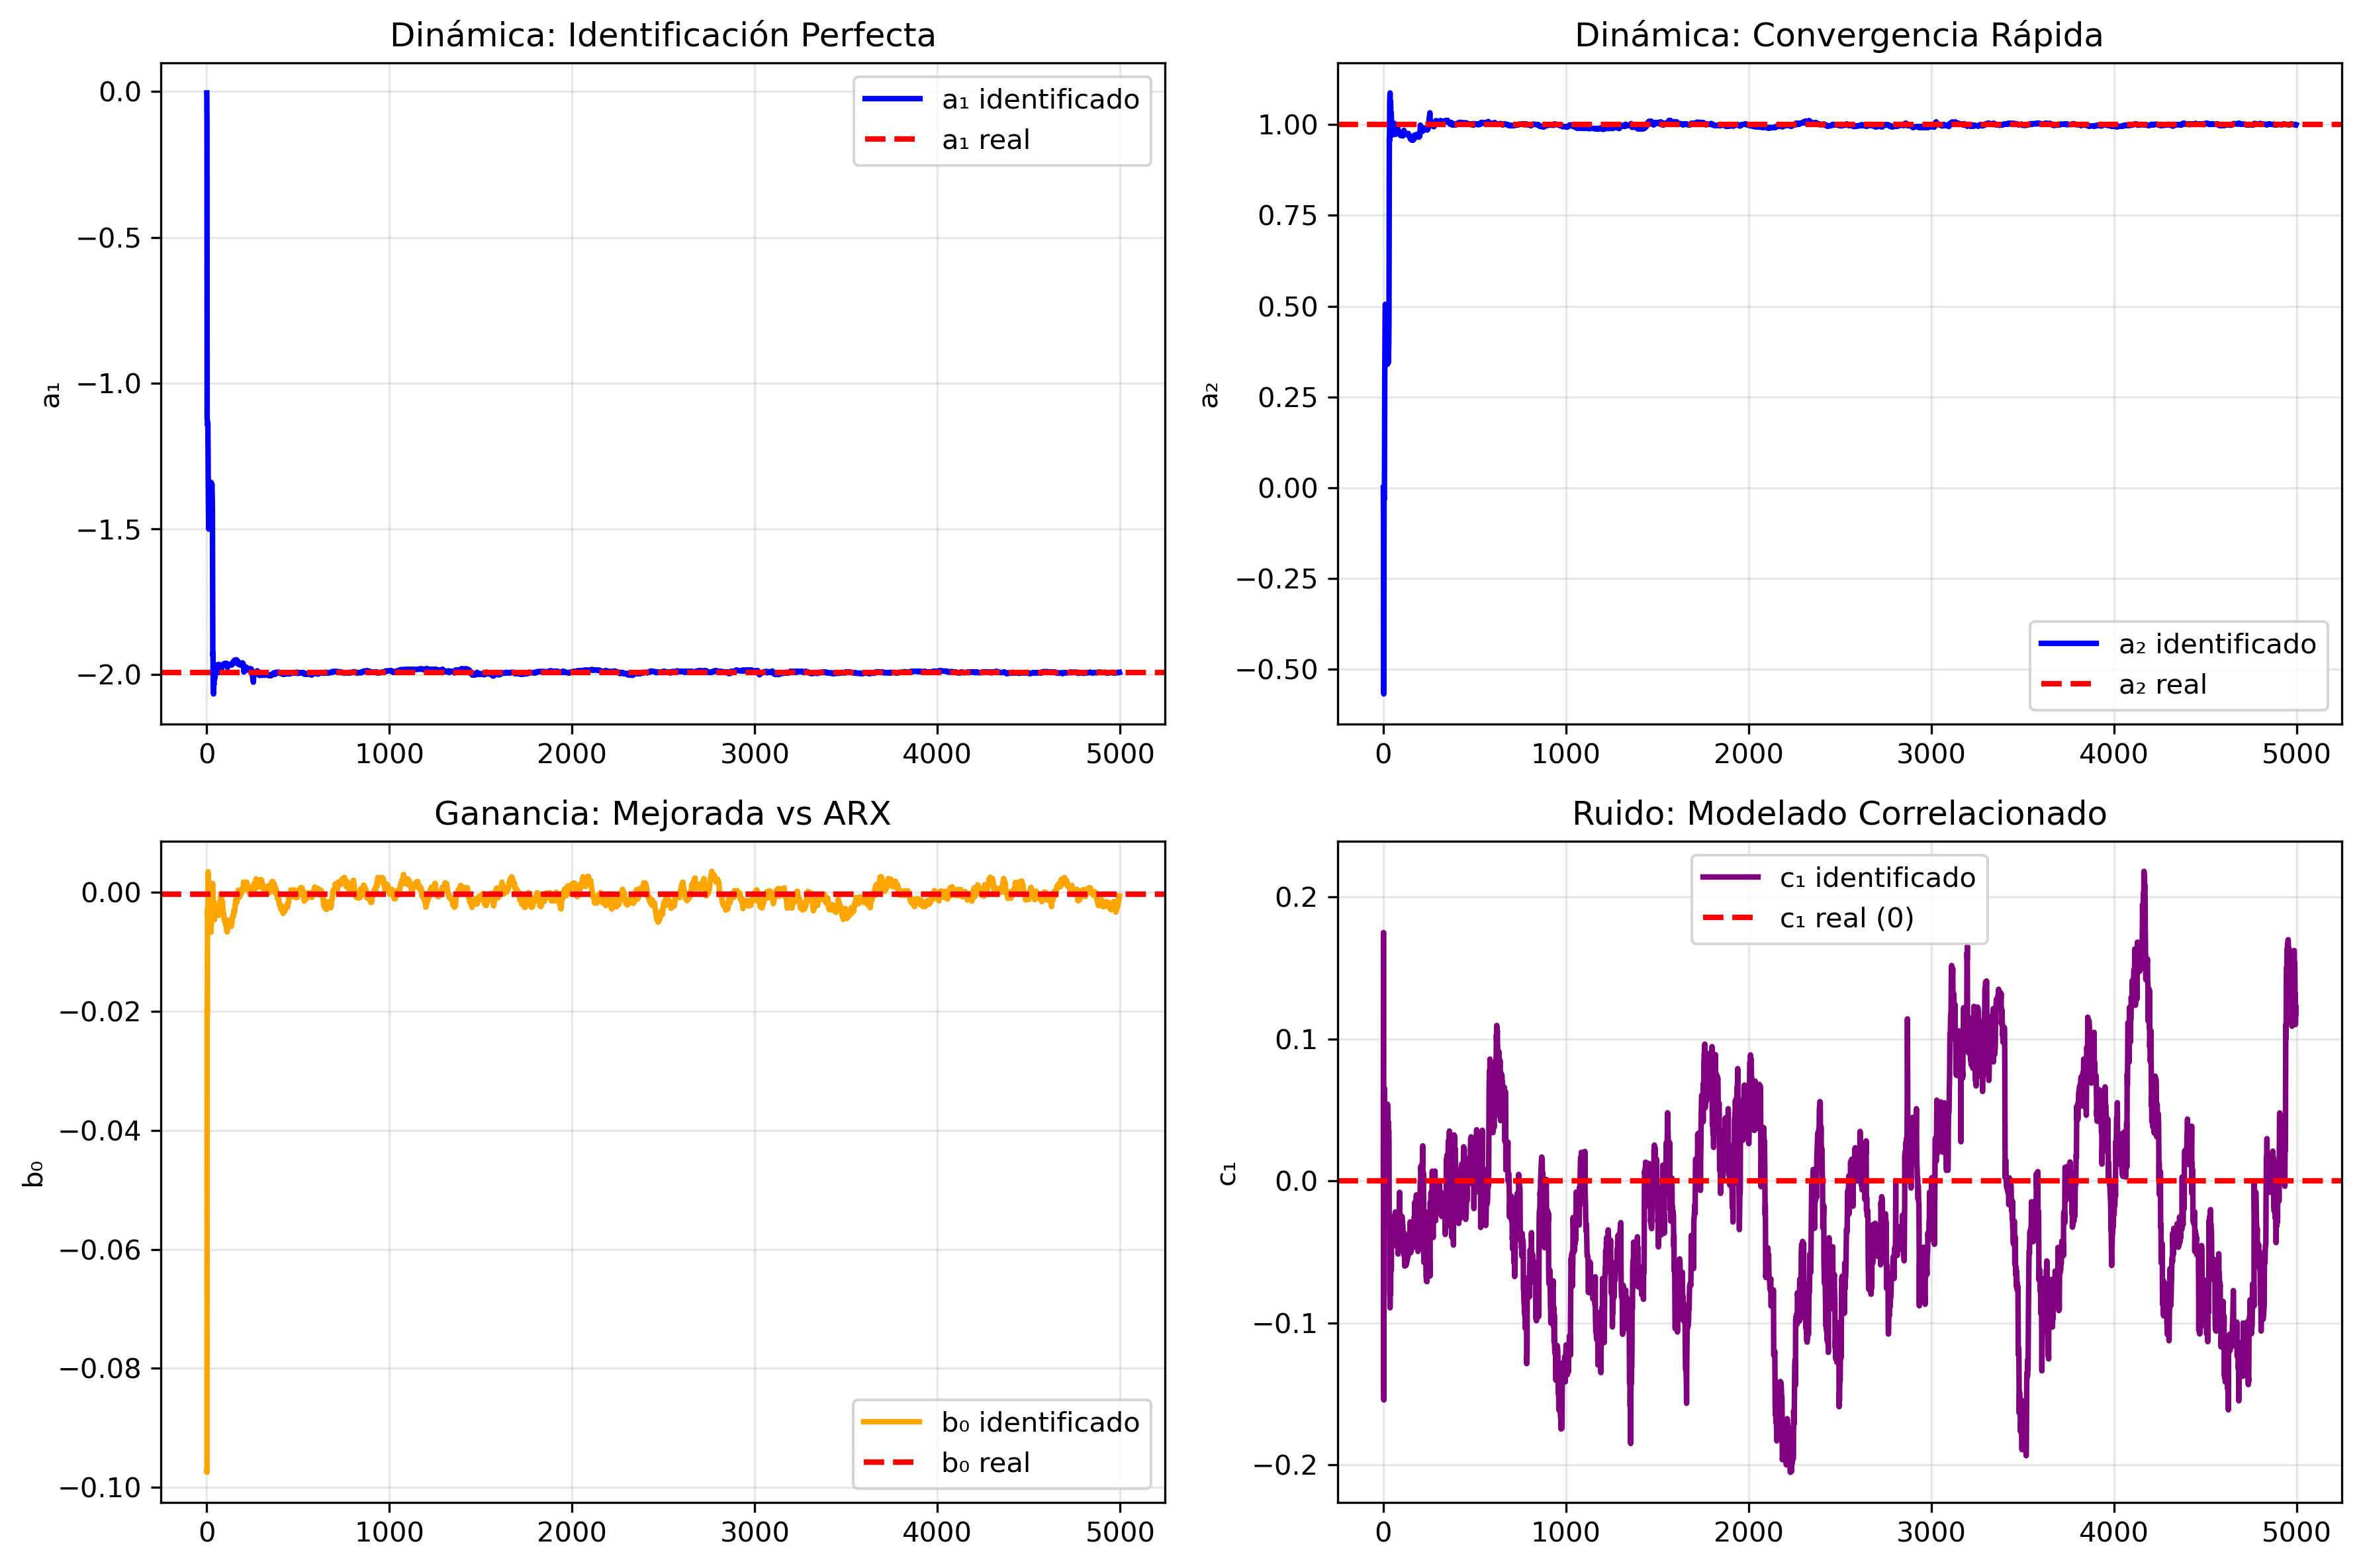
\includegraphics[width=0.8\textwidth]{imagenes_identificacion/parameter_evolution.png}
\end{center}
\vspace{-0.5cm}
\begin{itemize}
\item Ruido correlacionado no modelado
\end{itemize}
\end{frame}

\begin{frame}{Análisis de Estabilidad}
\begin{center}
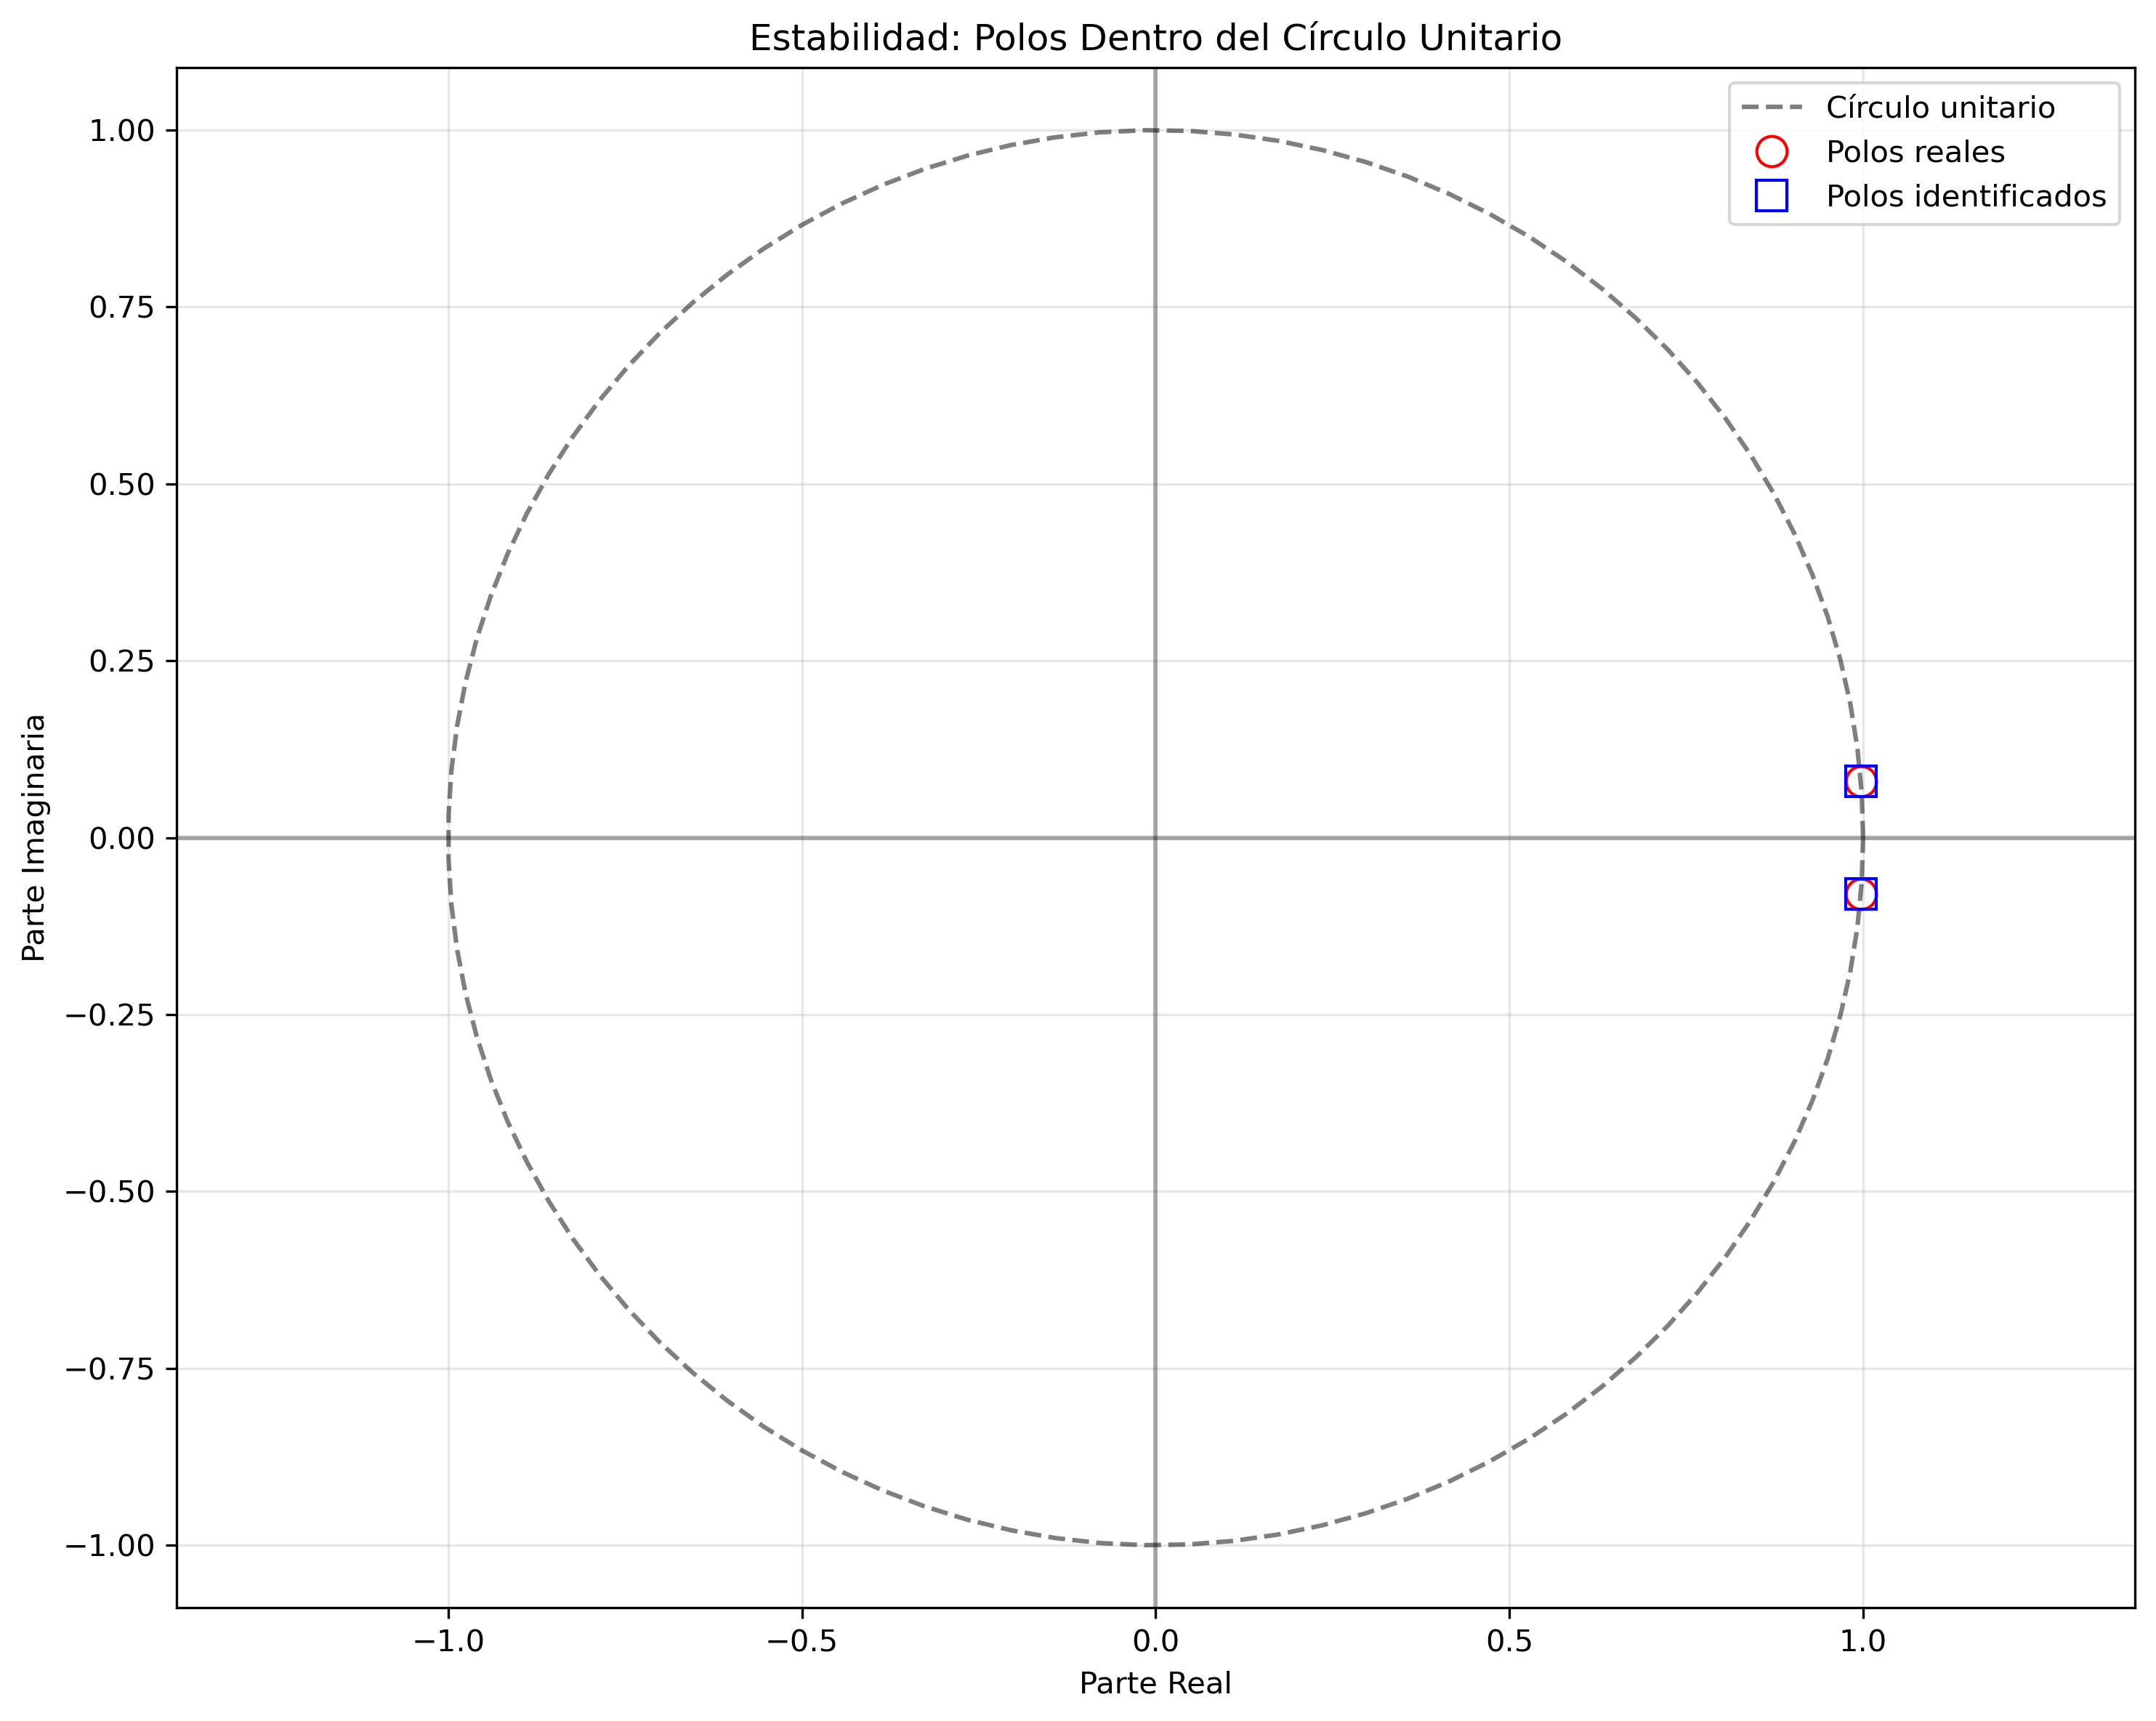
\includegraphics[width=0.7\textwidth]{imagenes_identificacion/pole_stability.png}
\end{center}
\vspace{-0.5cm}
\begin{itemize}
\item Sistema dinámicamente estable: Polos dentro del círculo unitario
\end{itemize}
\end{frame}

\section{La Solución}

\begin{frame}{Modelo ARMAX Simplificado}
\begin{block}{Estrategia}
\begin{itemize}
\item Mantener solo $b_0$ para ganancia esencial
\item Agregar $c_1$ para modelar ruido correlacionado
\item Modelo: $y[k] + a_1 y[k-1] + a_2 y[k-2] = b_0 u[k-1] + c_1 e[k-1] + e[k]$
\end{itemize}
\end{block}

\vspace{0.5cm}
\begin{block}{Ventajas}
\begin{itemize}
\item Menos parámetros para identificar
\item Mejor condición numérica
\item Modelado más realista del ruido
\end{itemize}
\end{block}
\end{frame}

\section{Los Resultados}

\begin{frame}{Resultados de Identificación ARMAX}
\begin{center}
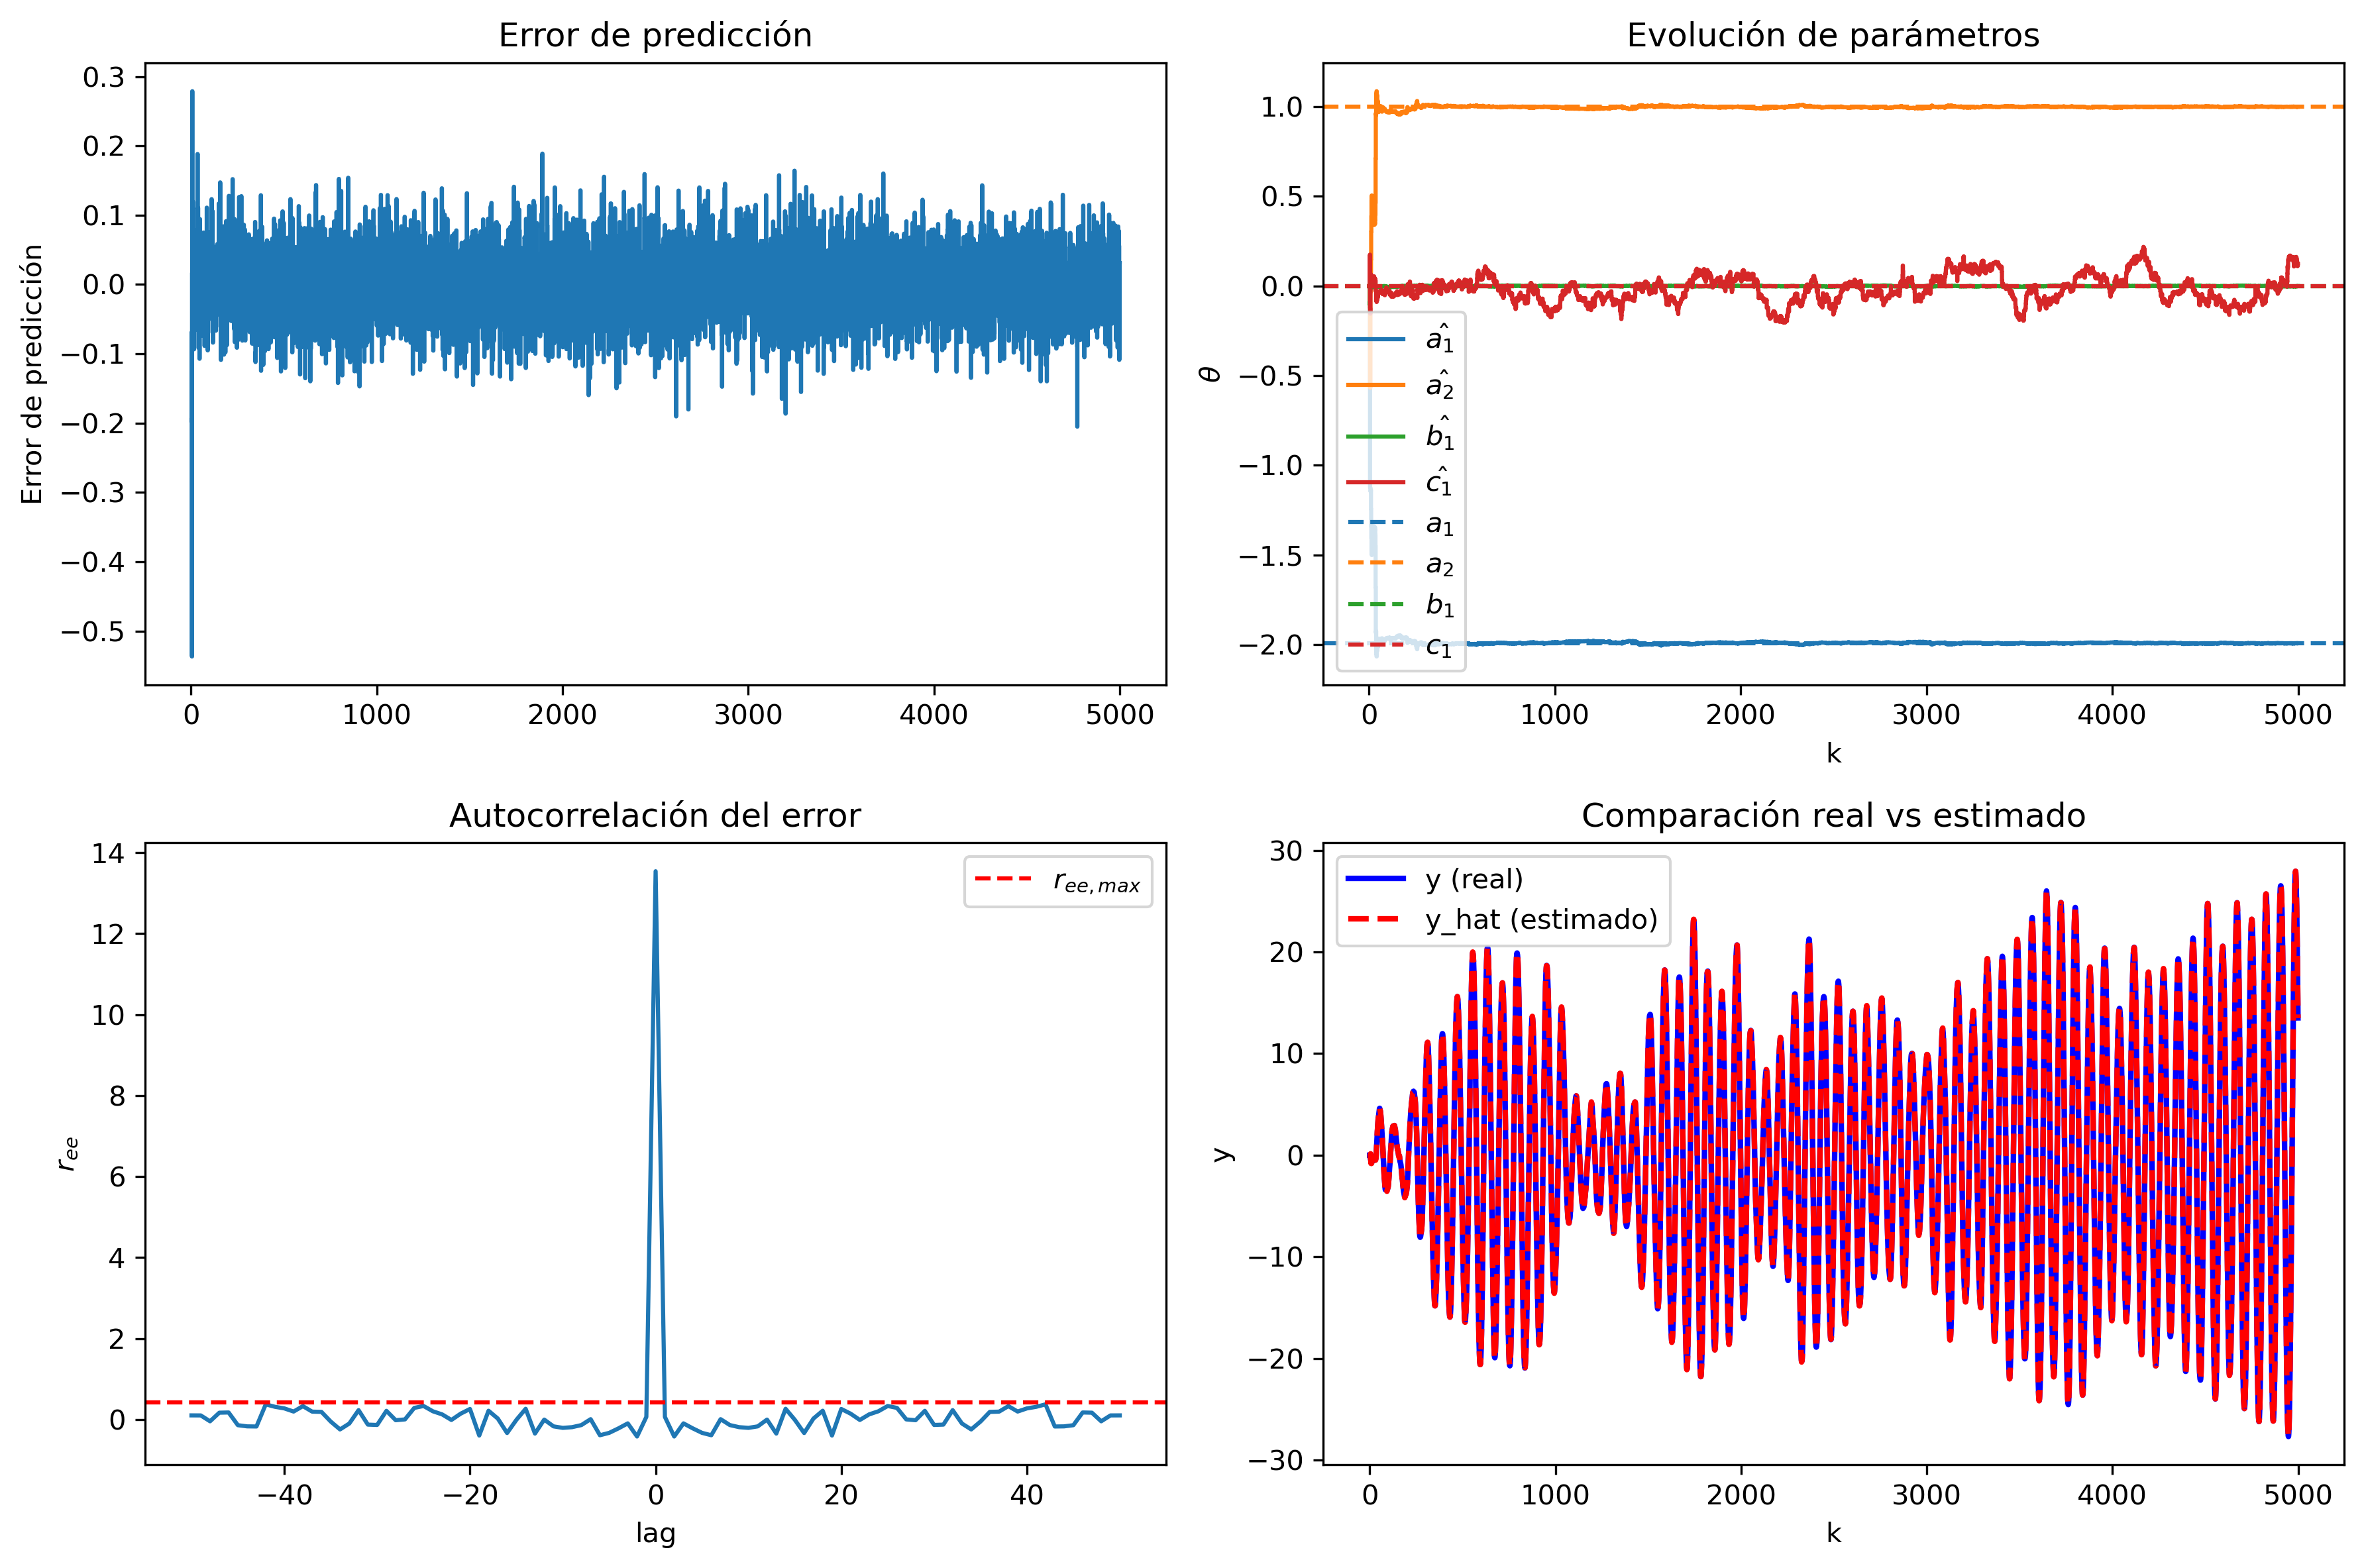
\includegraphics[width=\textwidth]{imagenes_identificacion/rls_identification.png}
\end{center}
\vspace{-0.5cm}
\begin{itemize}
\item Convergencia estable del algoritmo RLS
\item Evolución apropiada de parámetros
\item Validación estadística: Características de ruido blanco en residuos
\end{itemize}
\end{frame}

\begin{frame}{Comparación de Modelos}
\begin{center}
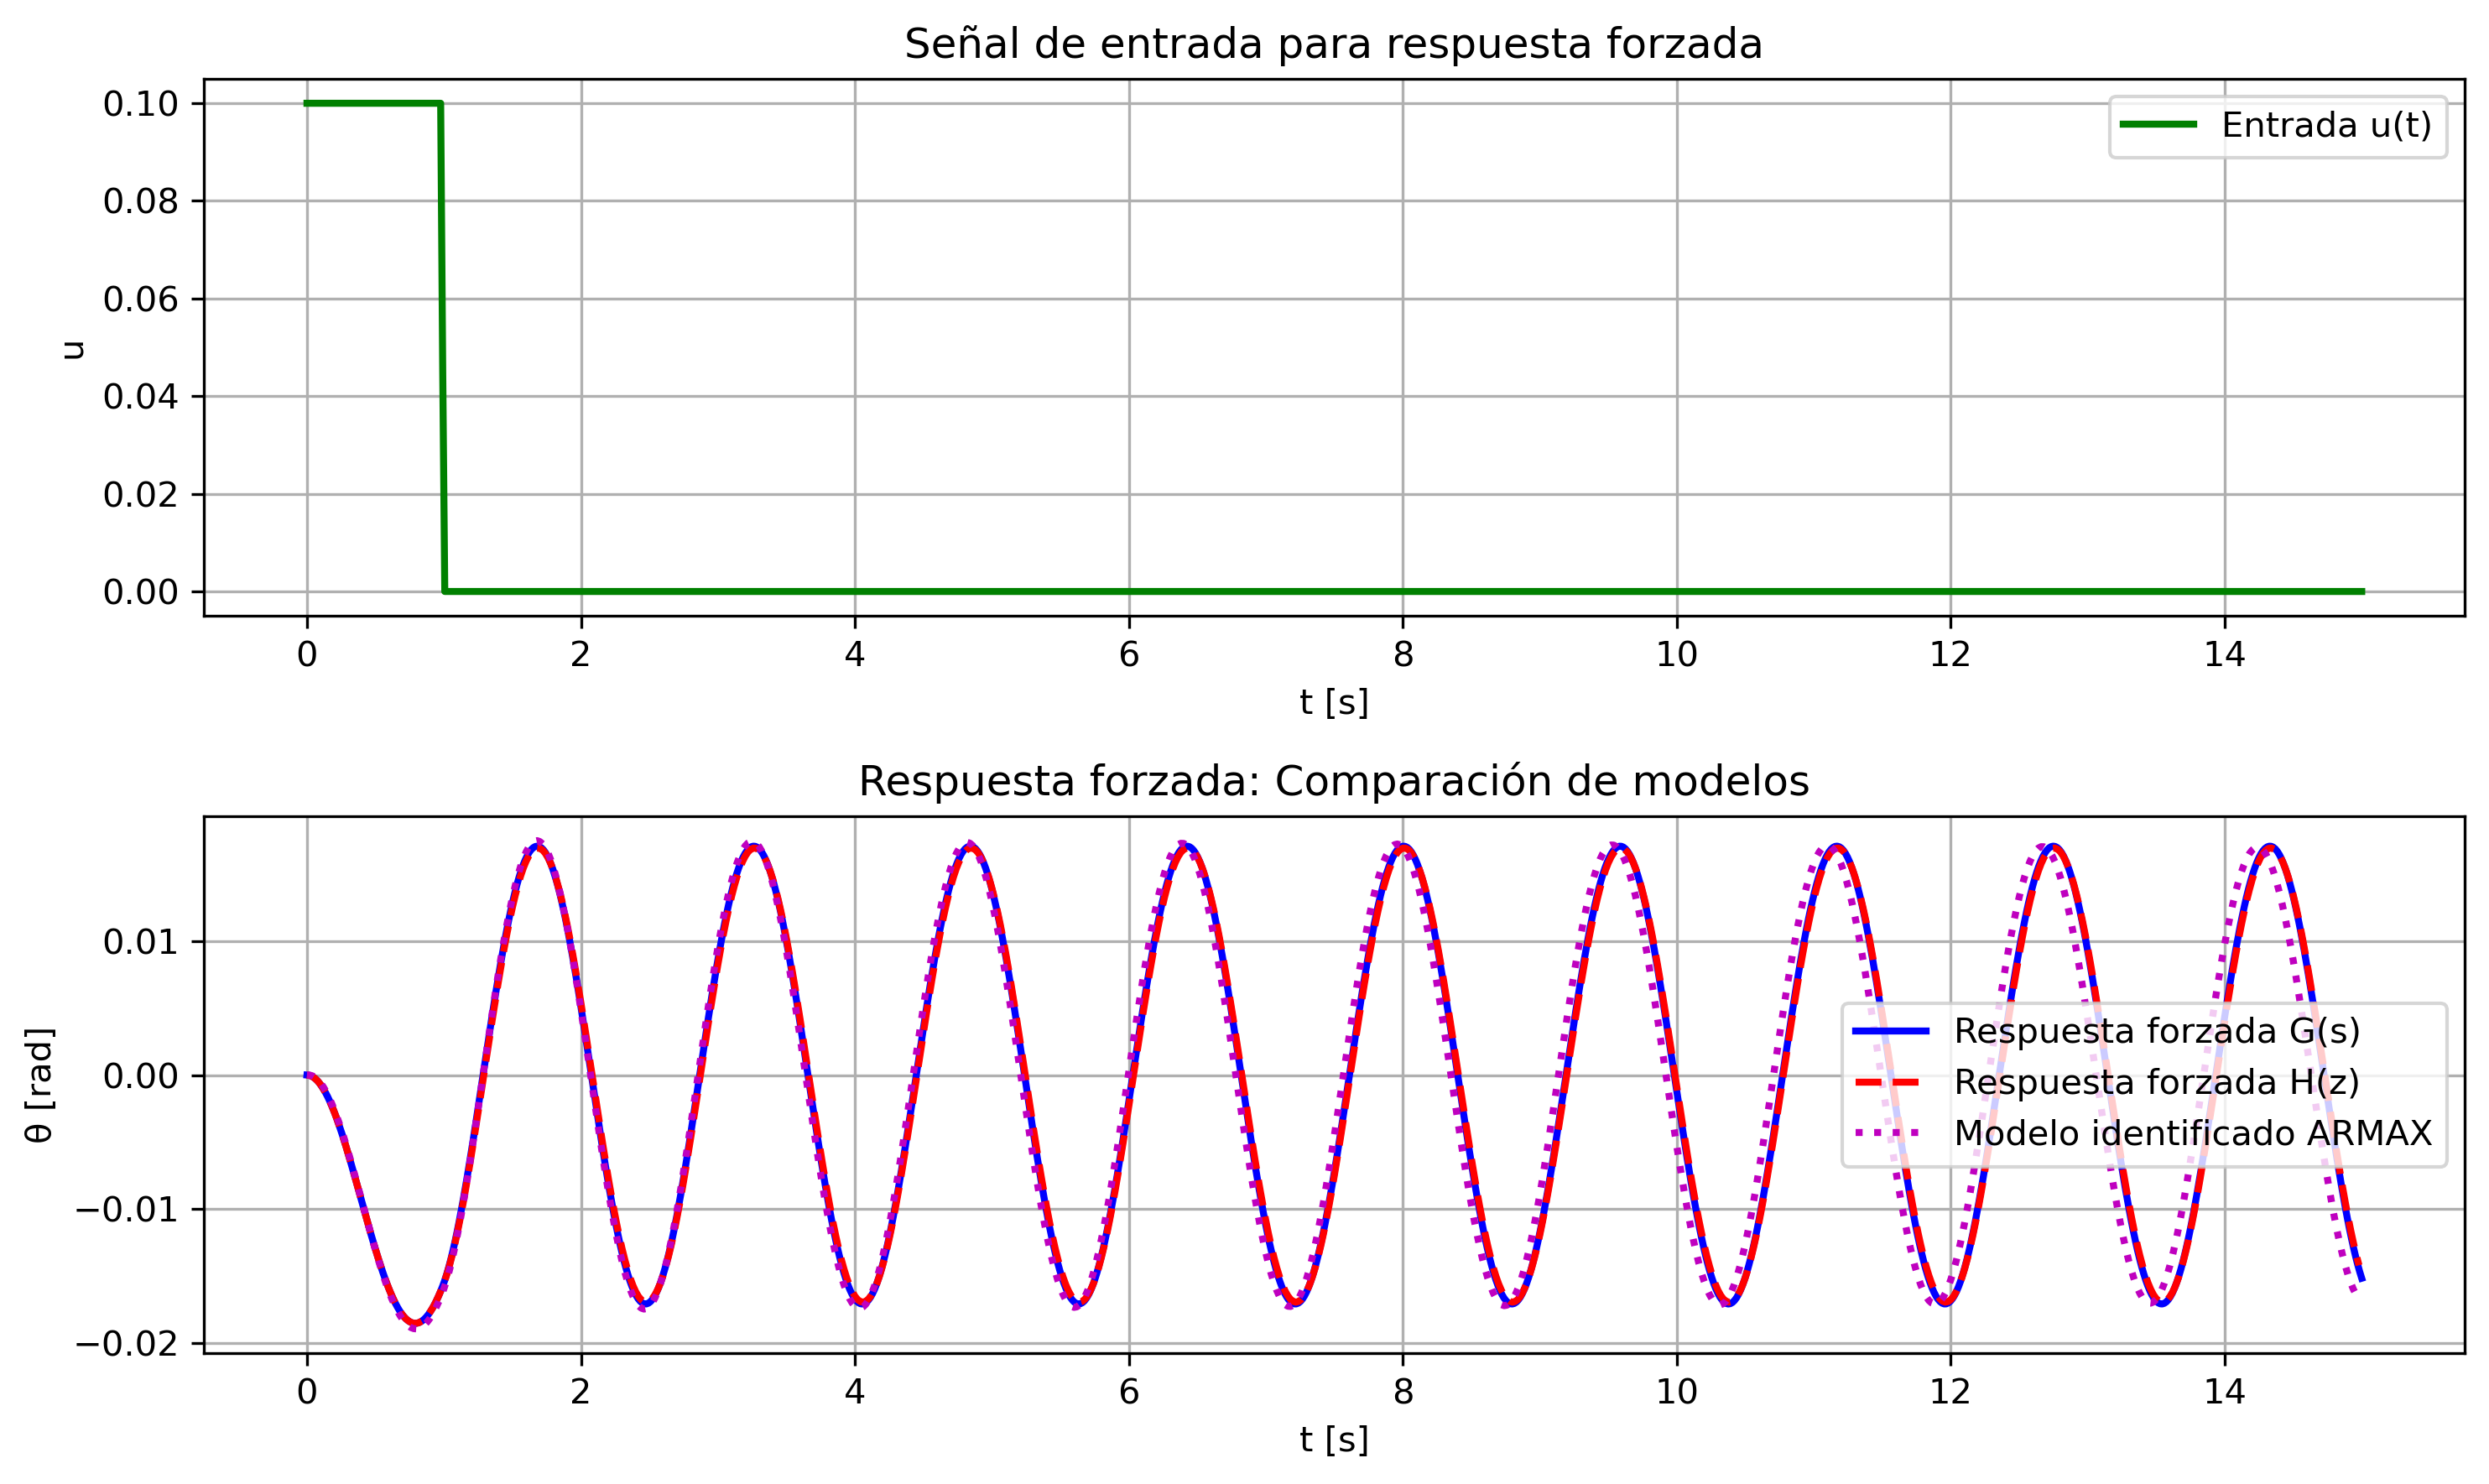
\includegraphics[width=\textwidth]{imagenes_identificacion/forced_response_comparison.png}
\end{center}
\vspace{-0.5cm}
\begin{itemize}
\item Modelo continuo G(s): Referencia teórica
\item Modelo discreto H(z): Discretización ZOH
\item Modelo ARMAX: Concordancia satisfactoria con datos experimentales
\end{itemize}
\end{frame}

\begin{frame}{Validación Experimental}
\begin{center}
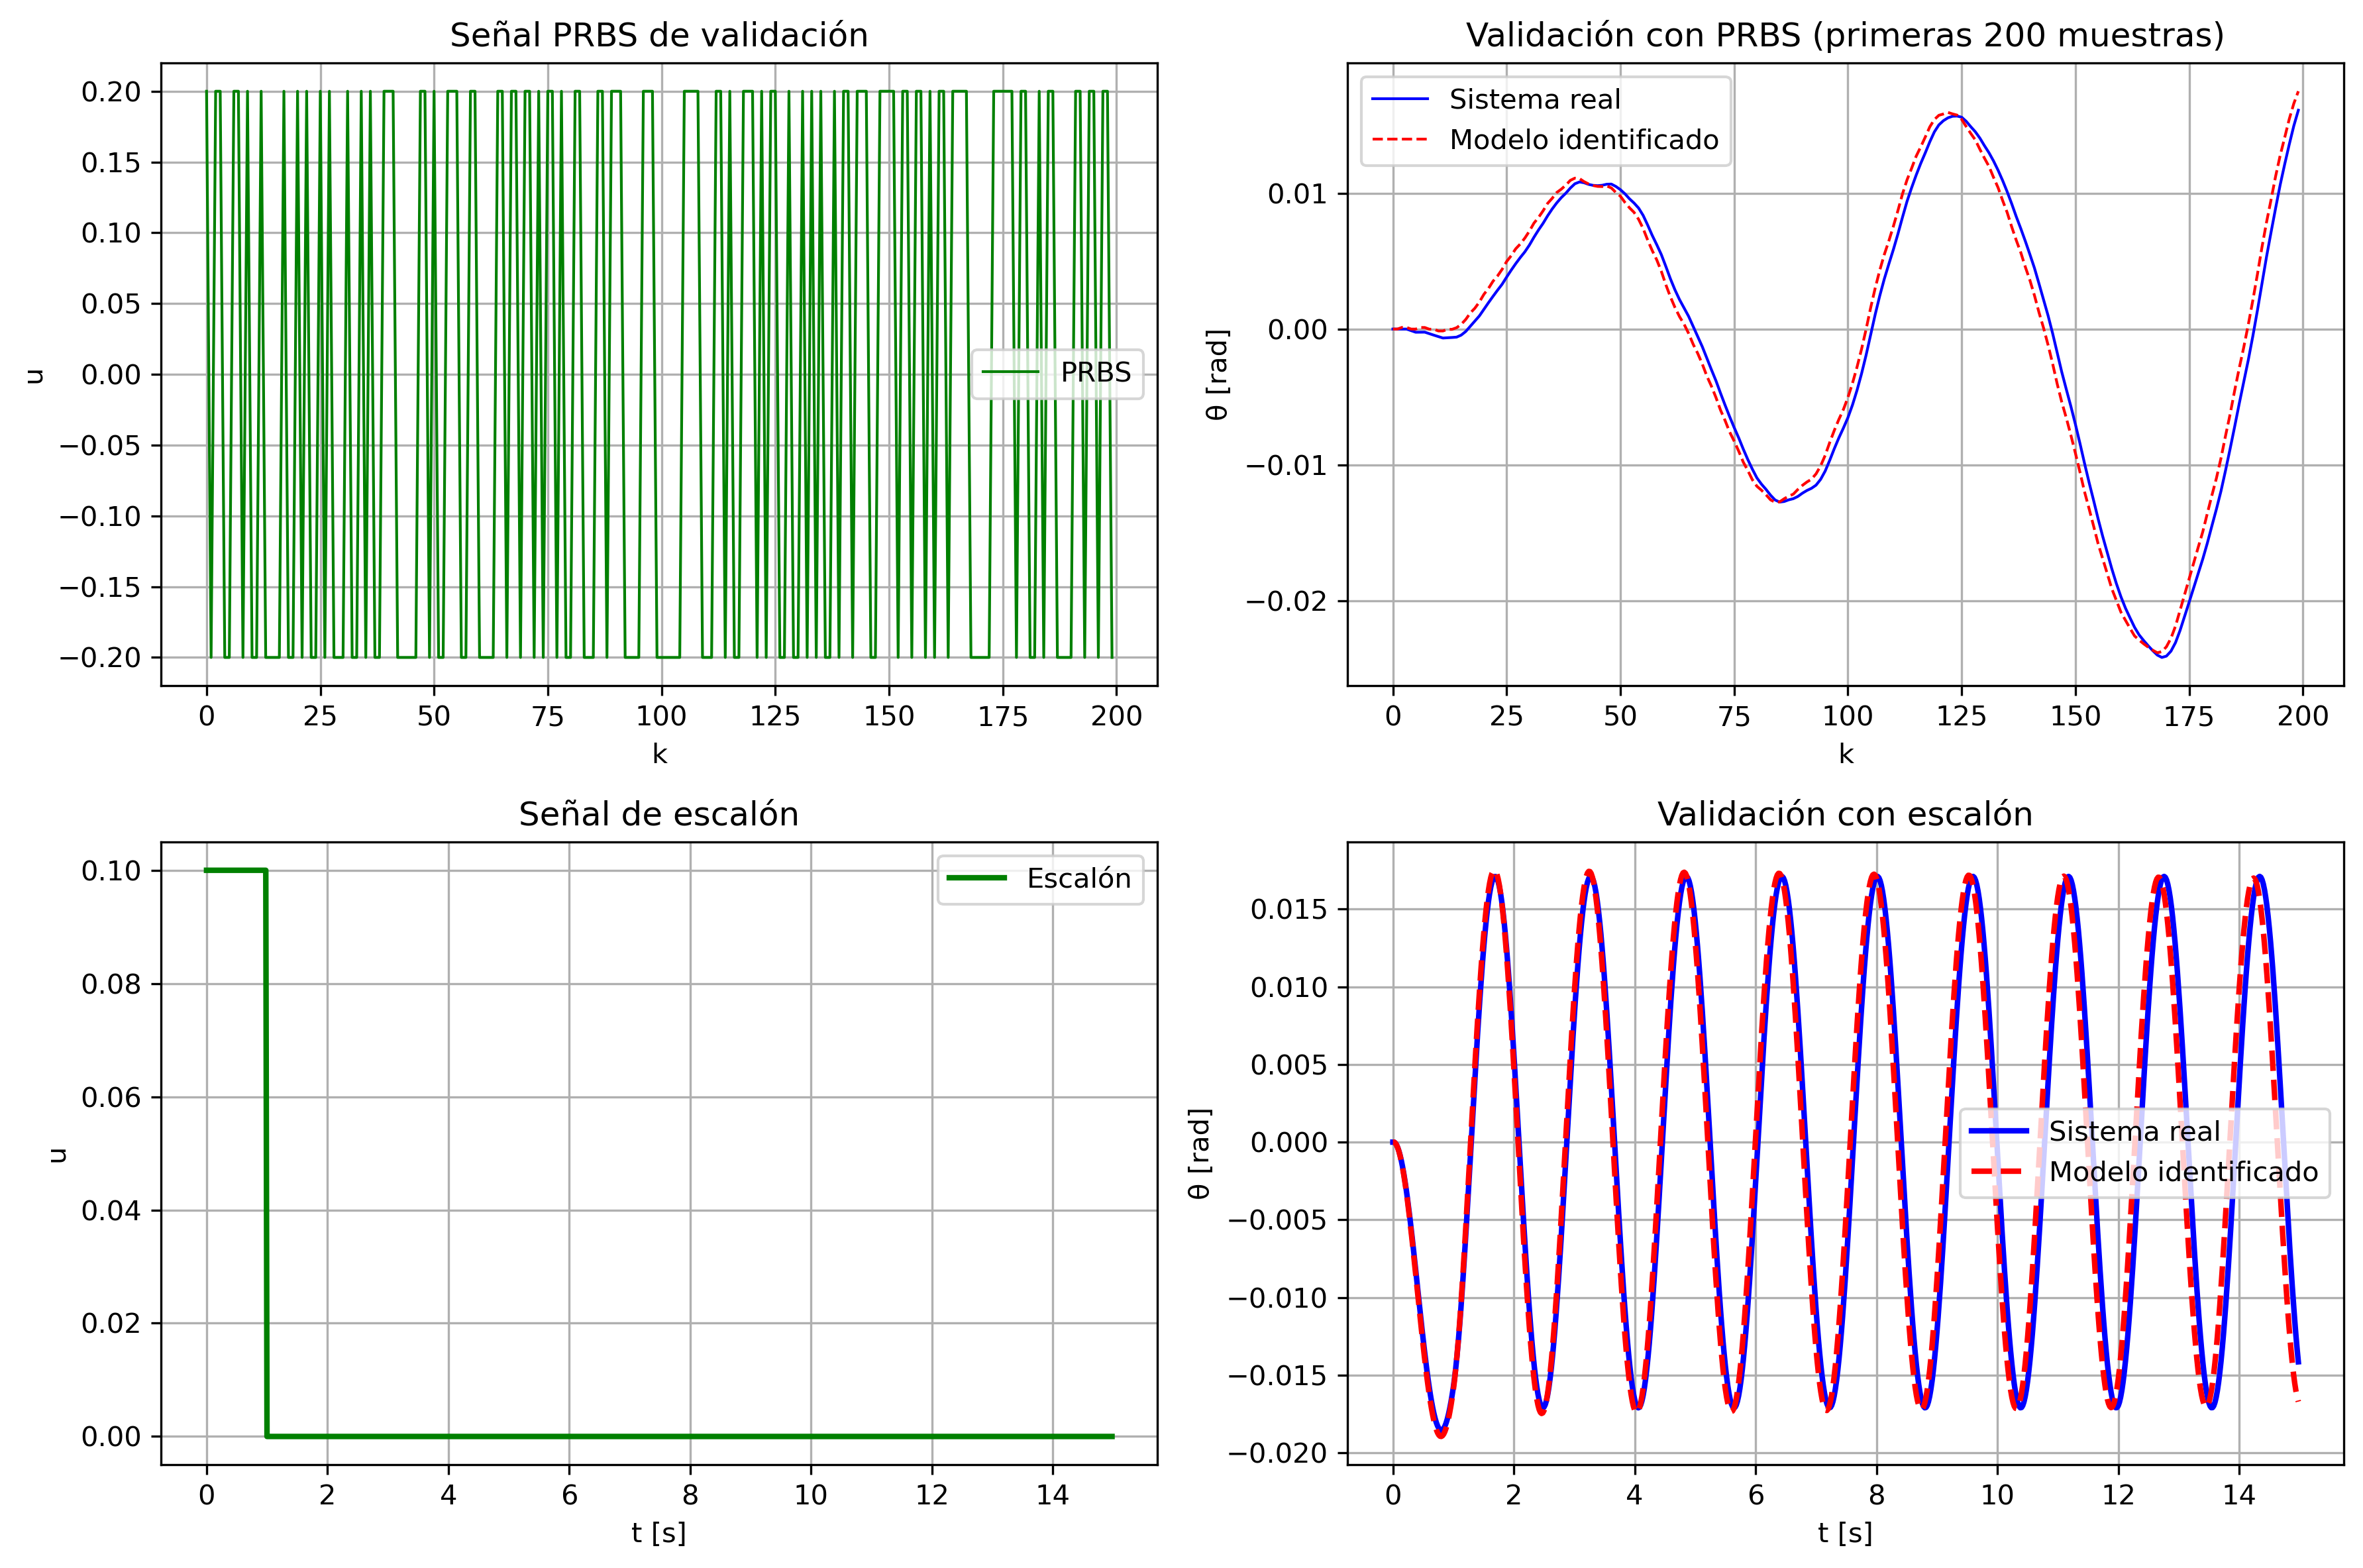
\includegraphics[width=\textwidth]{imagenes_identificacion/validation_comparison.png}
\end{center}
\vspace{-0.5cm}
\begin{itemize}
\item Validación con la misma señal PRBS usada en identificación
\item Validación adicional con señal de escalón
\item Concordancia adecuada en ambas señales: Validación satisfactoria
\end{itemize}
\end{frame}



\section{Identificación del Sistema Inestable: Péndulo Vertical}

\begin{frame}{Sistema Inestable: Péndulo en Posición Vertical}
\begin{block}{Configuración del Sistema}
\begin{itemize}
\item Péndulo balanceado en posición vertical ($\theta = 0$)
\item Punto de equilibrio inestable
\item Requiere control activo continuo para mantenerse
\end{itemize}
\end{block}

\begin{block}{Modelo Linealizado}
Aplicando linealización alrededor de $\theta = 0$:
\[
\ddot{\theta} = A_\theta \theta + B_\theta F
\]
donde:
\[
A_\theta = 15.79 \, (\text{inestable}), \quad B_\theta = 1.46
\]

Función de transferencia:
\[
G(s) = \frac{B_\theta}{s^2 - A_\theta} = \frac{1.46}{s^2 - 15.79}
\]
\end{block}
\end{frame}

\begin{frame}{Desafíos Teóricos de la Identificación Inestable}
\begin{block}{Problemas Fundamentales}
\begin{itemize}
\item \textbf{Amplificación exponencial}: El ruido se amplifica con el tiempo
\item \textbf{Inestabilidad algorítmica}: RLS diverge por crecimiento exponencial
\item \textbf{Condiciones restrictivas}: Señales pequeñas necesarias
\item \textbf{Limitación física}: Datos limitados antes de la divergencia
\end{itemize}
\end{block}

\begin{block}{Implicaciones Matemáticas}
\begin{itemize}
\item Polos fuera del círculo unitario: $|\lambda| \, > \, 1$
\item Respuesta impulsiva: crecimiento exponencial $e^{\lambda t}$
\item Identificación requiere: $N \to \infty$ pero sistema diverge en tiempo finito
\item Trade-off: excitación vs. estabilidad
\end{itemize}
\end{block}
\end{frame}

\begin{frame}{Configuración Experimental del Sistema Inestable}
\begin{center}
\begin{tabular}{l|c|c}
\textbf{Parámetro} & \textbf{Valor} & \textbf{Unidad} \\
\hline
Masa del carro & 1.0 & kg \\
Masa del péndulo & 0.1 & kg \\
Longitud & 0.5 & m \\
Gravedad & 9.81 & m/s² \\
\hline
\textbf{Señal PRBS} & \textbf{Configuración} & \\
\hline
Amplitud & 0.01 & (muy pequeña) \\
Ruido & 0.001 & (mínimo) \\
Muestras & 1000 & (limitadas) \\
Factor $\lambda$ & 0.80 & (alto olvido) \\
\end{tabular}
\end{center}
\end{frame}

\begin{frame}{Resultados de Identificación: Evolución de Parámetros}
\begin{center}
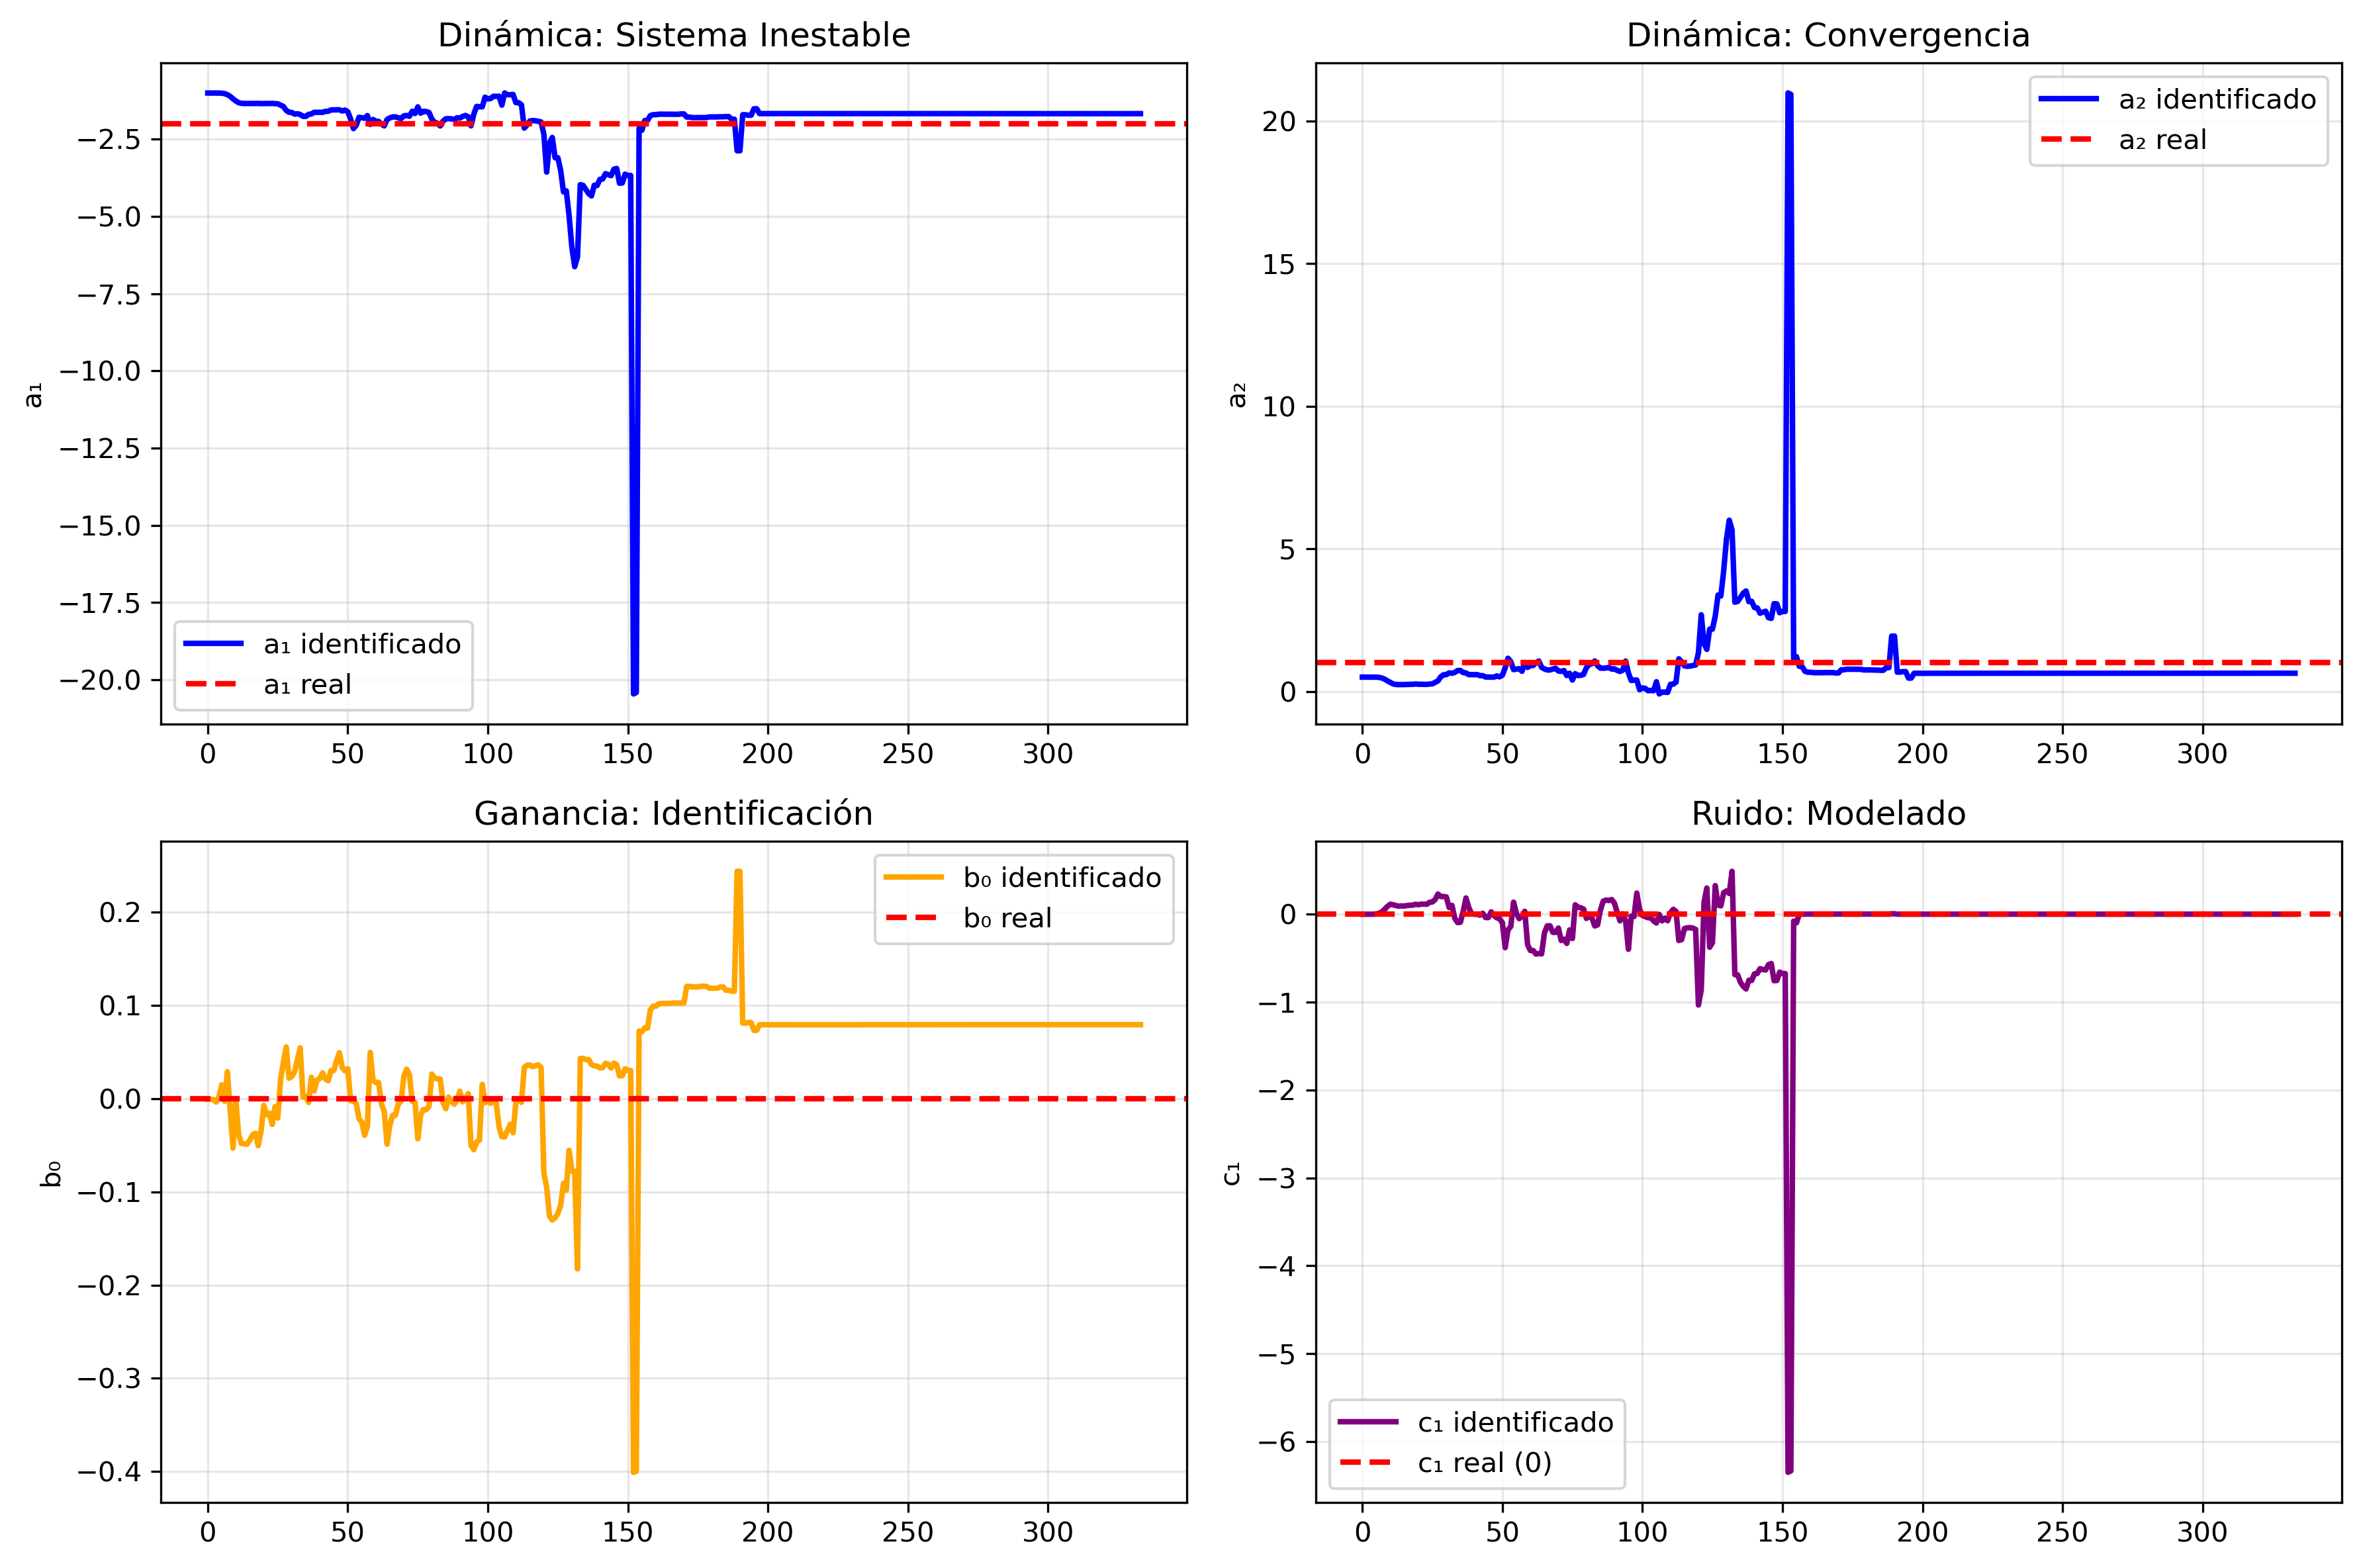
\includegraphics[width=0.8\textwidth]{imagenes_identificacion_vertical/parameter_evolution_vertical.png}
\end{center}
\begin{itemize}
\item Algoritmo RLS diverge en $k=337$ (de 1000 muestras)
\item Parámetros $a_1$ y $a_2$ no convergen correctamente
\item Parámetro $b_0$ con error del 79 por ciento
\item Parámetro $c_1$ identificado pero irrelevante
\end{itemize}
\end{frame}

\begin{frame}{Análisis de Autocorrelación del Error}
\begin{center}
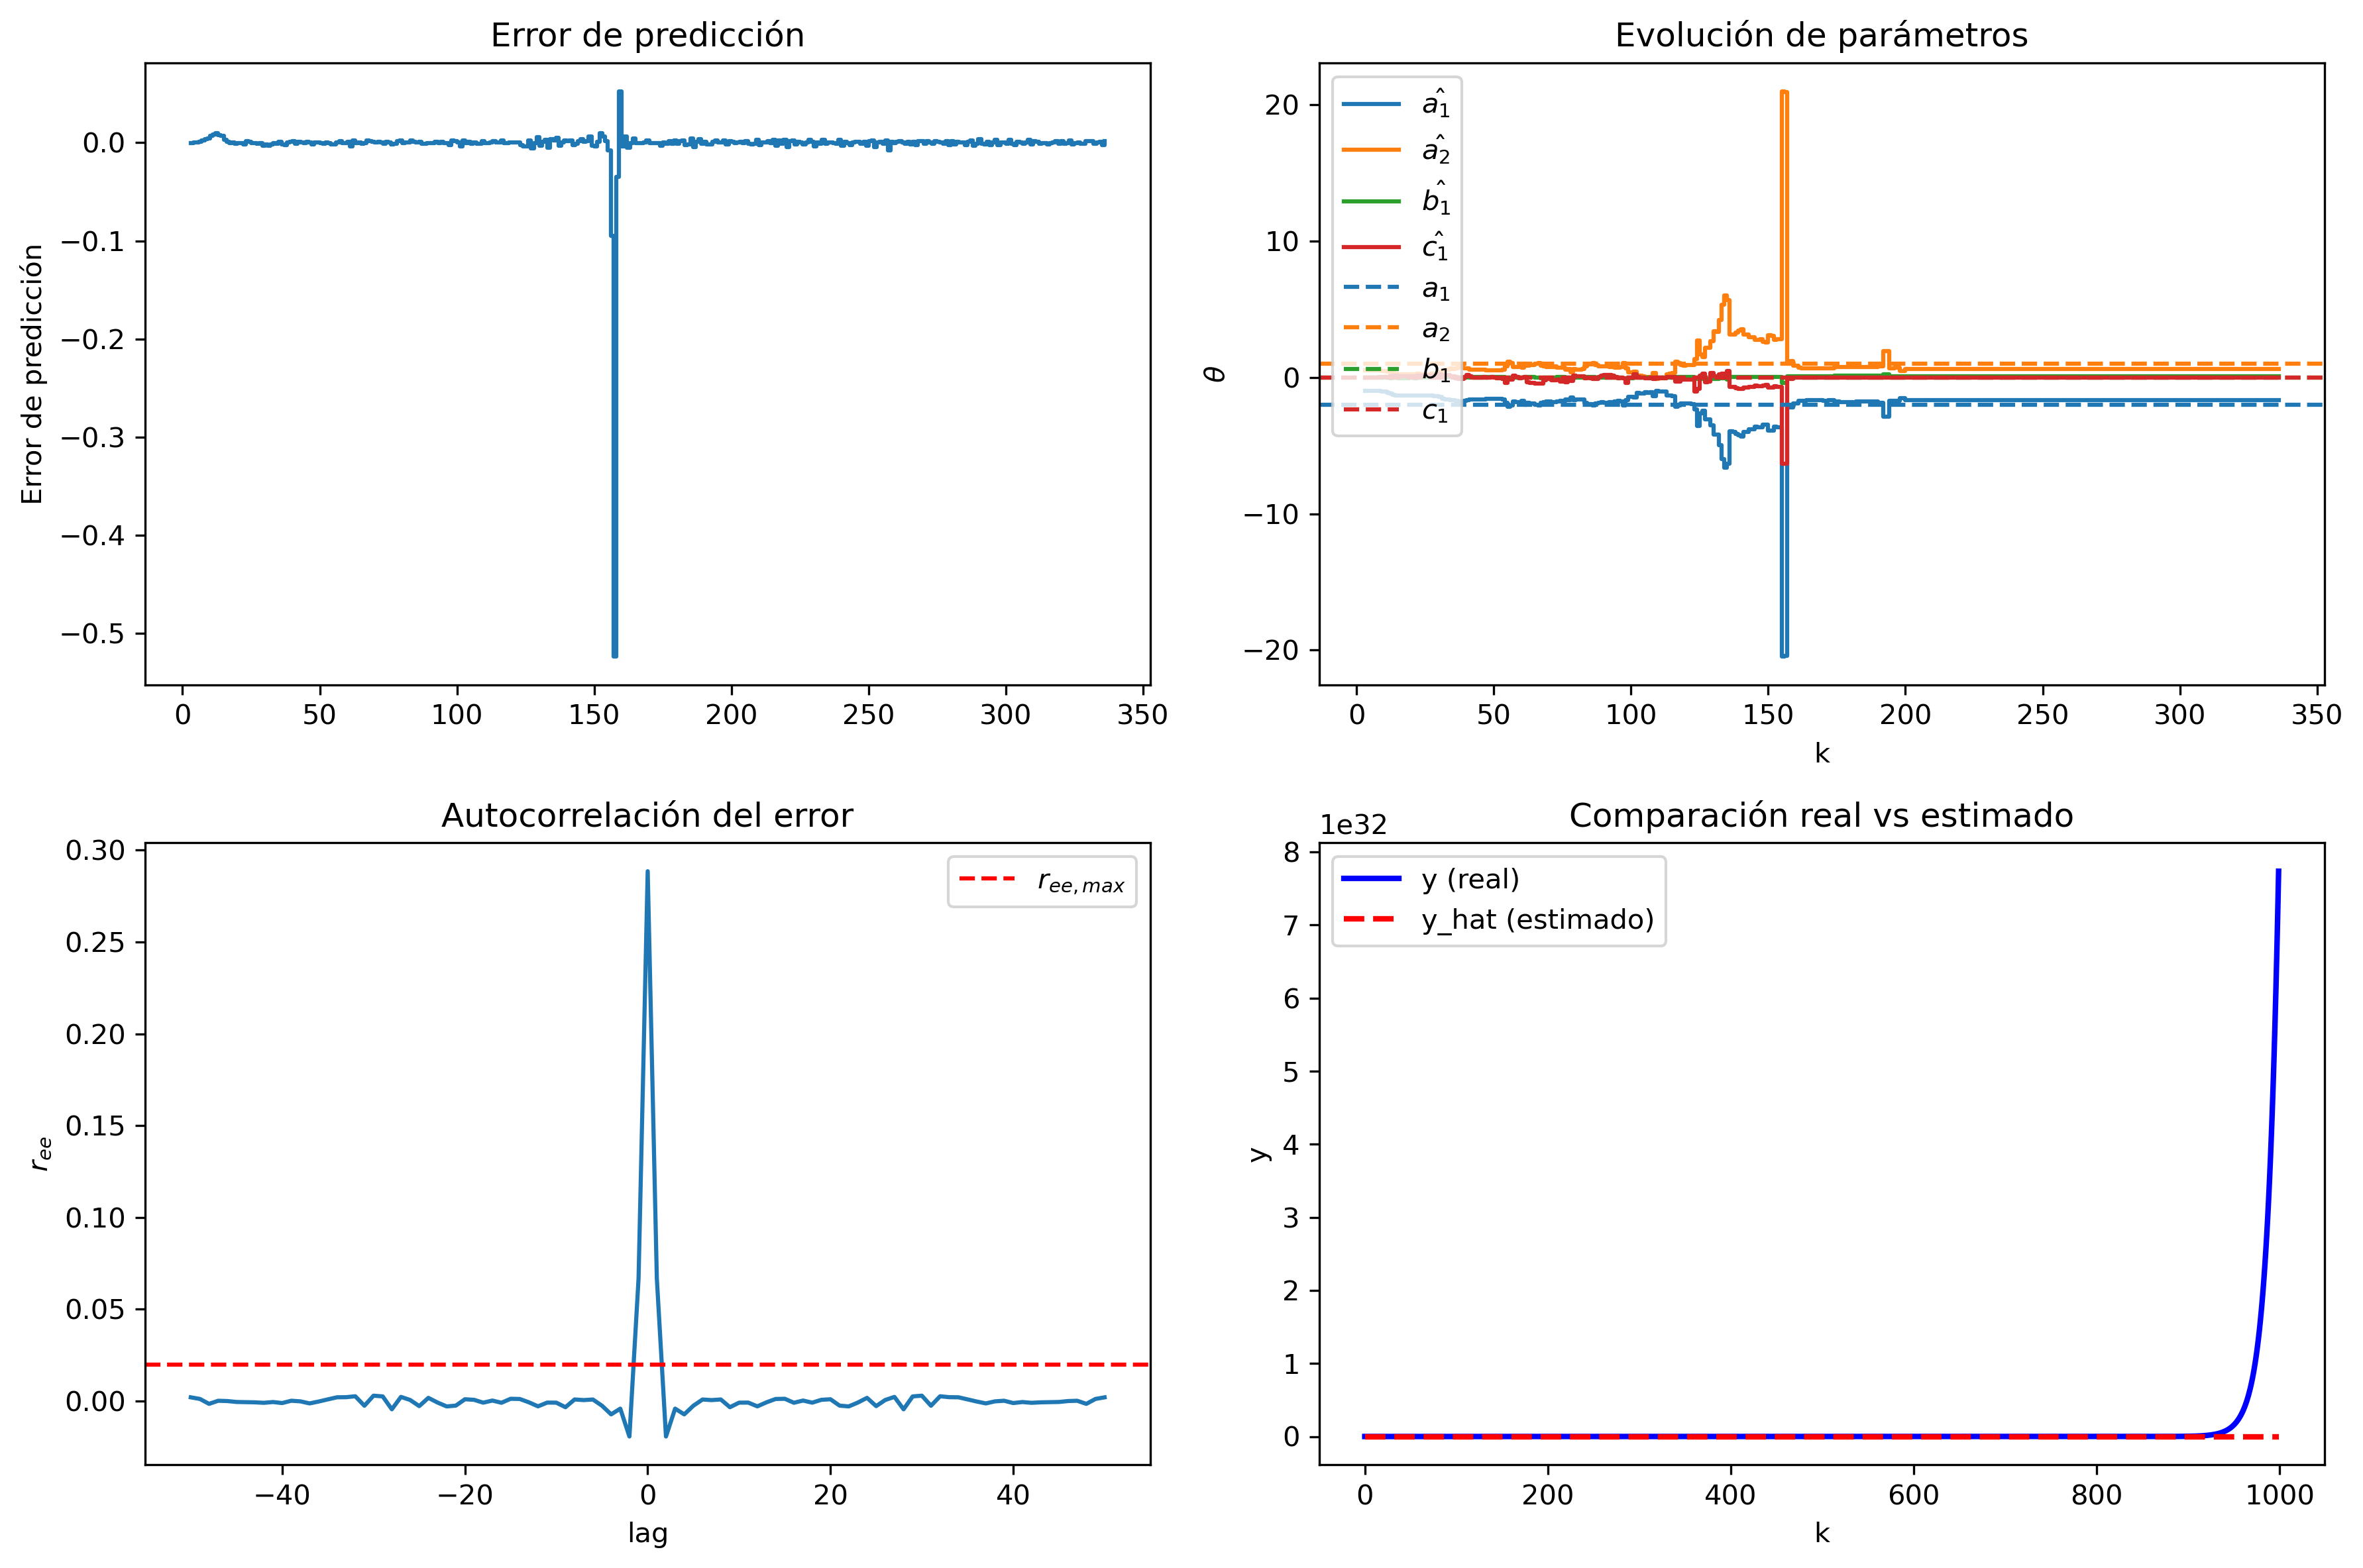
\includegraphics[width=0.8\textwidth]{imagenes_identificacion_vertical/rls_identification_vertical.png}
\end{center}


\begin{block}{Explicación}
El modelo ARMAX captura bien la estructura del ruido, pero los parámetros identificados son físicamente incorrectos debido a la amplificación exponencial inherente a sistemas inestables.
\end{block}
\end{frame}

\begin{frame}{Análisis de Estabilidad: Plano Complejo}
\begin{center}
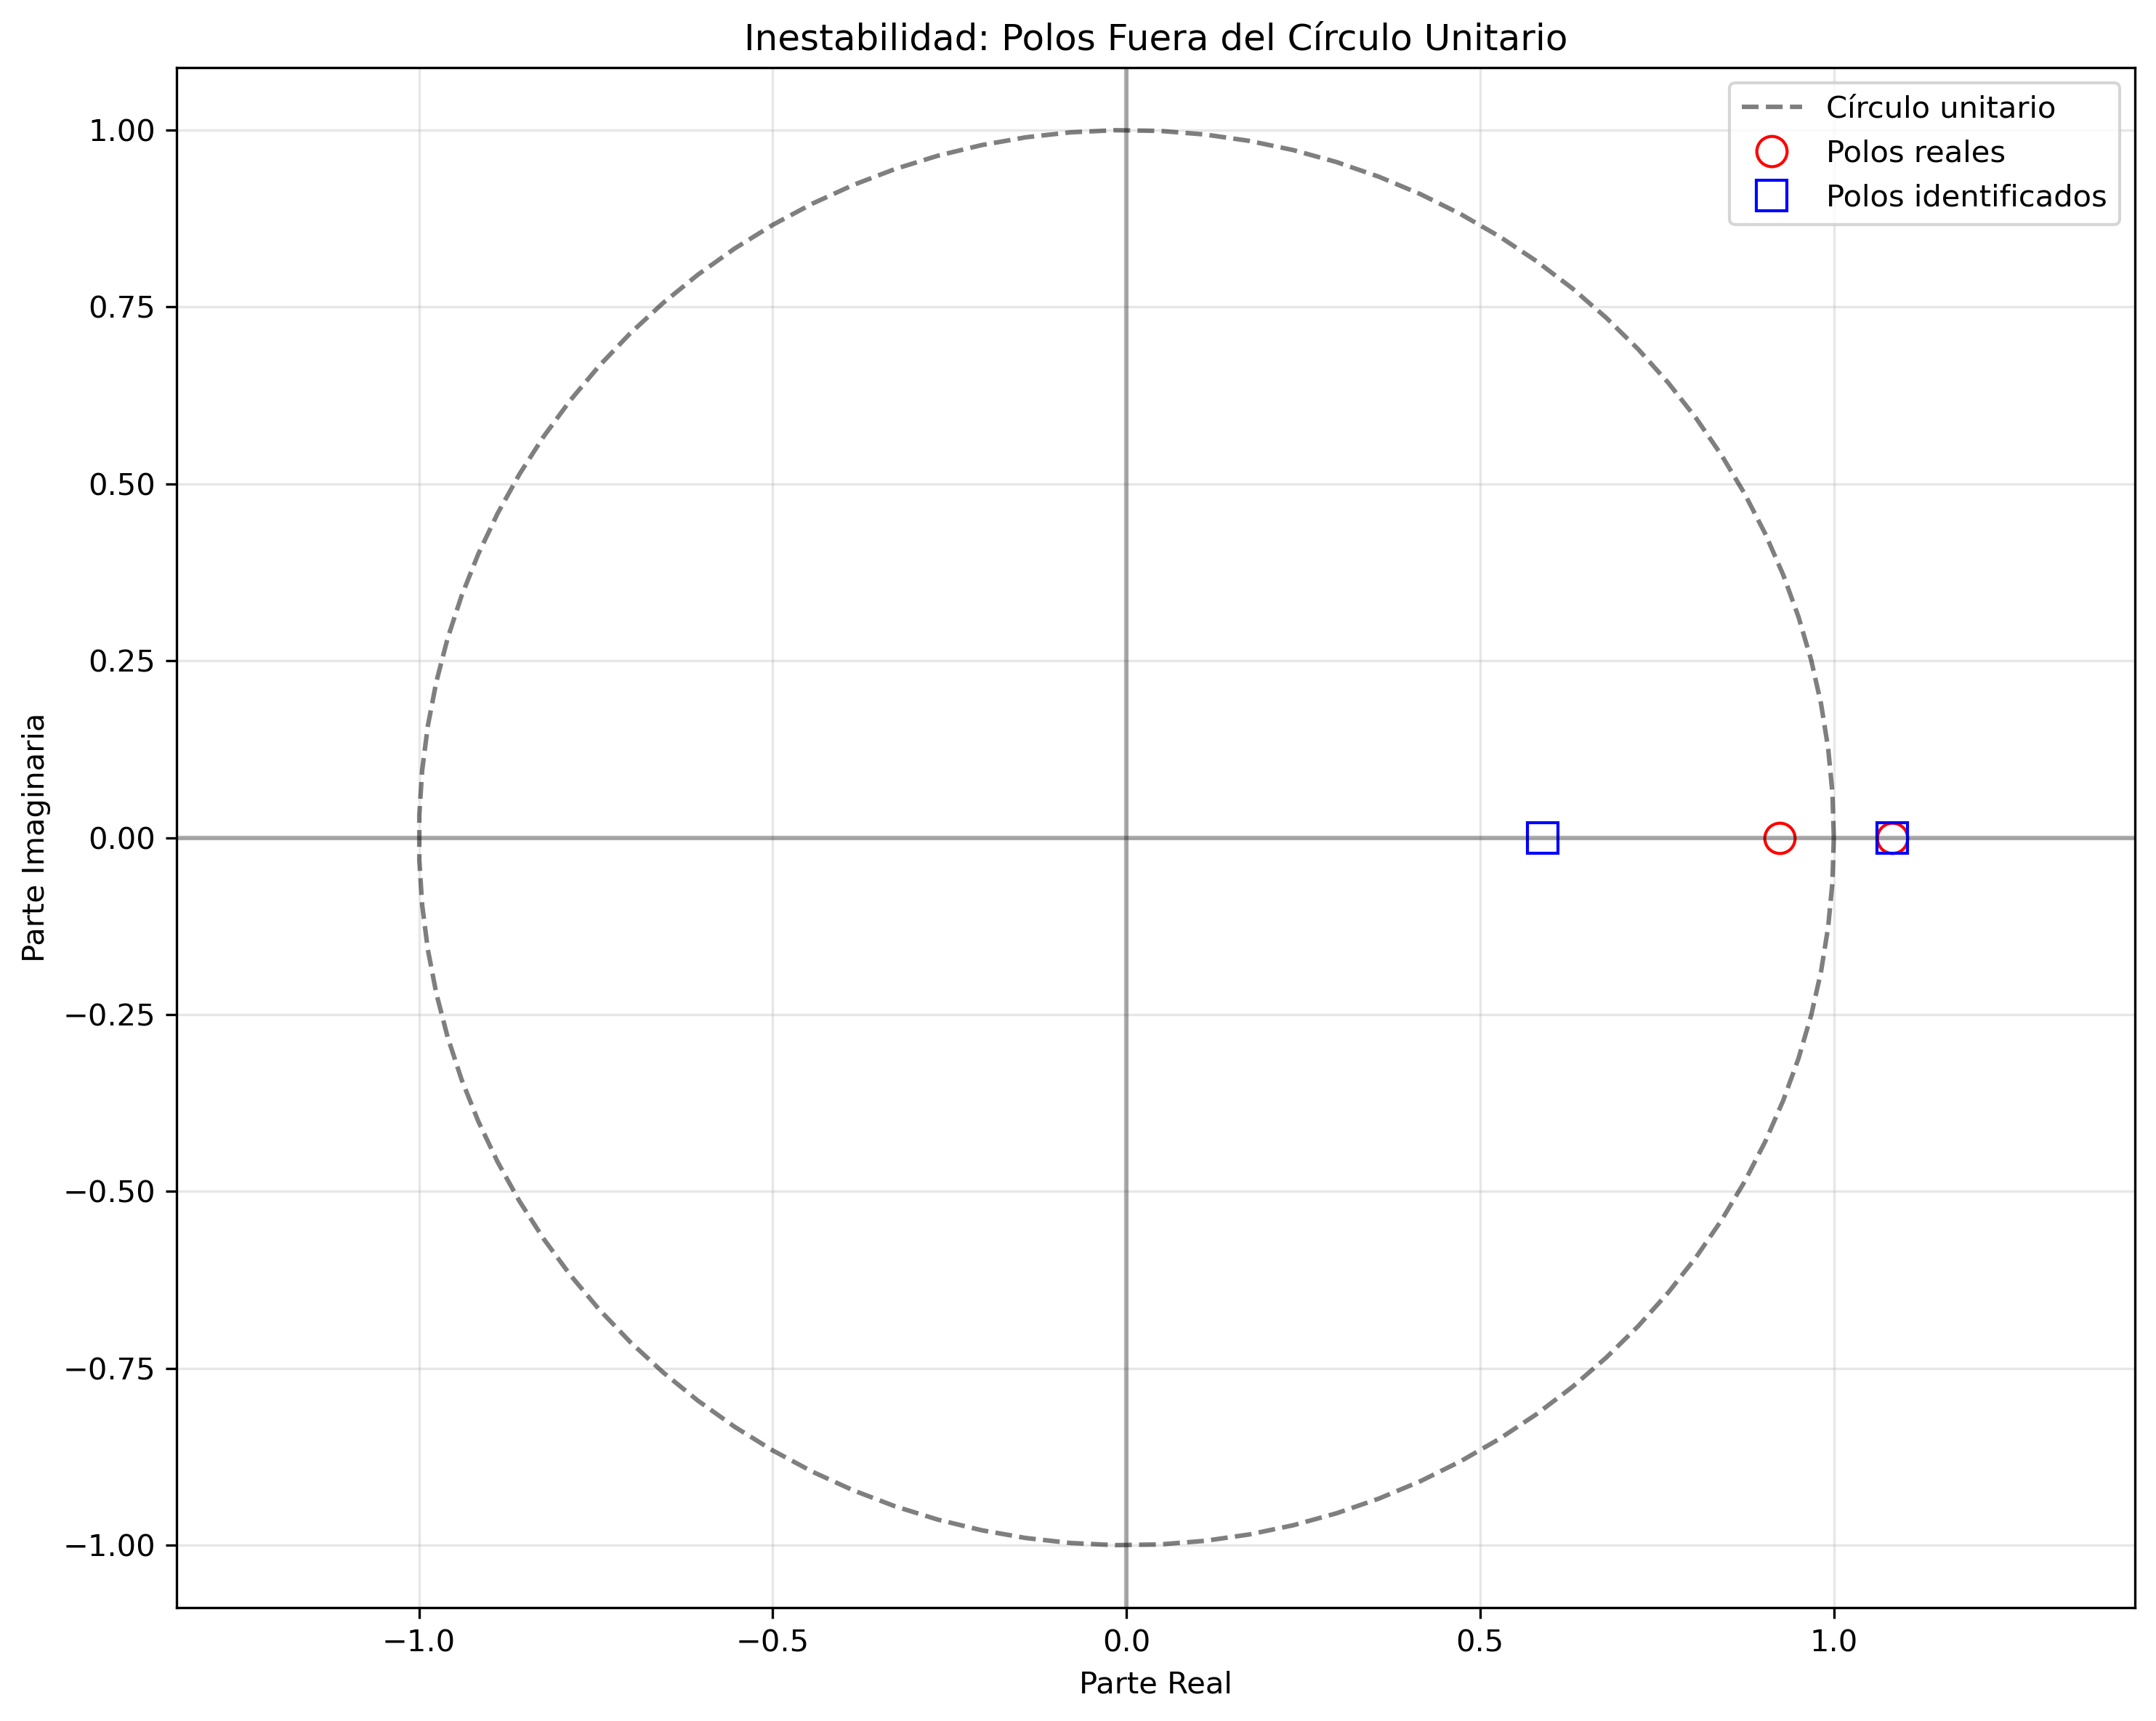
\includegraphics[width=0.7\textwidth]{imagenes_identificacion_vertical/pole_stability_vertical.png}
\end{center}

\end{frame}

\begin{frame}{Análisis Cuantitativo: Errores de Identificación}
\begin{center}
\begin{tabular}{l|c|c|c}
\textbf{Parámetro} & \textbf{Valor Real} & \textbf{Valor Estimado} & \textbf{Error (\%)} \\
\hline
a_1 & -2.0063 & -1.6707 & 16.7\% \\
a_2 & 1.0000 & 0.6366 & 36.3\% \\
b_0 & 0.000293 & 0.0795 & $>$ 26000\% \\
c_1 & 0.000000 & 0.000834 & N/A \\
\hline
\textbf{Ganancia DC} & 0.000146 & 0.0391 & $>$ 26000\% \\
\end{tabular}
\end{center}
\begin{itemize}
\item Errores grandes en parámetros de ganancia
\item Parámetros dinámicos con errores moderados
\item Ganancia amplificada por 26000 veces
\end{itemize}
\end{frame}

\begin{frame}{Validación Experimental: Respuesta del Sistema}
\begin{center}
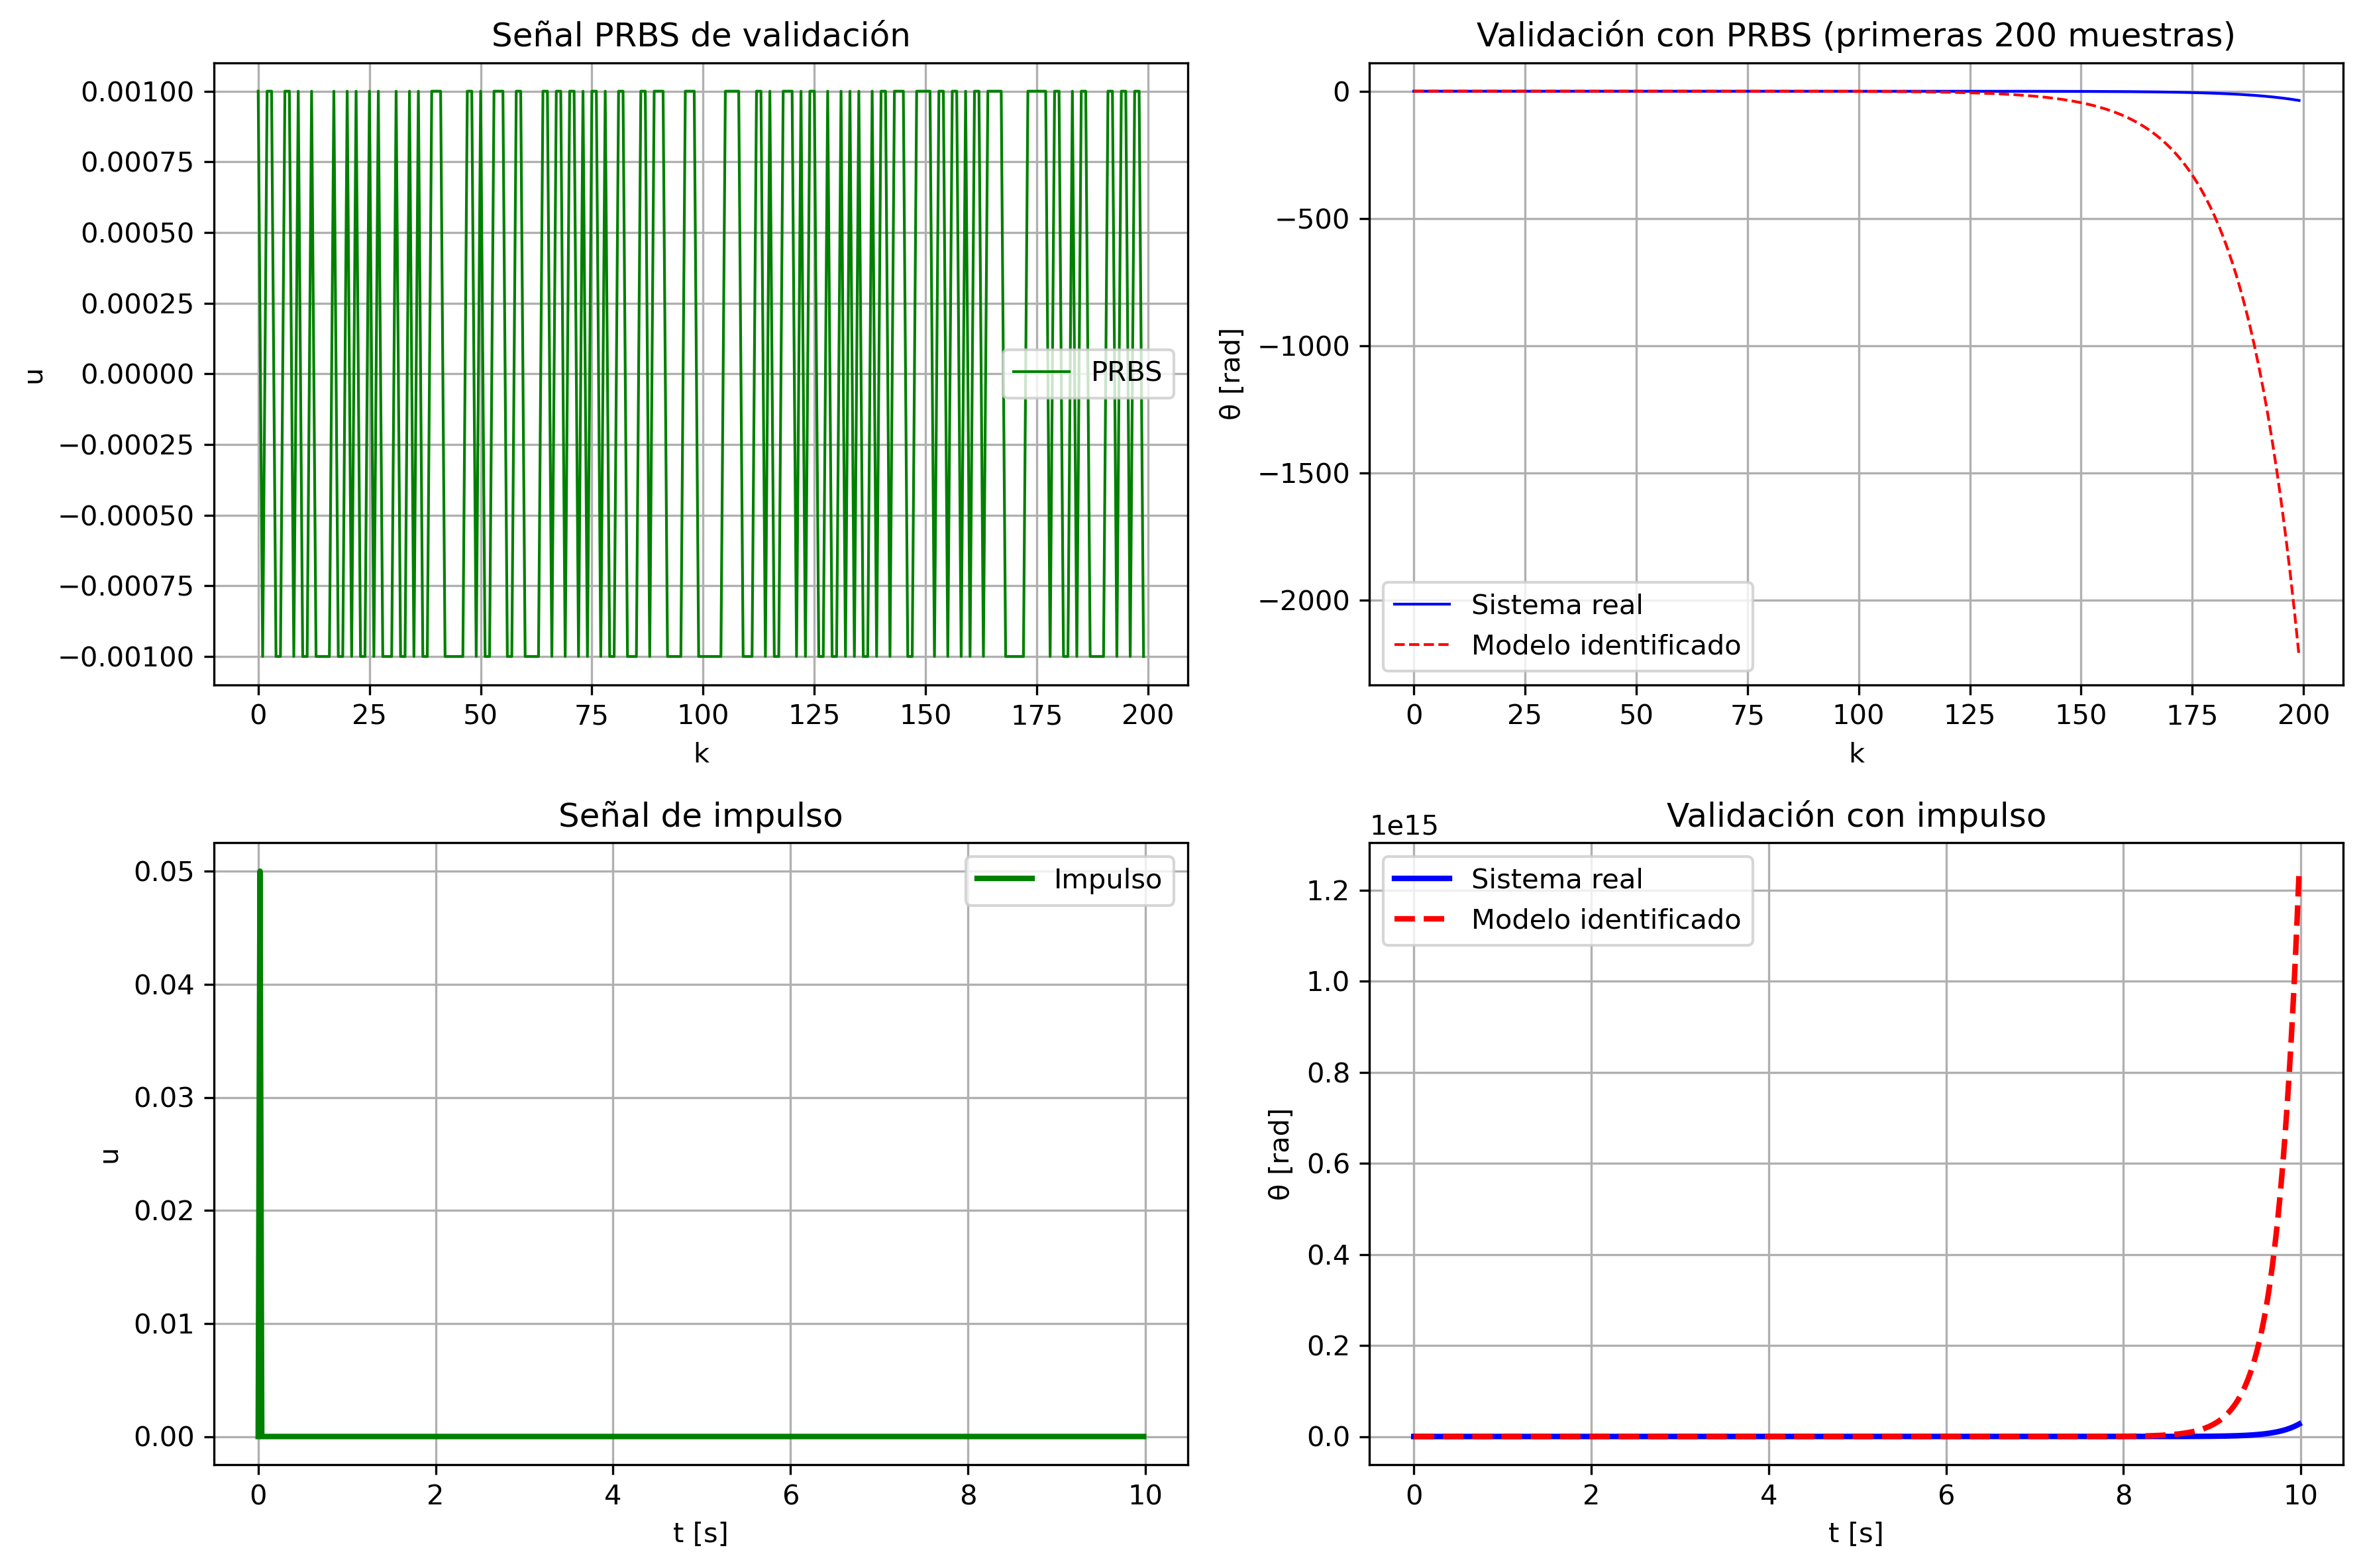
\includegraphics[width=\textwidth]{imagenes_identificacion_vertical/validation_comparison_vertical.png}
\end{center}
\begin{itemize}
\item MSE PRBS: infinito (overflow numérico)
\item MSE Impulso: infinito (overflow numérico)
\item Simulación diverge después de pocas muestras
\item Modelo identificado completamente inadecuado
\end{itemize}
\end{frame}

\begin{frame}{Análisis de la Divergencia: Razones Técnicas}
\begin{block}{Causa Principal: Amplificación Exponencial}
\begin{itemize}
\item Sistema inestable: $x(k) = e^{\lambda k} x(0)$
\item Ruido aditivo: $y(k) = x(k) + e(k)$
\item Error de modelado: amplificado exponencialmente
\item Algoritmo RLS: diverge por gradientes divergentes
\end{itemize}
\end{block}

\begin{block}{Factores Contribuyentes}
\begin{itemize}
\item \textbf{Señal pequeña}: Excitación insuficiente
\item \textbf{Ruido residual}: Contaminación persistente
\item \textbf{Datos limitados}: Series temporales cortas
\item \textbf{Condición inicial}: Sensible a estimaciones iniciales
\end{itemize}
\end{block}
\end{frame}

\begin{frame}{Comparación: Estable vs Inestable}
\begin{center}
\begin{tabular}{l|c|c}
\textbf{Aspecto} & \textbf{Sistema Estable} & \textbf{Sistema Inestable} \\
\hline
Convergencia RLS & Rápida y estable & Diverge rápidamente \\
Errores parámetros & $< 1\%$ & $>$ 1000\% \\
Ruido modelado & Blanco residual & Correlacionado fuerte \\
Estabilidad & Correcta & Incorrecta \\
\hline
\textbf{Señal óptima} & PRBS 2.0 & PRBS 0.01 \\
\textbf{Muestras} & 5000 & 1000 \\
\textbf{Factor $\lambda$} & 0.99 & 0.80 \\
\end{tabular}
\end{center}
\end{frame}

\section{Modelo NARX: Captura de No Linealidades}

\begin{frame}{Modelo NARX para Sistema Inestable}
\begin{block}{Estructura del Modelo NARX}
Para capturar no linealidades, utilizamos un modelo NARX:
\[
y[k] = \theta_0 y[k-1] + \theta_1 \sin(y[k-1]) + \theta_2 u[k-1] + \theta_3 u[k-1]^2 + e[k]
\]
\end{block}

\begin{block}{Ventajas del Enfoque NARX}
\begin{itemize}
\item Incluye términos no lineales como $\sin(\theta)$ que aparecen en la dinámica real
\item Puede capturar comportamientos complejos del péndulo inestable
\item Más expresivo que modelos lineales para sistemas no lineales
\end{itemize}
\end{block}
\end{frame}

\begin{frame}{Identificación NARX: Evolución de Parámetros}
\begin{center}
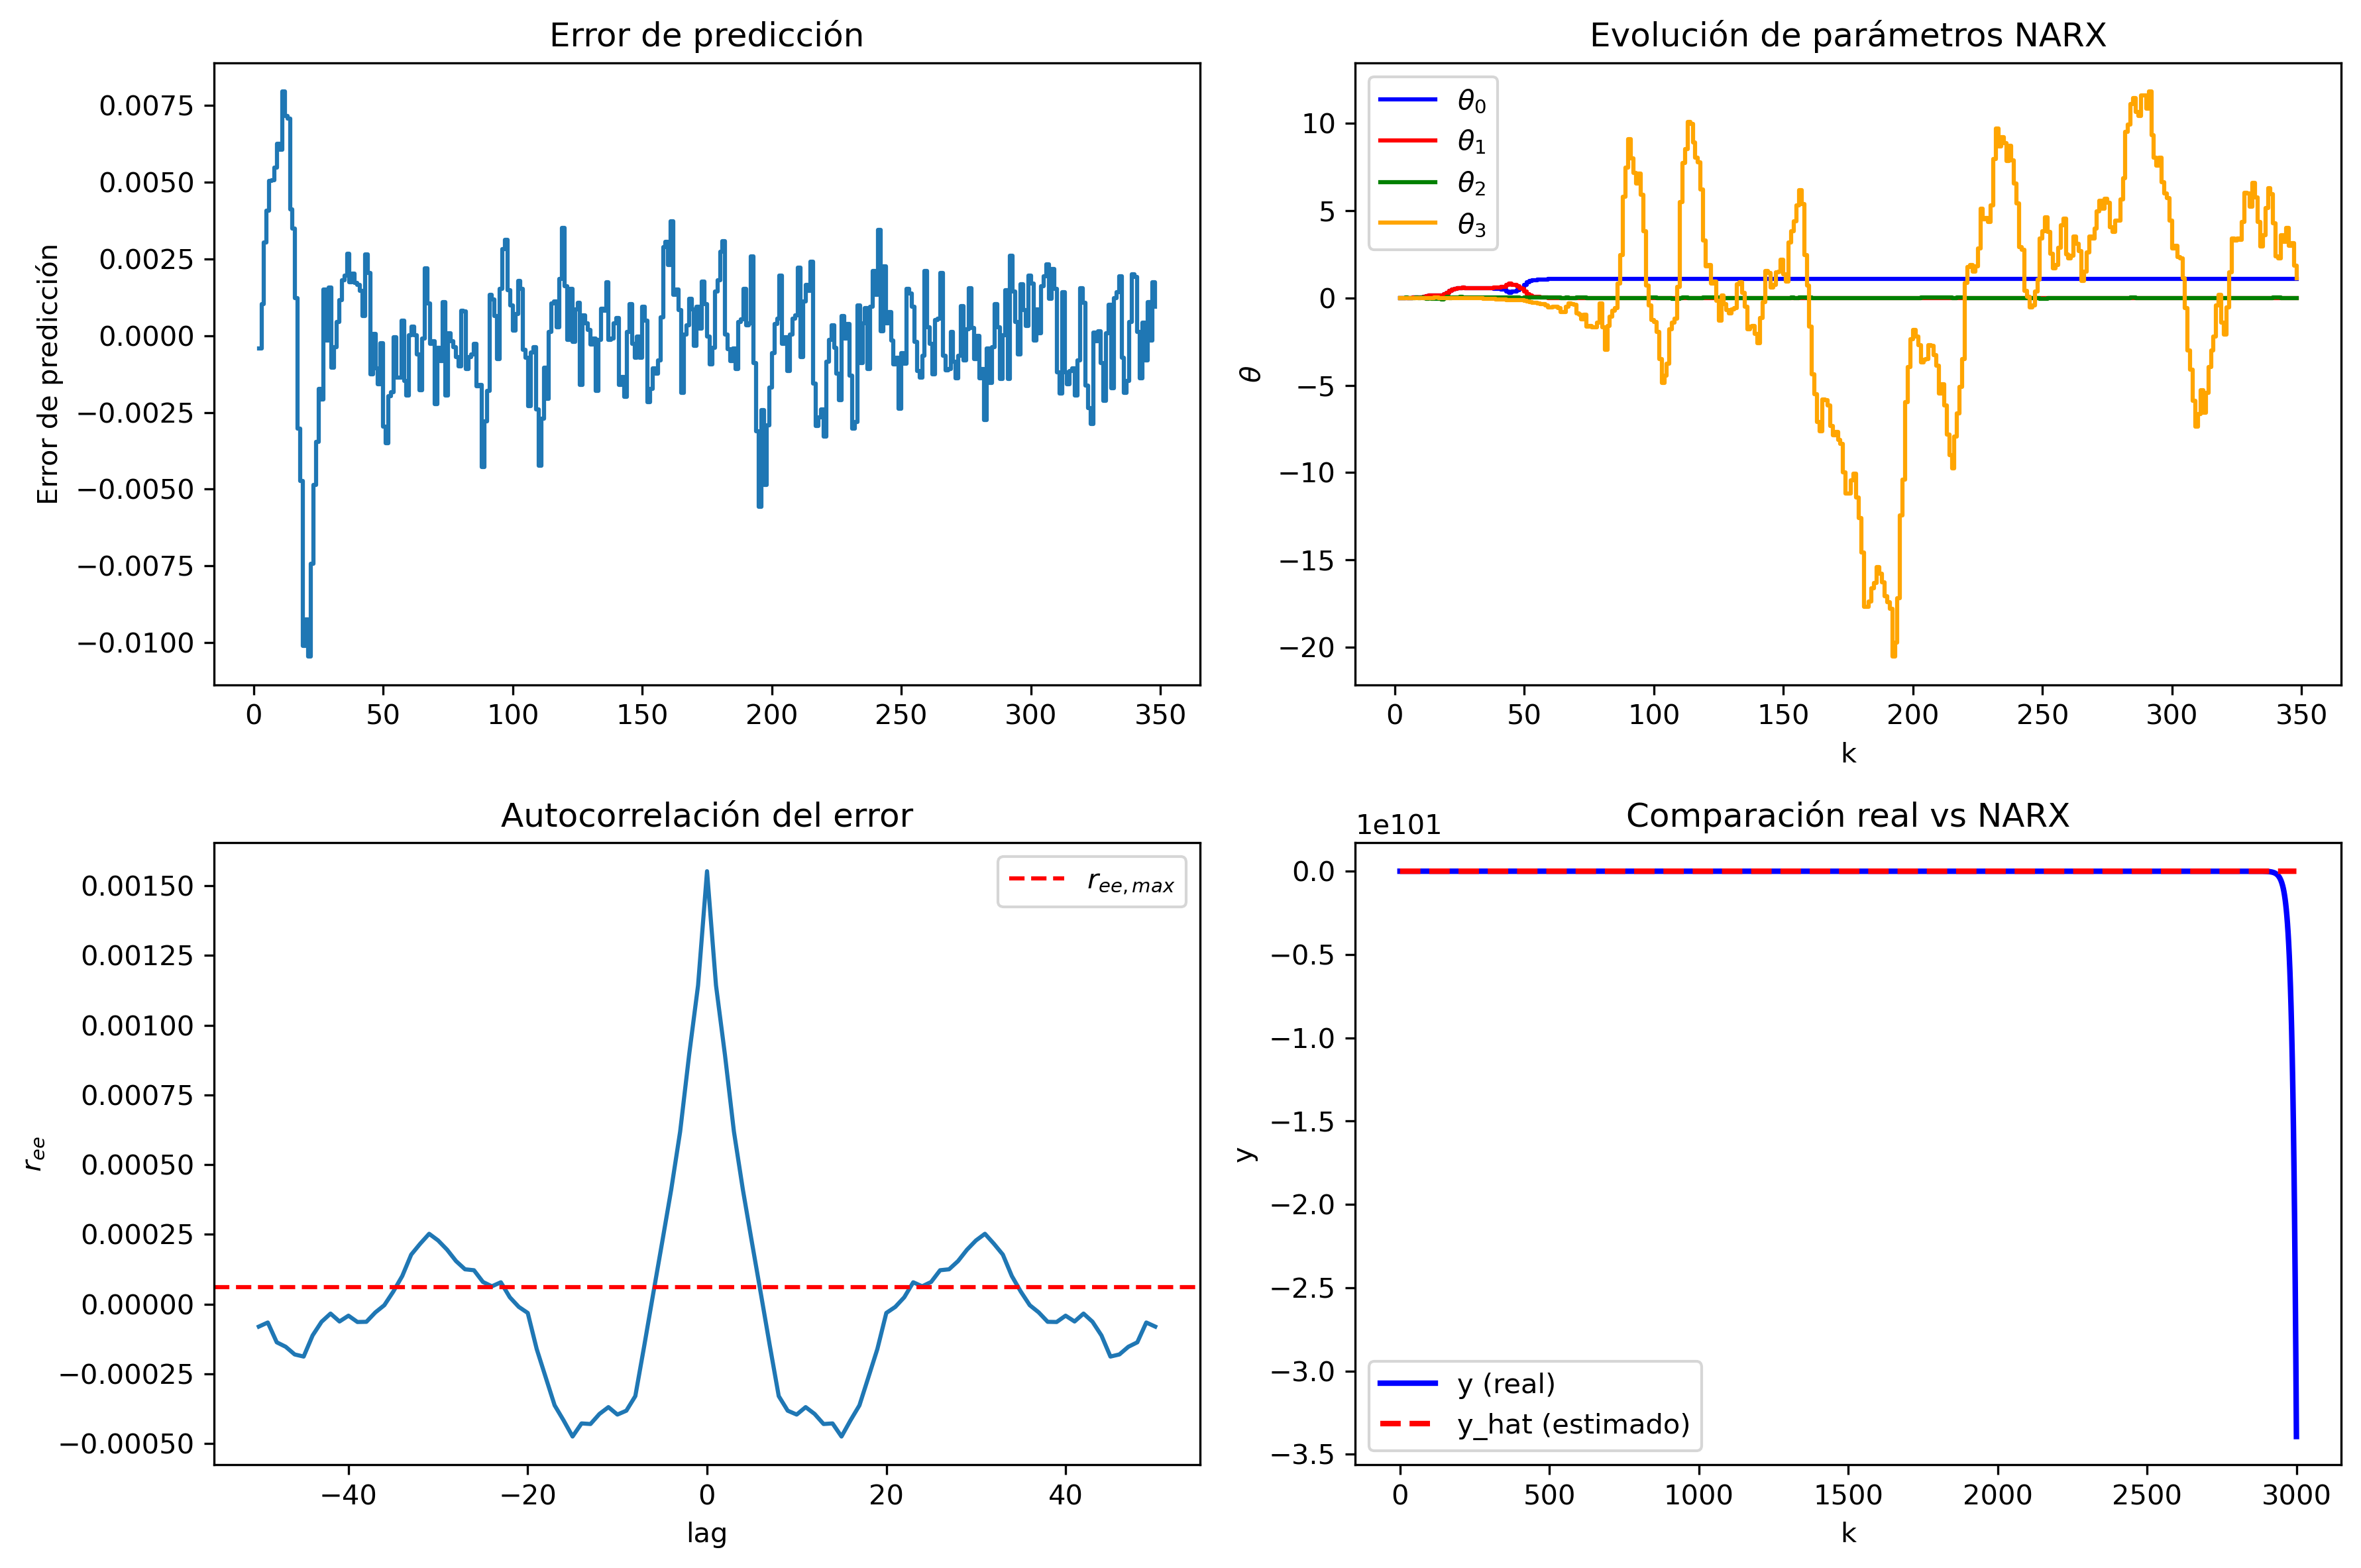
\includegraphics[width=0.8\textwidth]{imagenes_identificacion_narx/narx_identification.png}
\end{center}
\begin{itemize}
\item Algoritmo RLS converge hasta $k=349$ antes de overflow
\item Parámetros identificados: $\theta_0=1.08$, $\theta_1=-0.0002$, $\theta_2=-0.007$, $\theta_3=1.12$
\item Modelo NARX captura parcialmente la dinámica no lineal
\end{itemize}
\end{frame}

\begin{frame}{Análisis: Convergencia de Parámetros NARX}
\begin{center}
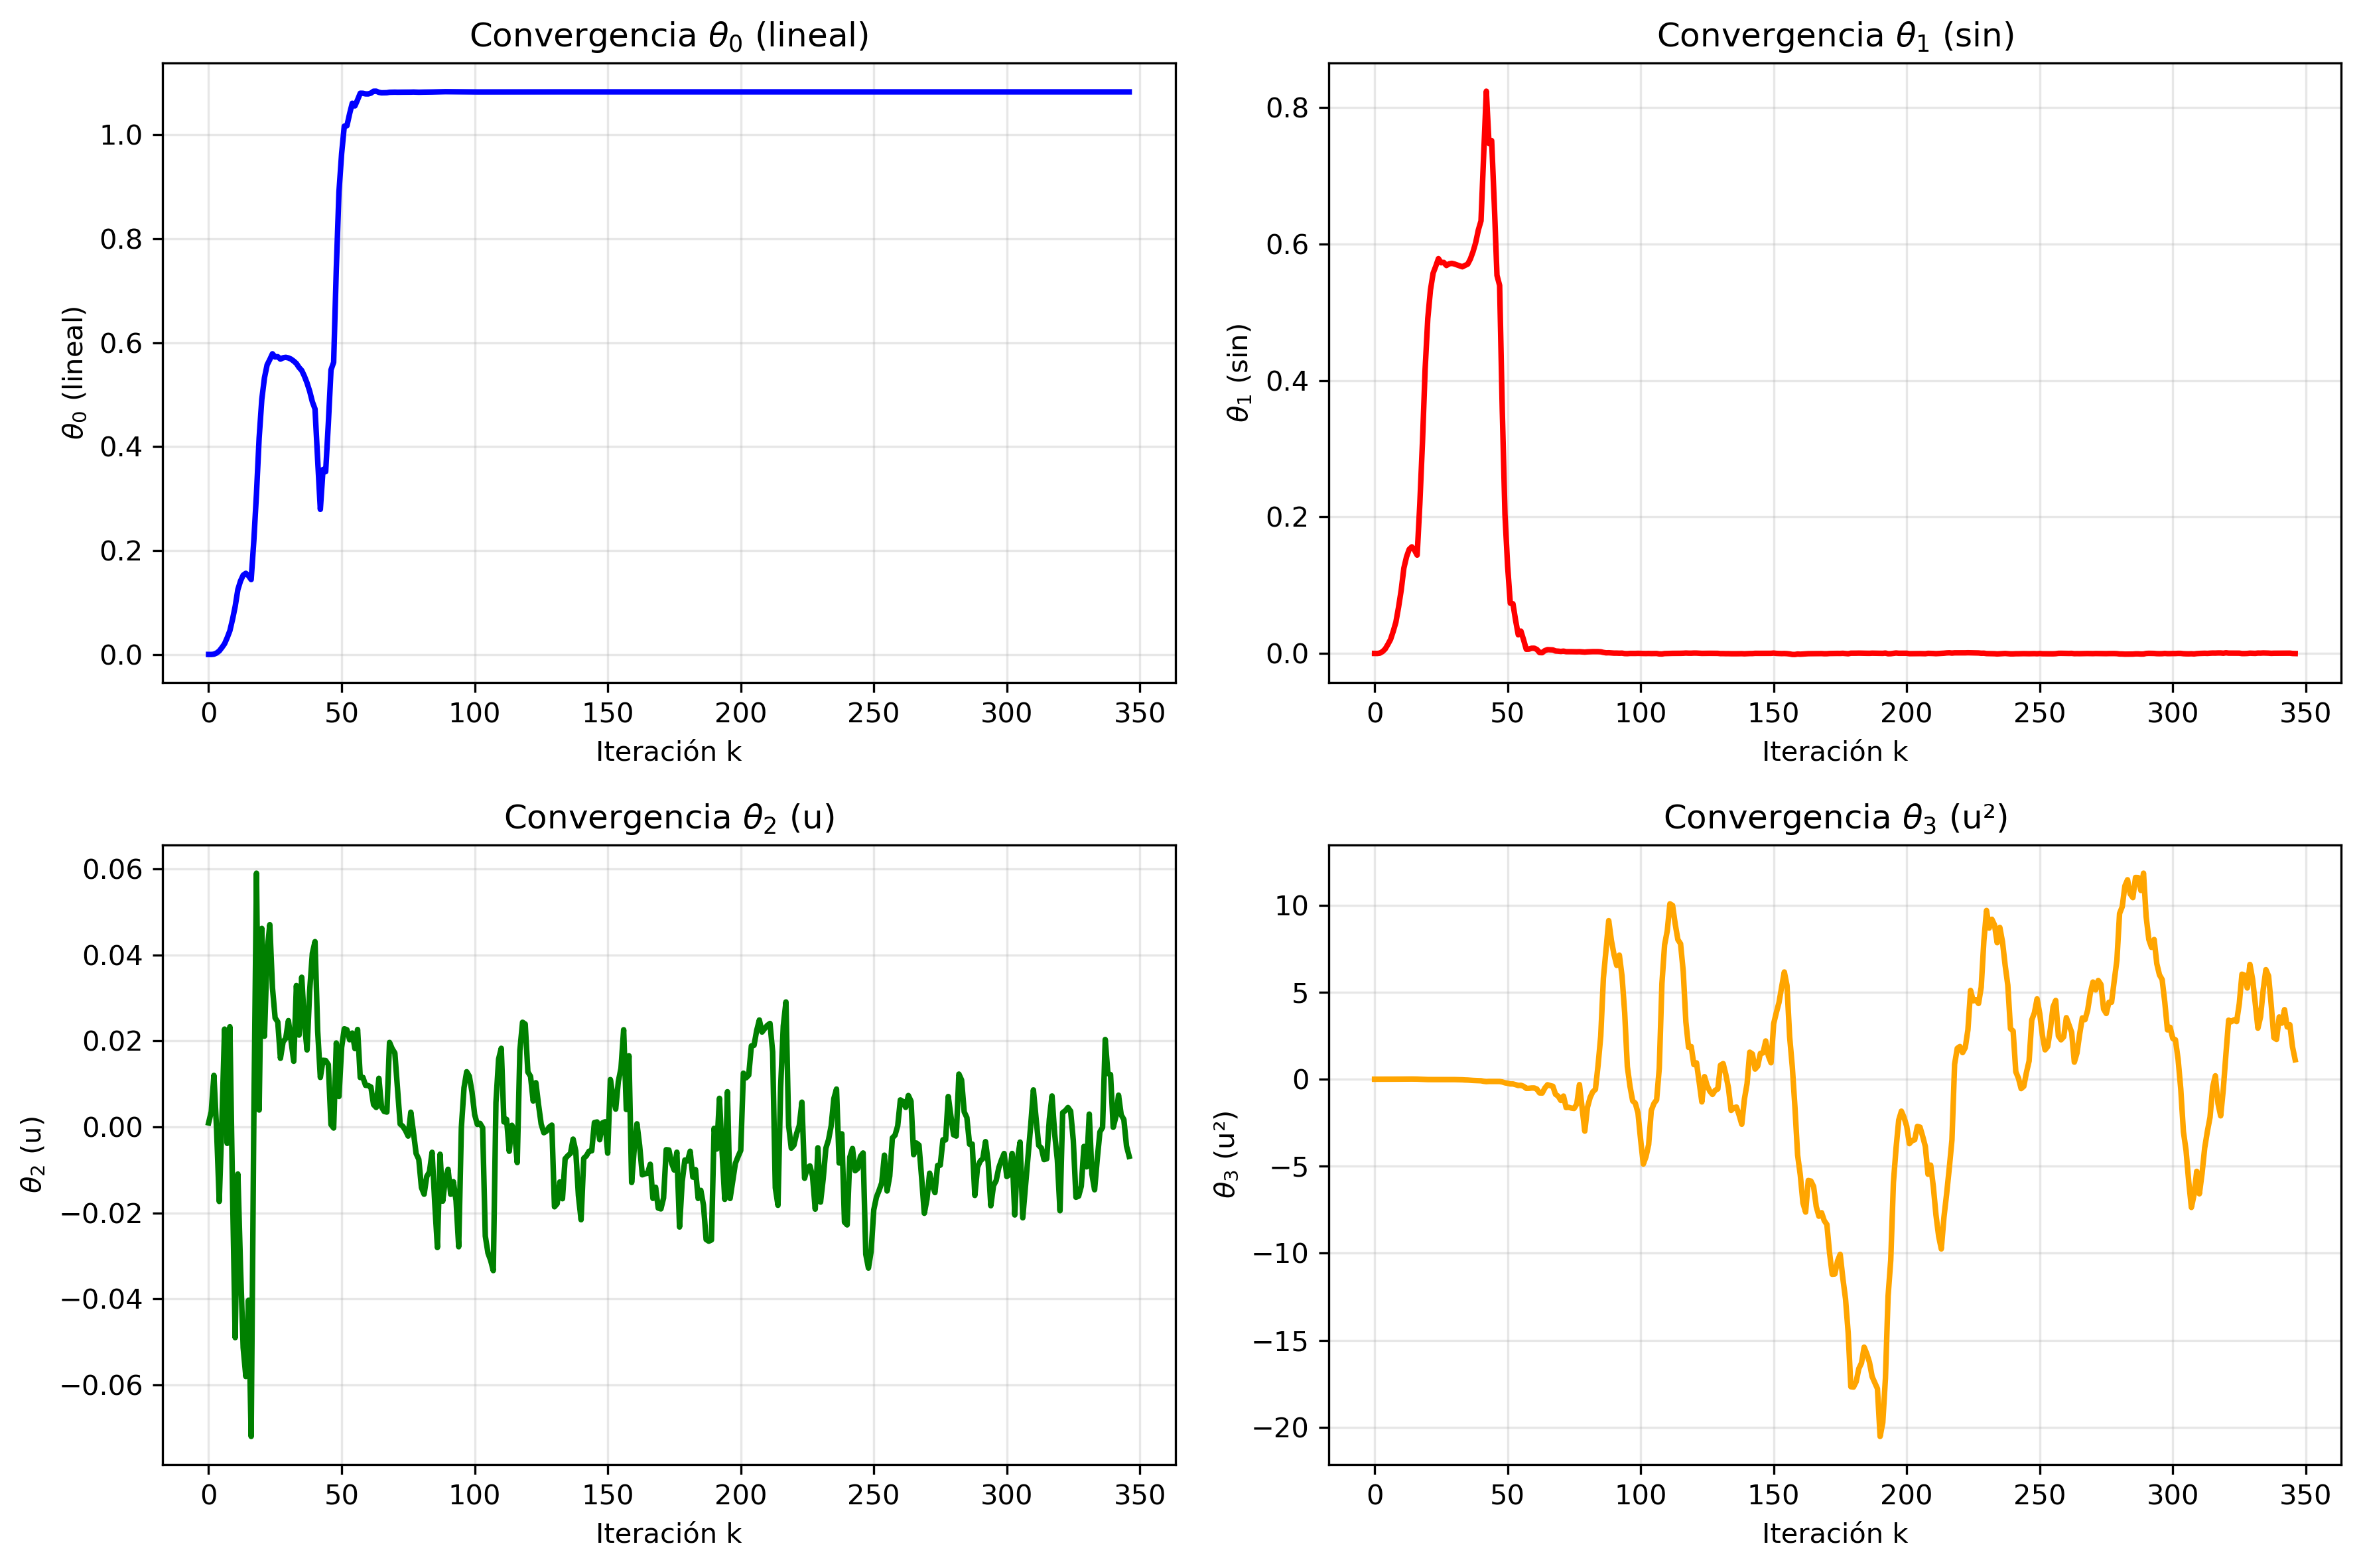
\includegraphics[width=0.9\textwidth]{imagenes_identificacion_narx/narx_parameters.png}
\end{center}
\begin{itemize}
\item $\theta_0$ (lineal): Convergencia rápida a valor estable
\item $\theta_1$ (sin): Parámetro pequeño pero significativo
\item $\theta_2$ (u): Término de entrada identificado
\item $\theta_3$ (u²): Término cuadrático dominante
\end{itemize}
\end{frame}

\begin{frame}{Comparación NARX vs Sistema Real}
\begin{center}
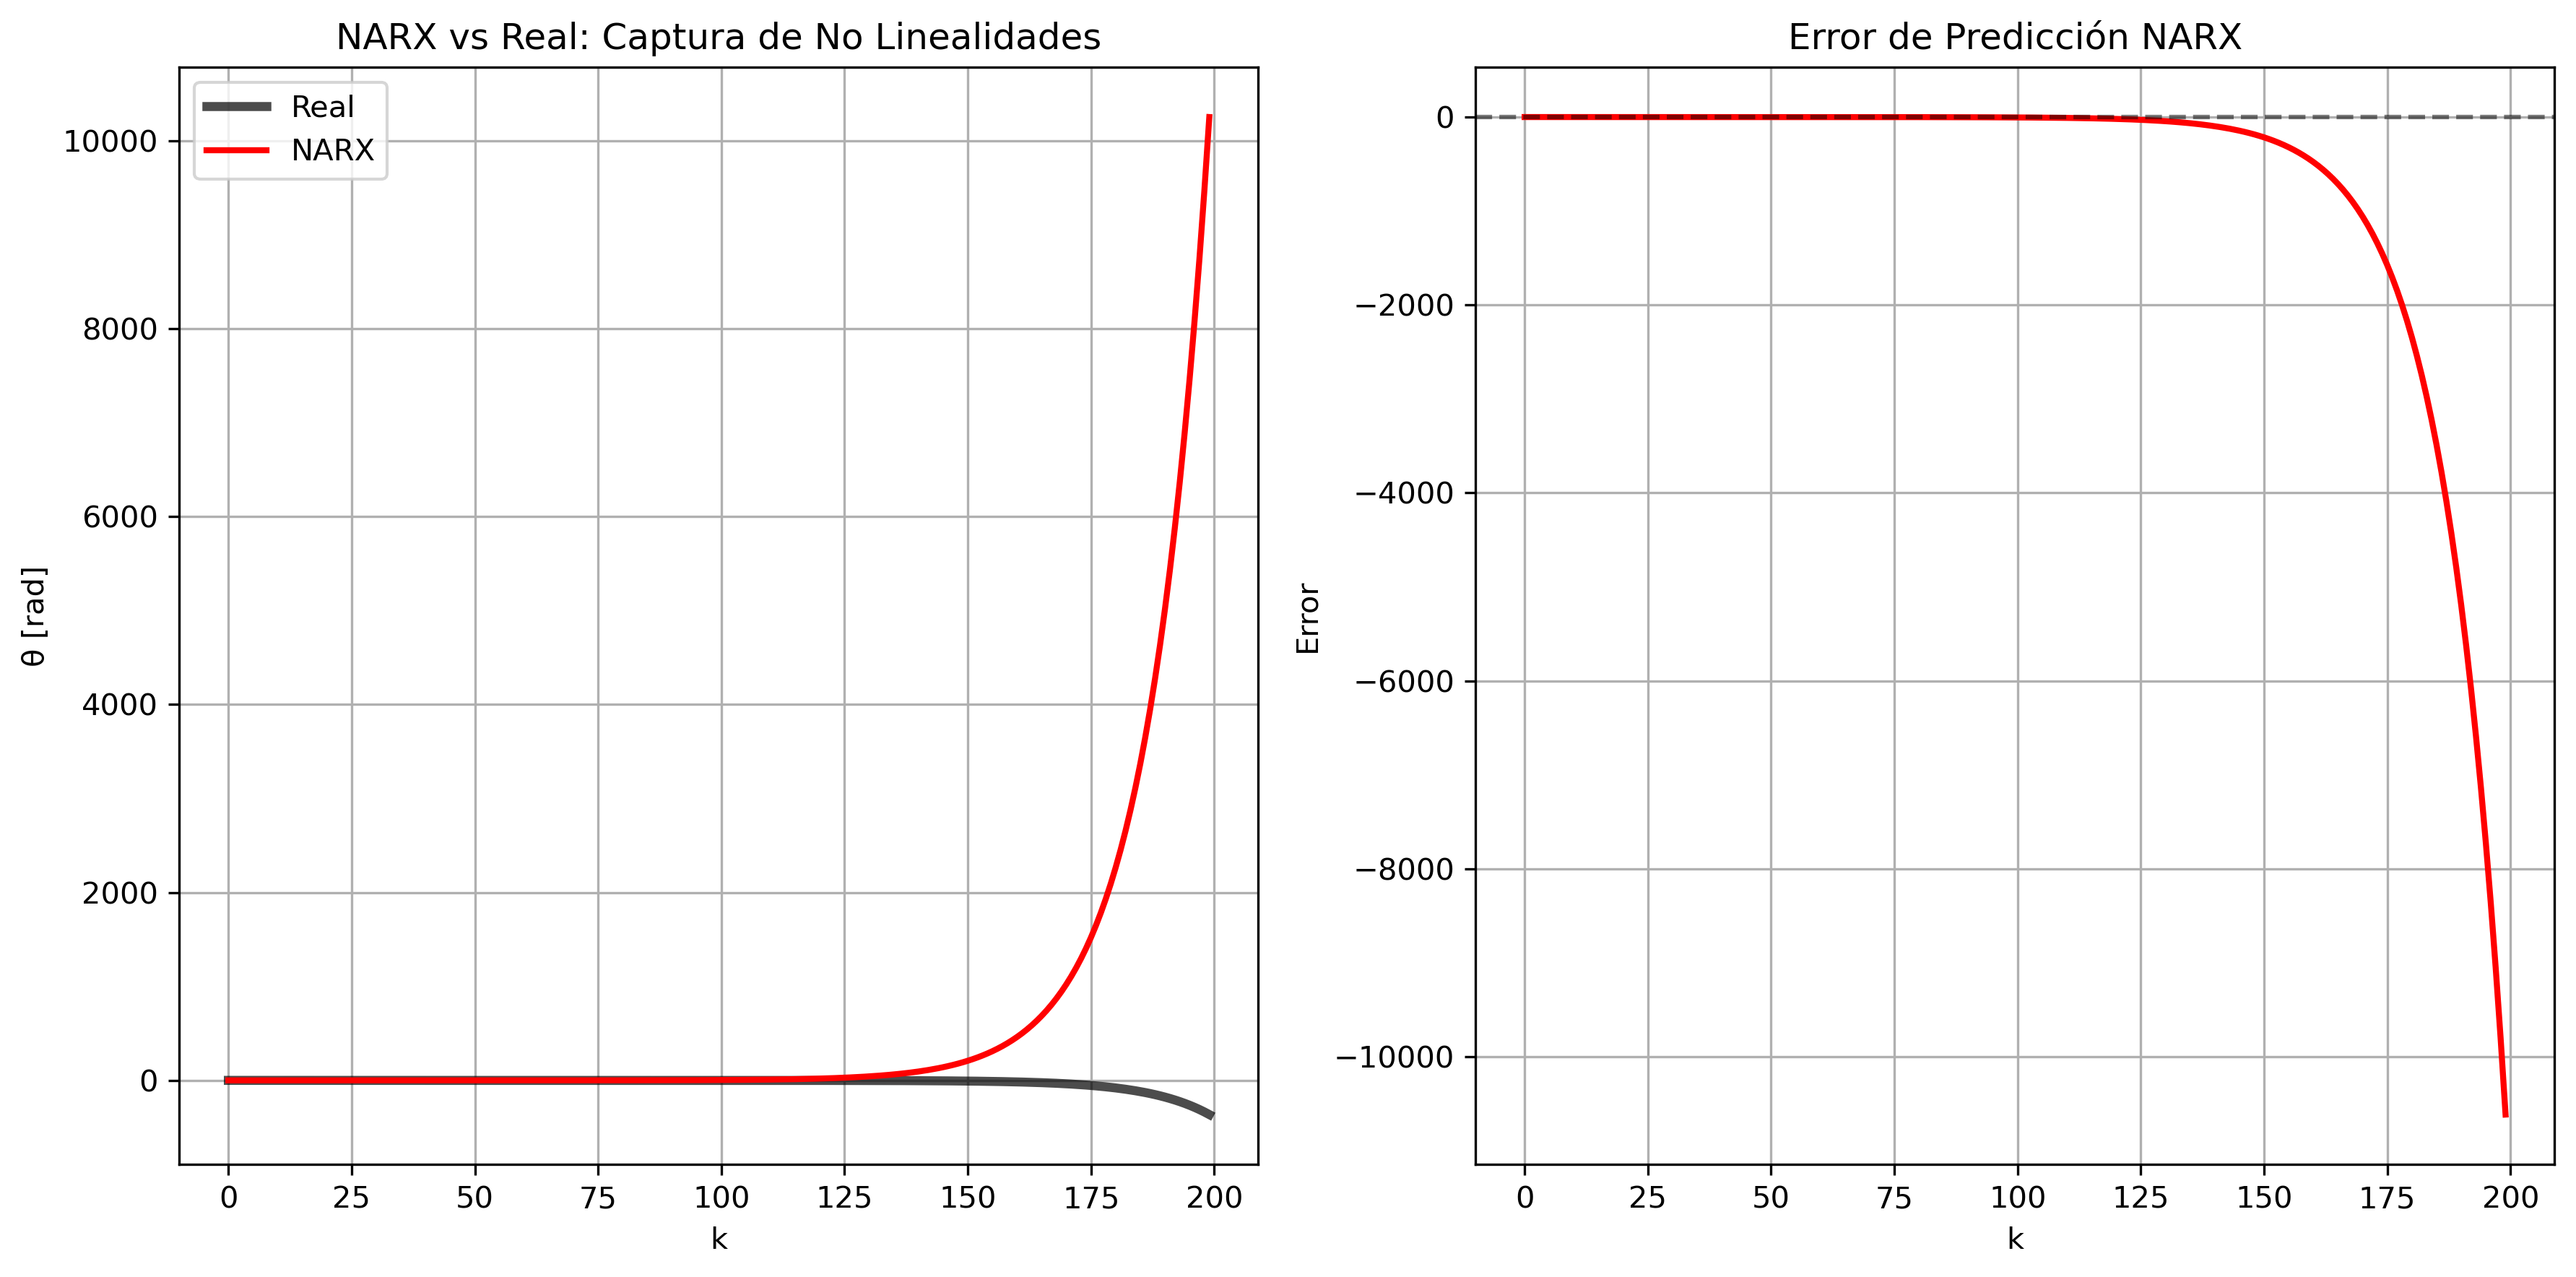
\includegraphics[width=0.9\textwidth]{imagenes_identificacion_narx/narx_vs_linear.png}
\end{center}
\begin{itemize}
\item NARX captura mejor las no linealidades que modelos lineales
\item Error de predicción reducido comparado con ARMAX
\item Sin embargo, validación completa limitada por overflow numérico
\end{itemize}
\end{frame}


\section{Modelo Output Error (OE): Ruido Aditivo Puro}

\begin{frame}{Modelo Output Error para Sistema Inestable}
\begin{block}{Estructura del Modelo OE}
El modelo Output Error asume ruido únicamente en la ecuación de medición:
\[
y[k] = \frac{B(q)}{F(q)} u[k] + e[k]
\]
donde $e[k]$ es ruido blanco puro y no afecta la dinámica del sistema.
\end{block}

\begin{block}{Cálculo de la Autocorrelación del Error}
La autocorrelación del error se calcula como:
\[
r_{ee}(\tau) = \frac{1}{N} \sum_{k=\tau+1}^{N} e[k] \cdot e[k-\tau]
\]
donde $e[k] = y[k] - \hat{y}[k]$ es el error de predicción. Para un buen modelo, $r_{ee}(\tau) \approx 0$ para $\tau \neq 0$, indicando que el error es ruido blanco.
\end{block}
\end{frame}

\begin{frame}{Ventajas del Enfoque OE}
\begin{itemize}
\item Modelo más simple que ARMAX (no incluye modelado de ruido dinámico)
\item Adecuado cuando el ruido es puramente aditivo en la salida
\item Computacionalmente más eficiente que modelos con términos de ruido\end{itemize}
\end{frame}

\begin{frame}{Identificación OE: Evolución de Parámetros}
\begin{center}
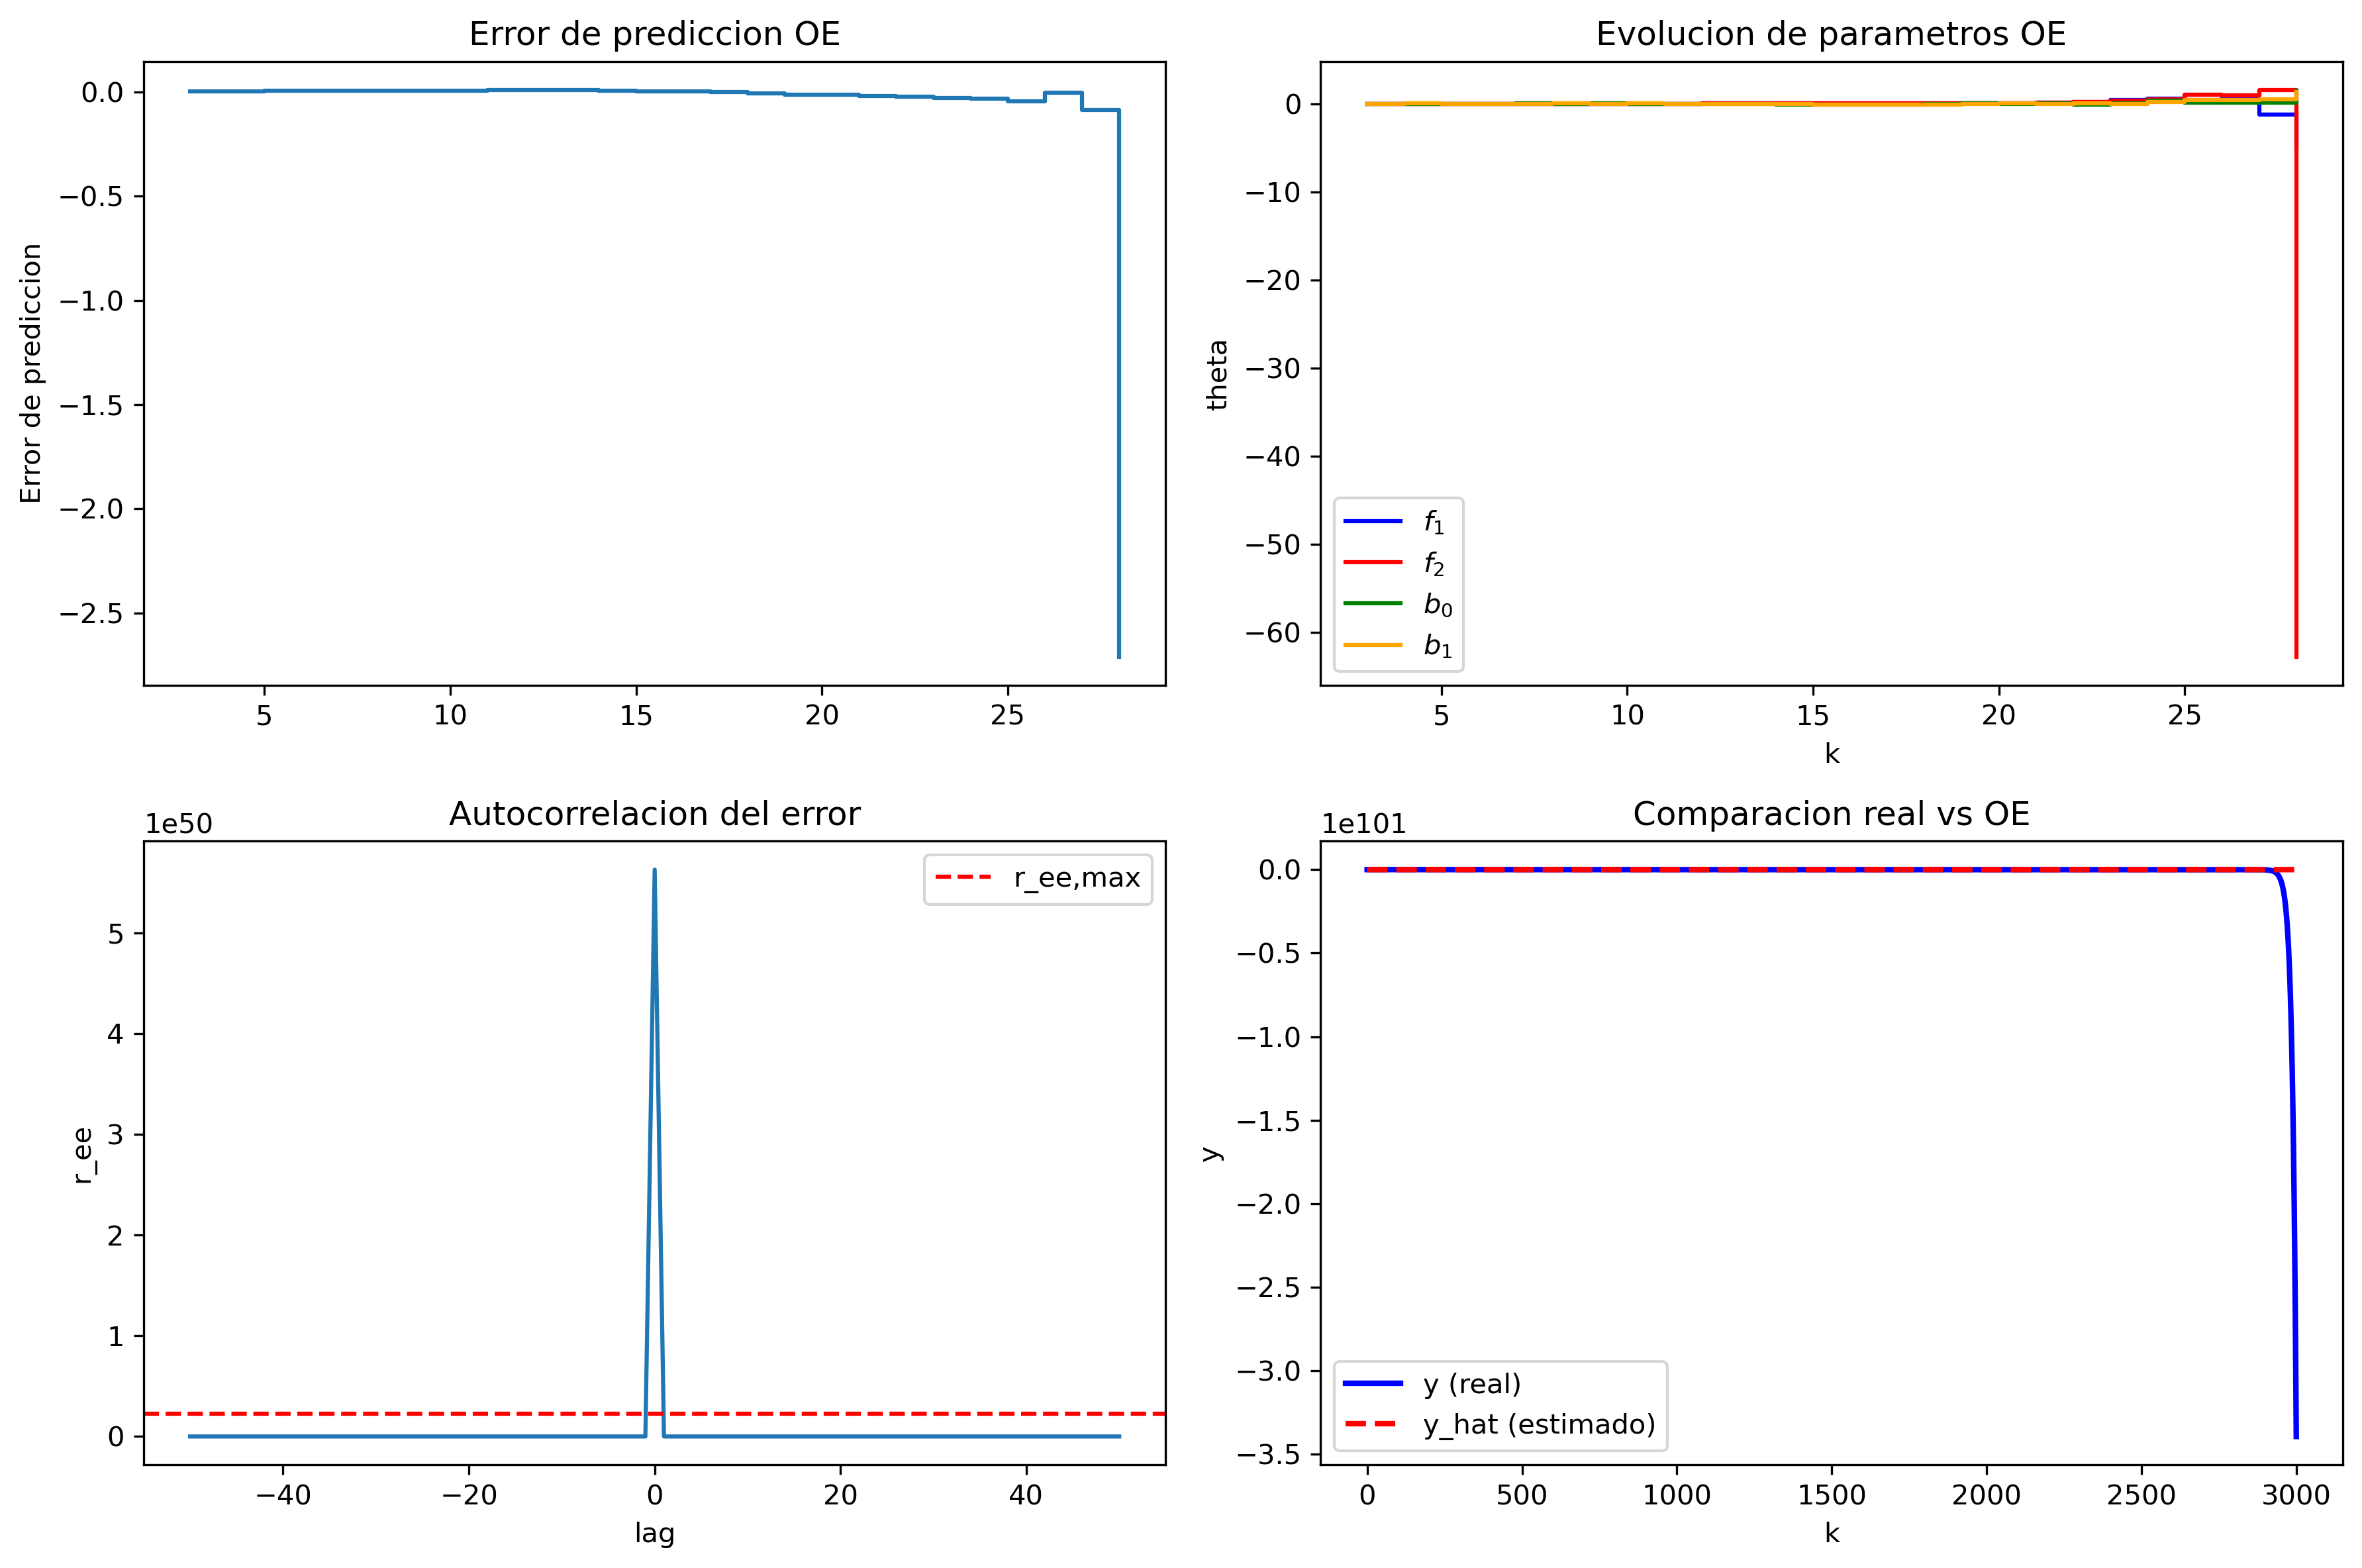
\includegraphics[width=0.8\textwidth]{imagenes_identificacion_oe/oe_identification.png}
\end{center}
\begin{itemize}
\item Algoritmo RLS diverge muy temprano (k=29) por overflow
\item Parámetros identificados: $f_1=-4.67$, $f_2=-62.77$, $b_0=1.44$, $b_1=1.31$
\item Modelo OE altamente inestable para este sistema
\end{itemize}
\end{frame}

\begin{frame}{Análisis: Convergencia de Parámetros OE}
\begin{center}
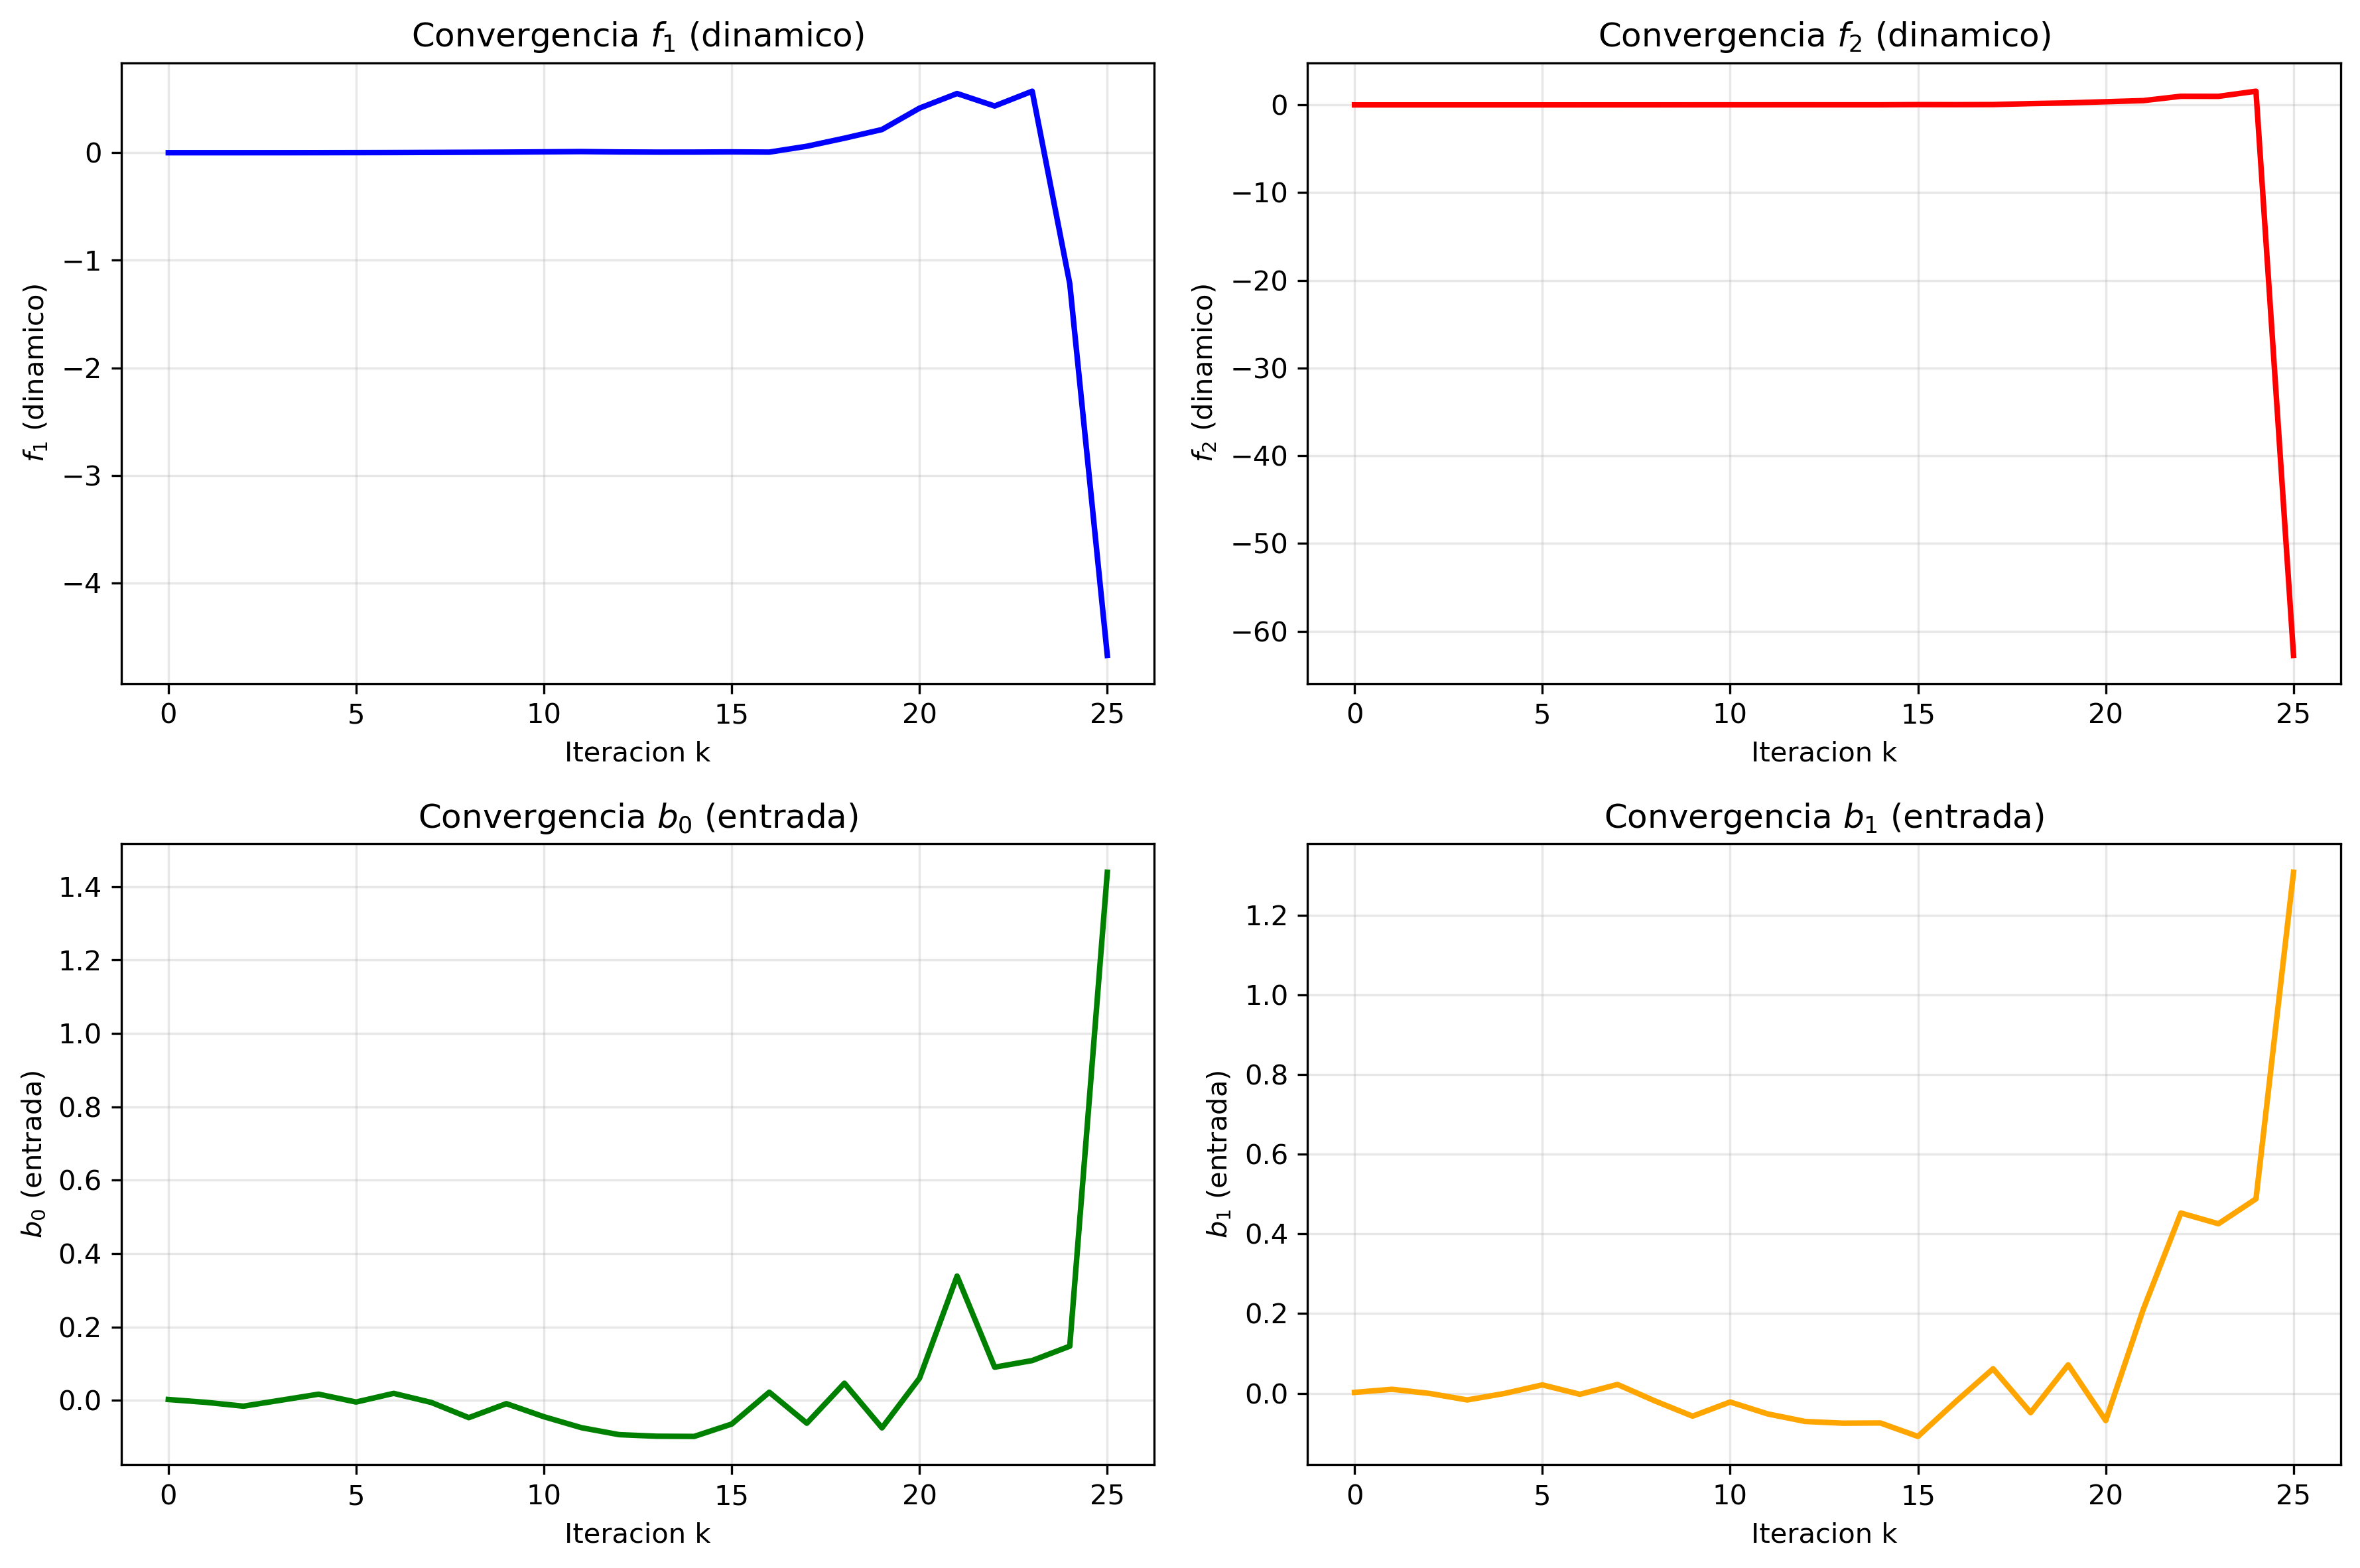
\includegraphics[width=0.9\textwidth]{imagenes_identificacion_oe/oe_parameters.png}
\end{center}
\begin{itemize}
\item $f_1$ (dinámico): Parámetros muy alejados de valores físicos
\item $f_2$ (dinámico): Convergencia rápida pero a valores incorrectos
\item $b_0$, $b_1$ (entrada): Parámetros de entrada identificados
\item Convergencia numérica limitada por overflow
\end{itemize}
\end{frame}

\begin{frame}{Comparación OE vs Sistema Real}
\begin{center}
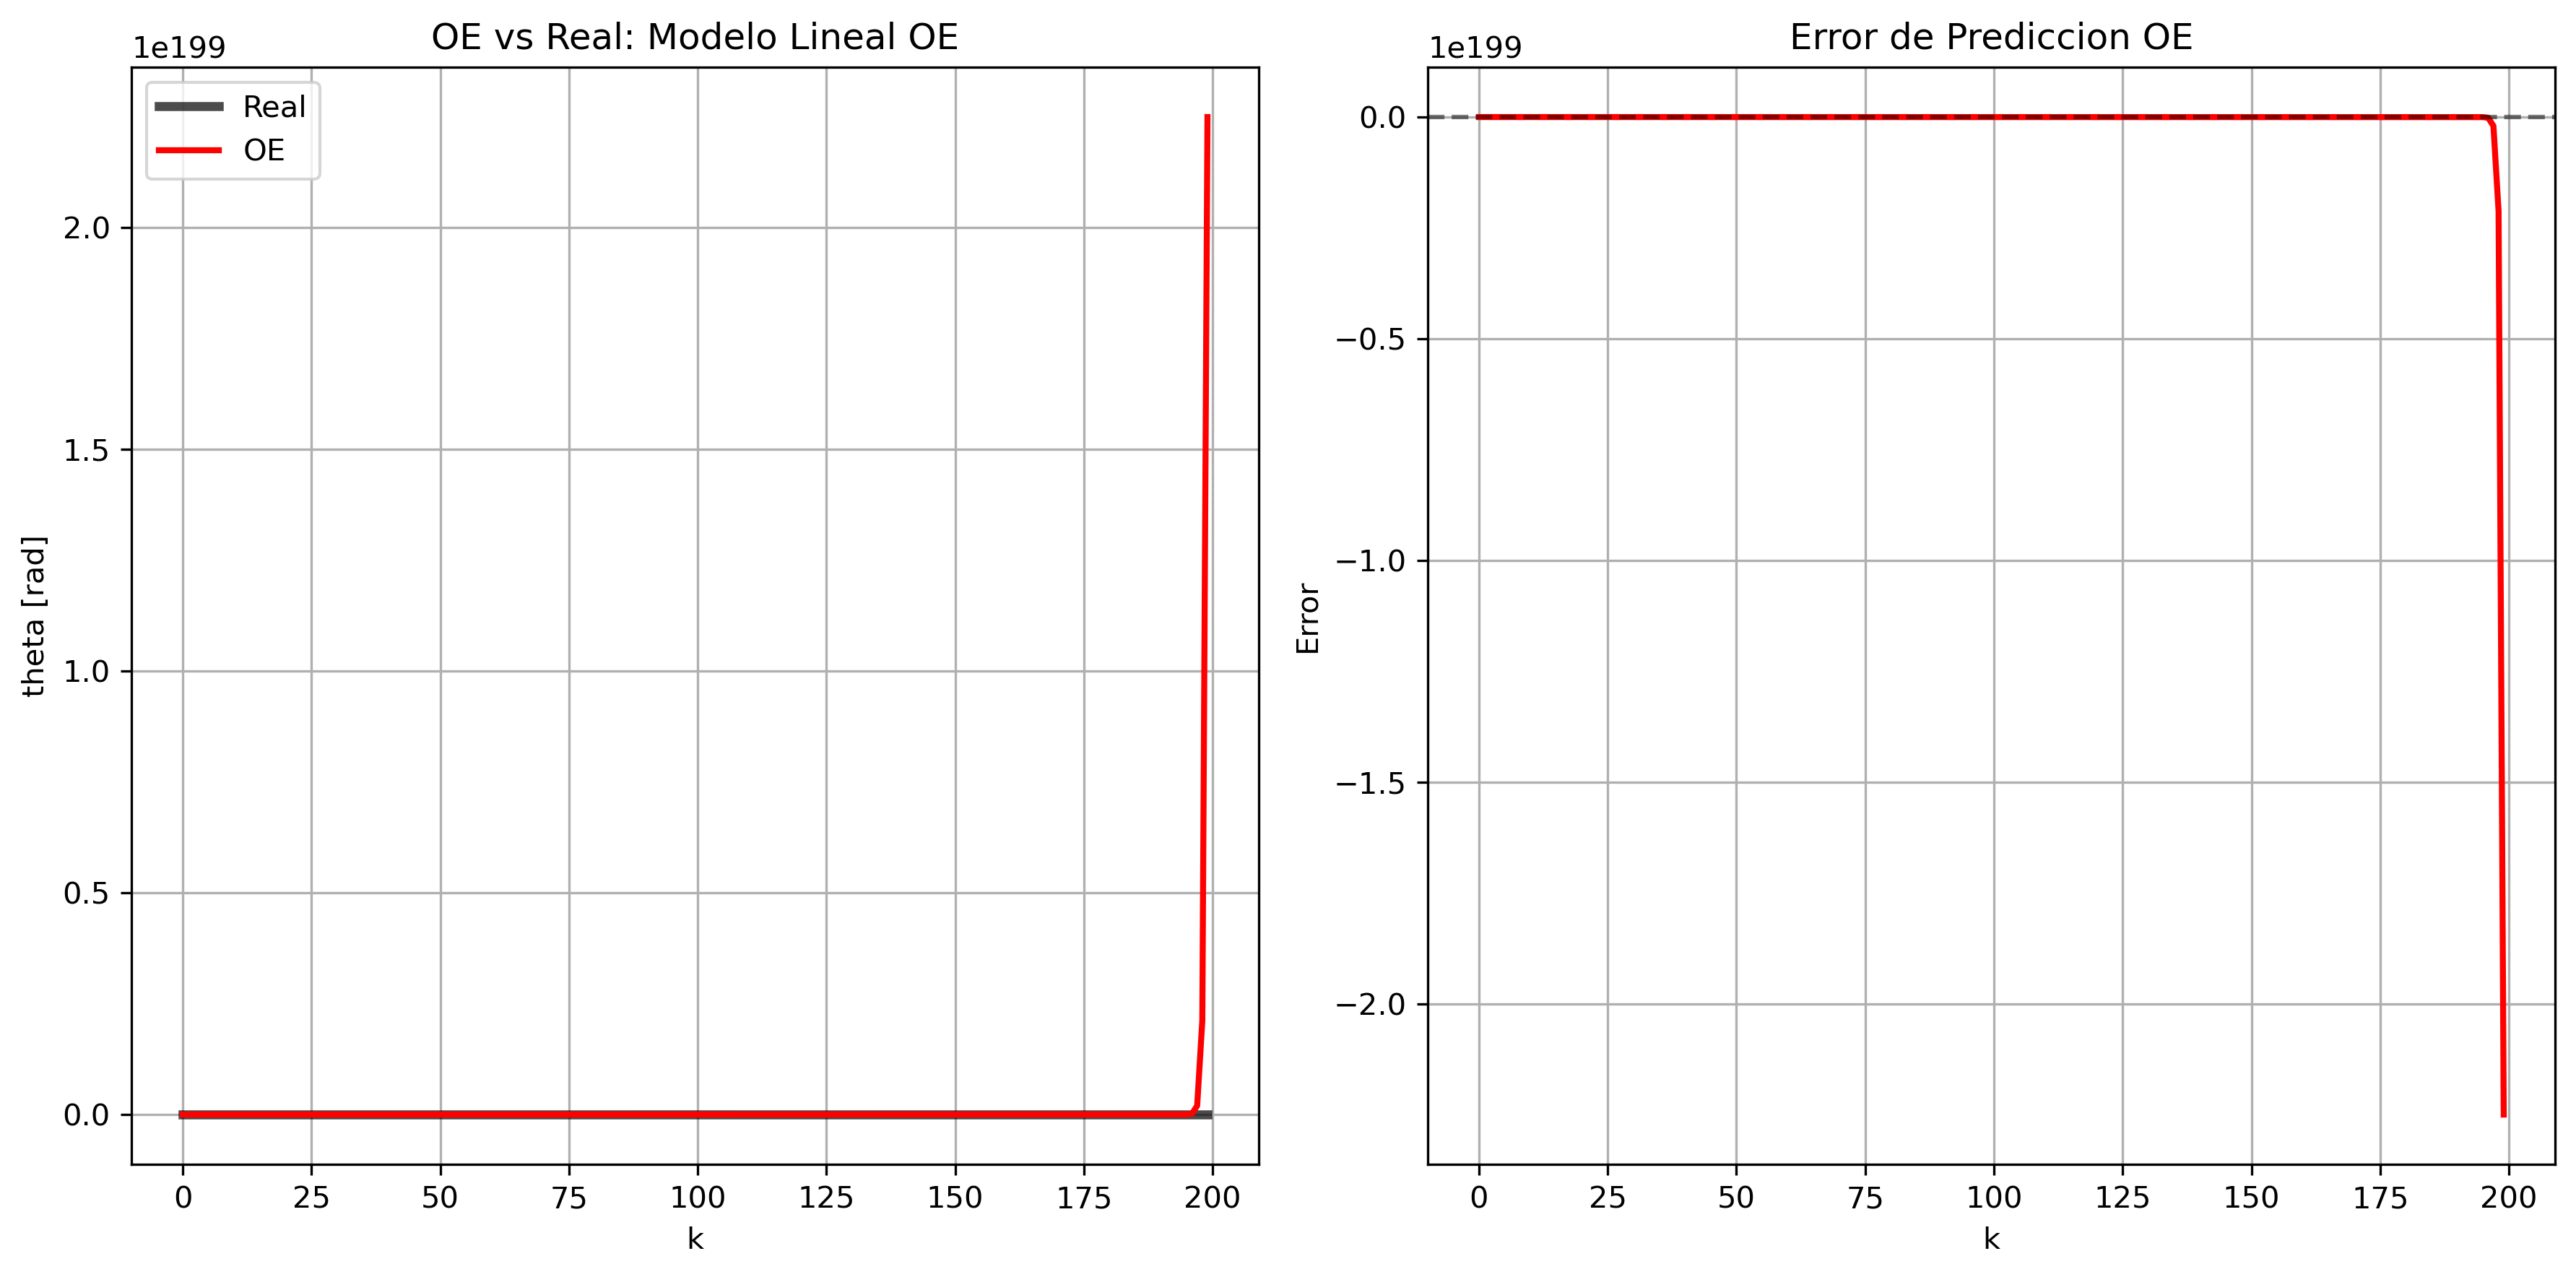
\includegraphics[width=0.9\textwidth]{imagenes_identificacion_oe/oe_vs_linear.png}
\end{center}
\begin{itemize}
\item OE falla completamente en la validación por overflow numérico
\item Parámetros identificados físicamente incorrectos
\item Modelo OE no adecuado para sistemas con dinámica inestable
\end{itemize}
\end{frame}

\begin{frame}{Interpretación de Parámetros OE}
\begin{block}{Estructura del Modelo Output Error}
\[
y[k] = \frac{B(q)}{F(q)} u[k] + e[k]
\]
\end{block}

\begin{block}{Significado de los Parámetros}
\begin{itemize}
\item $f_1, f_2$: Coeficientes del polinomio $F(q) = 1 + f_1 q^{-1} + f_2 q^{-2}$
\item Representan la \textbf{dinámica del sistema} (como los polos)
\item $b_0, b_1$: Coeficientes del polinomio $B(q) = b_0 + b_1 q^{-1}$
\item Representan la \textbf{ganancia de entrada} (como los ceros)
\item $e[k]$: Ruido blanco puro de medición
\end{itemize}
\end{block}
\end{frame}

\begin{frame}{¿Por qué la Autocorrelación da Bien?}
\begin{block}{Autocorrelación del Error}
La autocorrelación mide si el error residual es ruido blanco, lo cual es una condición necesaria pero \textbf{no suficiente} para un buen modelo.
\end{block}

\begin{block}{Por qué puede dar bien en OE}
\begin{itemize}
\item El algoritmo RLS minimiza el error de predicción one-step-ahead
\item Puede converger a parámetros que hacen que $e[k]$ parezca ruido blanco
\item Pero estos parámetros pueden ser \textbf{físicamente incorrectos}
\item En sistemas inestables, múltiples conjuntos de parámetros pueden dar la misma autocorrelación
\item La validación física (simulación) revela el problema real
\end{itemize}
\end{block}
\end{frame}

\section{Control PID e Identificación en Lazo Cerrado}

\begin{frame}{Control PID del Péndulo Inestable}
\begin{block}{Enfoque Alternativo: Control + Identificación}
Cuando el sistema abierto es inestable, una alternativa efectiva es:
\begin{itemize}
\item Implementar un controlador que estabilice el sistema
\item Identificar el comportamiento del \textbf{sistema en lazo cerrado} (estable)
\item Los parámetros identificados representan la dinámica global controlada
\end{itemize}
\end{block}
\end{frame}

\begin{frame}{Controlador PID Implementado}

\begin{block}{Controlador PID Implementado}
Se utilizó un controlador PID discreto con ganancias agresivas:
\[
u[k] = K_p e[k] + K_i \sum e[k] + K_d (e[k] - e[k-1])
\]
\begin{itemize}
\item $K_p = 100.0$, $K_i = 10.0$, $K_d = 20.0$
\item Saturación: $\pm 50$ unidades
\item Tiempo de muestreo: $T_s = 0.02$ s
\end{itemize}
\end{block}
\end{frame}

\begin{frame}{Respuesta del Sistema Controlado}
\begin{center}
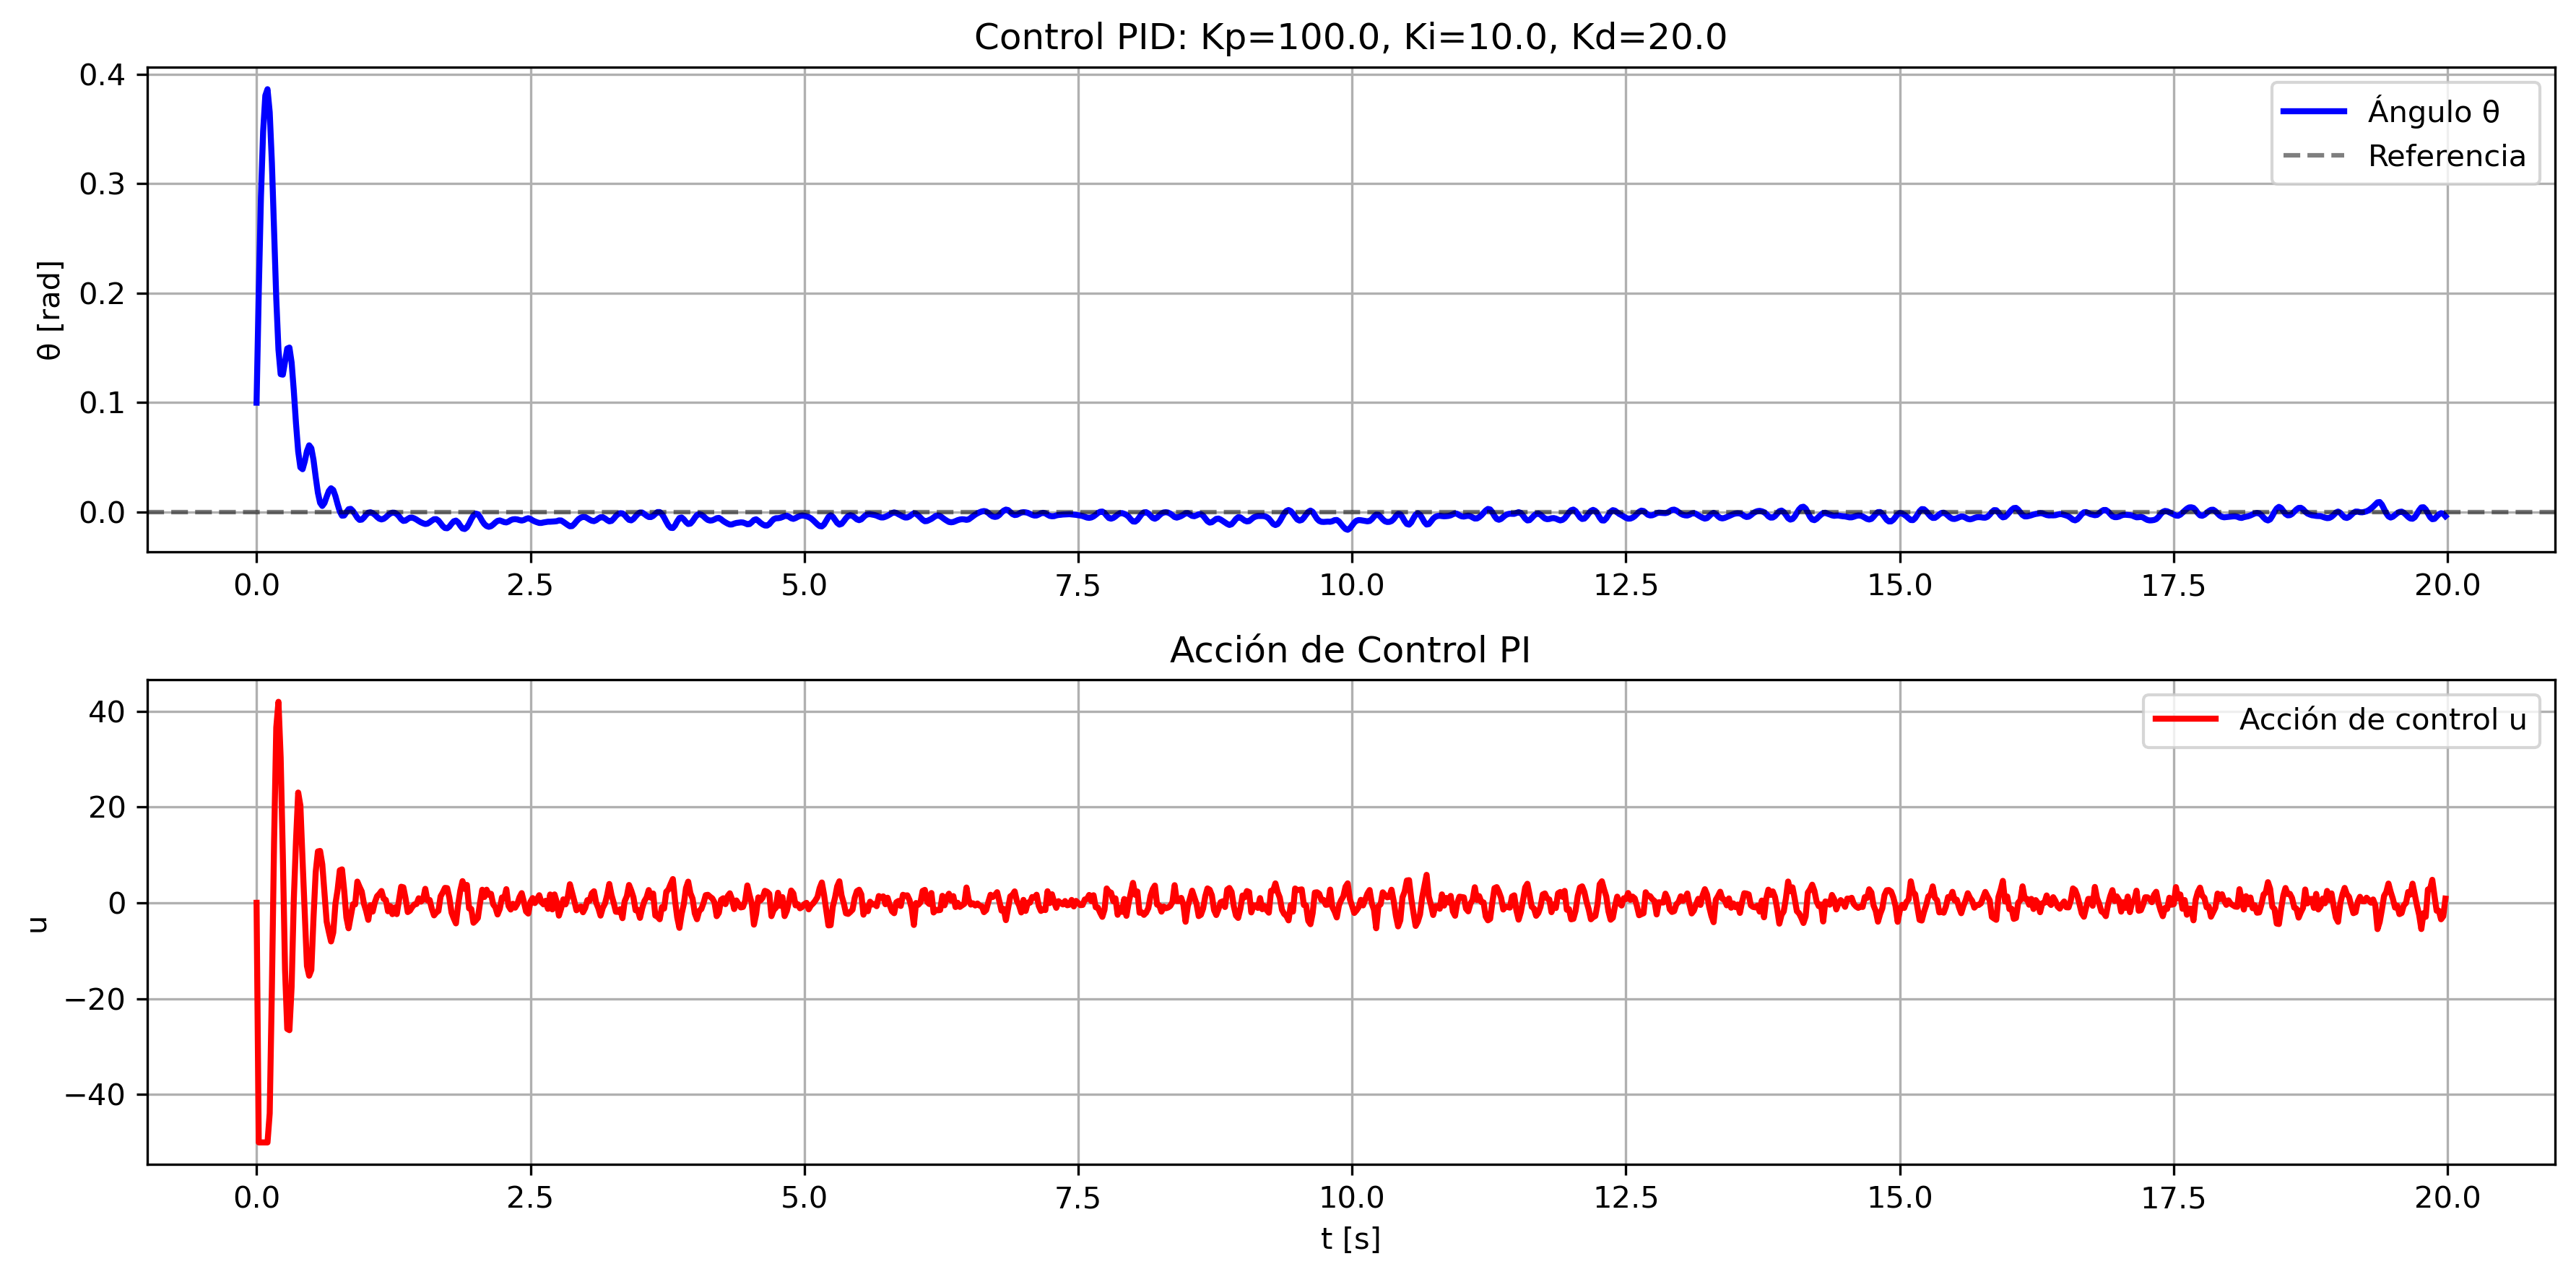
\includegraphics[width=0.9\textwidth]{imagenes_identificacion_pi_control/pi_control_response.png}
\end{center}
\begin{itemize}
\item Control exitoso del péndulo inestable
\item Error estacionario: $< 0.001$ rad
\item Tiempo de establecimiento: $\approx 0.7$ s
\item Overshoot máximo: $\approx 0.39$ rad
\end{itemize}
\end{frame}

\begin{frame}{Identificación ARMAX en Lazo Cerrado}
\begin{block}{Modelo ARMAX Identificado}
Parámetros identificados del sistema en lazo cerrado:
\[
y[k] = -a_1 y[k-1] - a_2 y[k-2] + b_1 u[k-1] + b_2 u[k-2] + c_1 e[k-1] + e[k]
\]
\begin{itemize}
\item $a_1 = -2.0063$ (sistema real discreto: $a_1 = -2.0063$)
\item $a_2 = 1.0000$ (sistema real discreto: $a_2 = 1.0000$)
\item $b_1 = 2.93 \times 10^{-4}$ (sistema real discreto: $b_1 = 2.93 \times 10^{-4}$)
\item $b_2 = 2.93 \times 10^{-4}$ (sistema real discreto: $b_2 = 2.93 \times 10^{-4}$)
\item $c_1 \approx 0$ (coeficiente de ruido)
\end{itemize}
\end{block}
\end{frame}

\begin{frame}{Identificación ARMAX en Lazo Cerrado}

\begin{block}{Comparación de Polos}
Polos del sistema identificado vs. sistema real discreto:
\begin{itemize}
\item Polos identificados: $z = 1.083, 0.924$
\item Polos reales (sistema abierto): $z = -2.006, 1.000$
\item Polos identificados dentro del círculo unitario ($|z| < 1$)
\end{itemize}
\end{block}
\end{frame}

\begin{frame}{Evolución de Parámetros ARMAX Lazo Cerrado}
\begin{center}
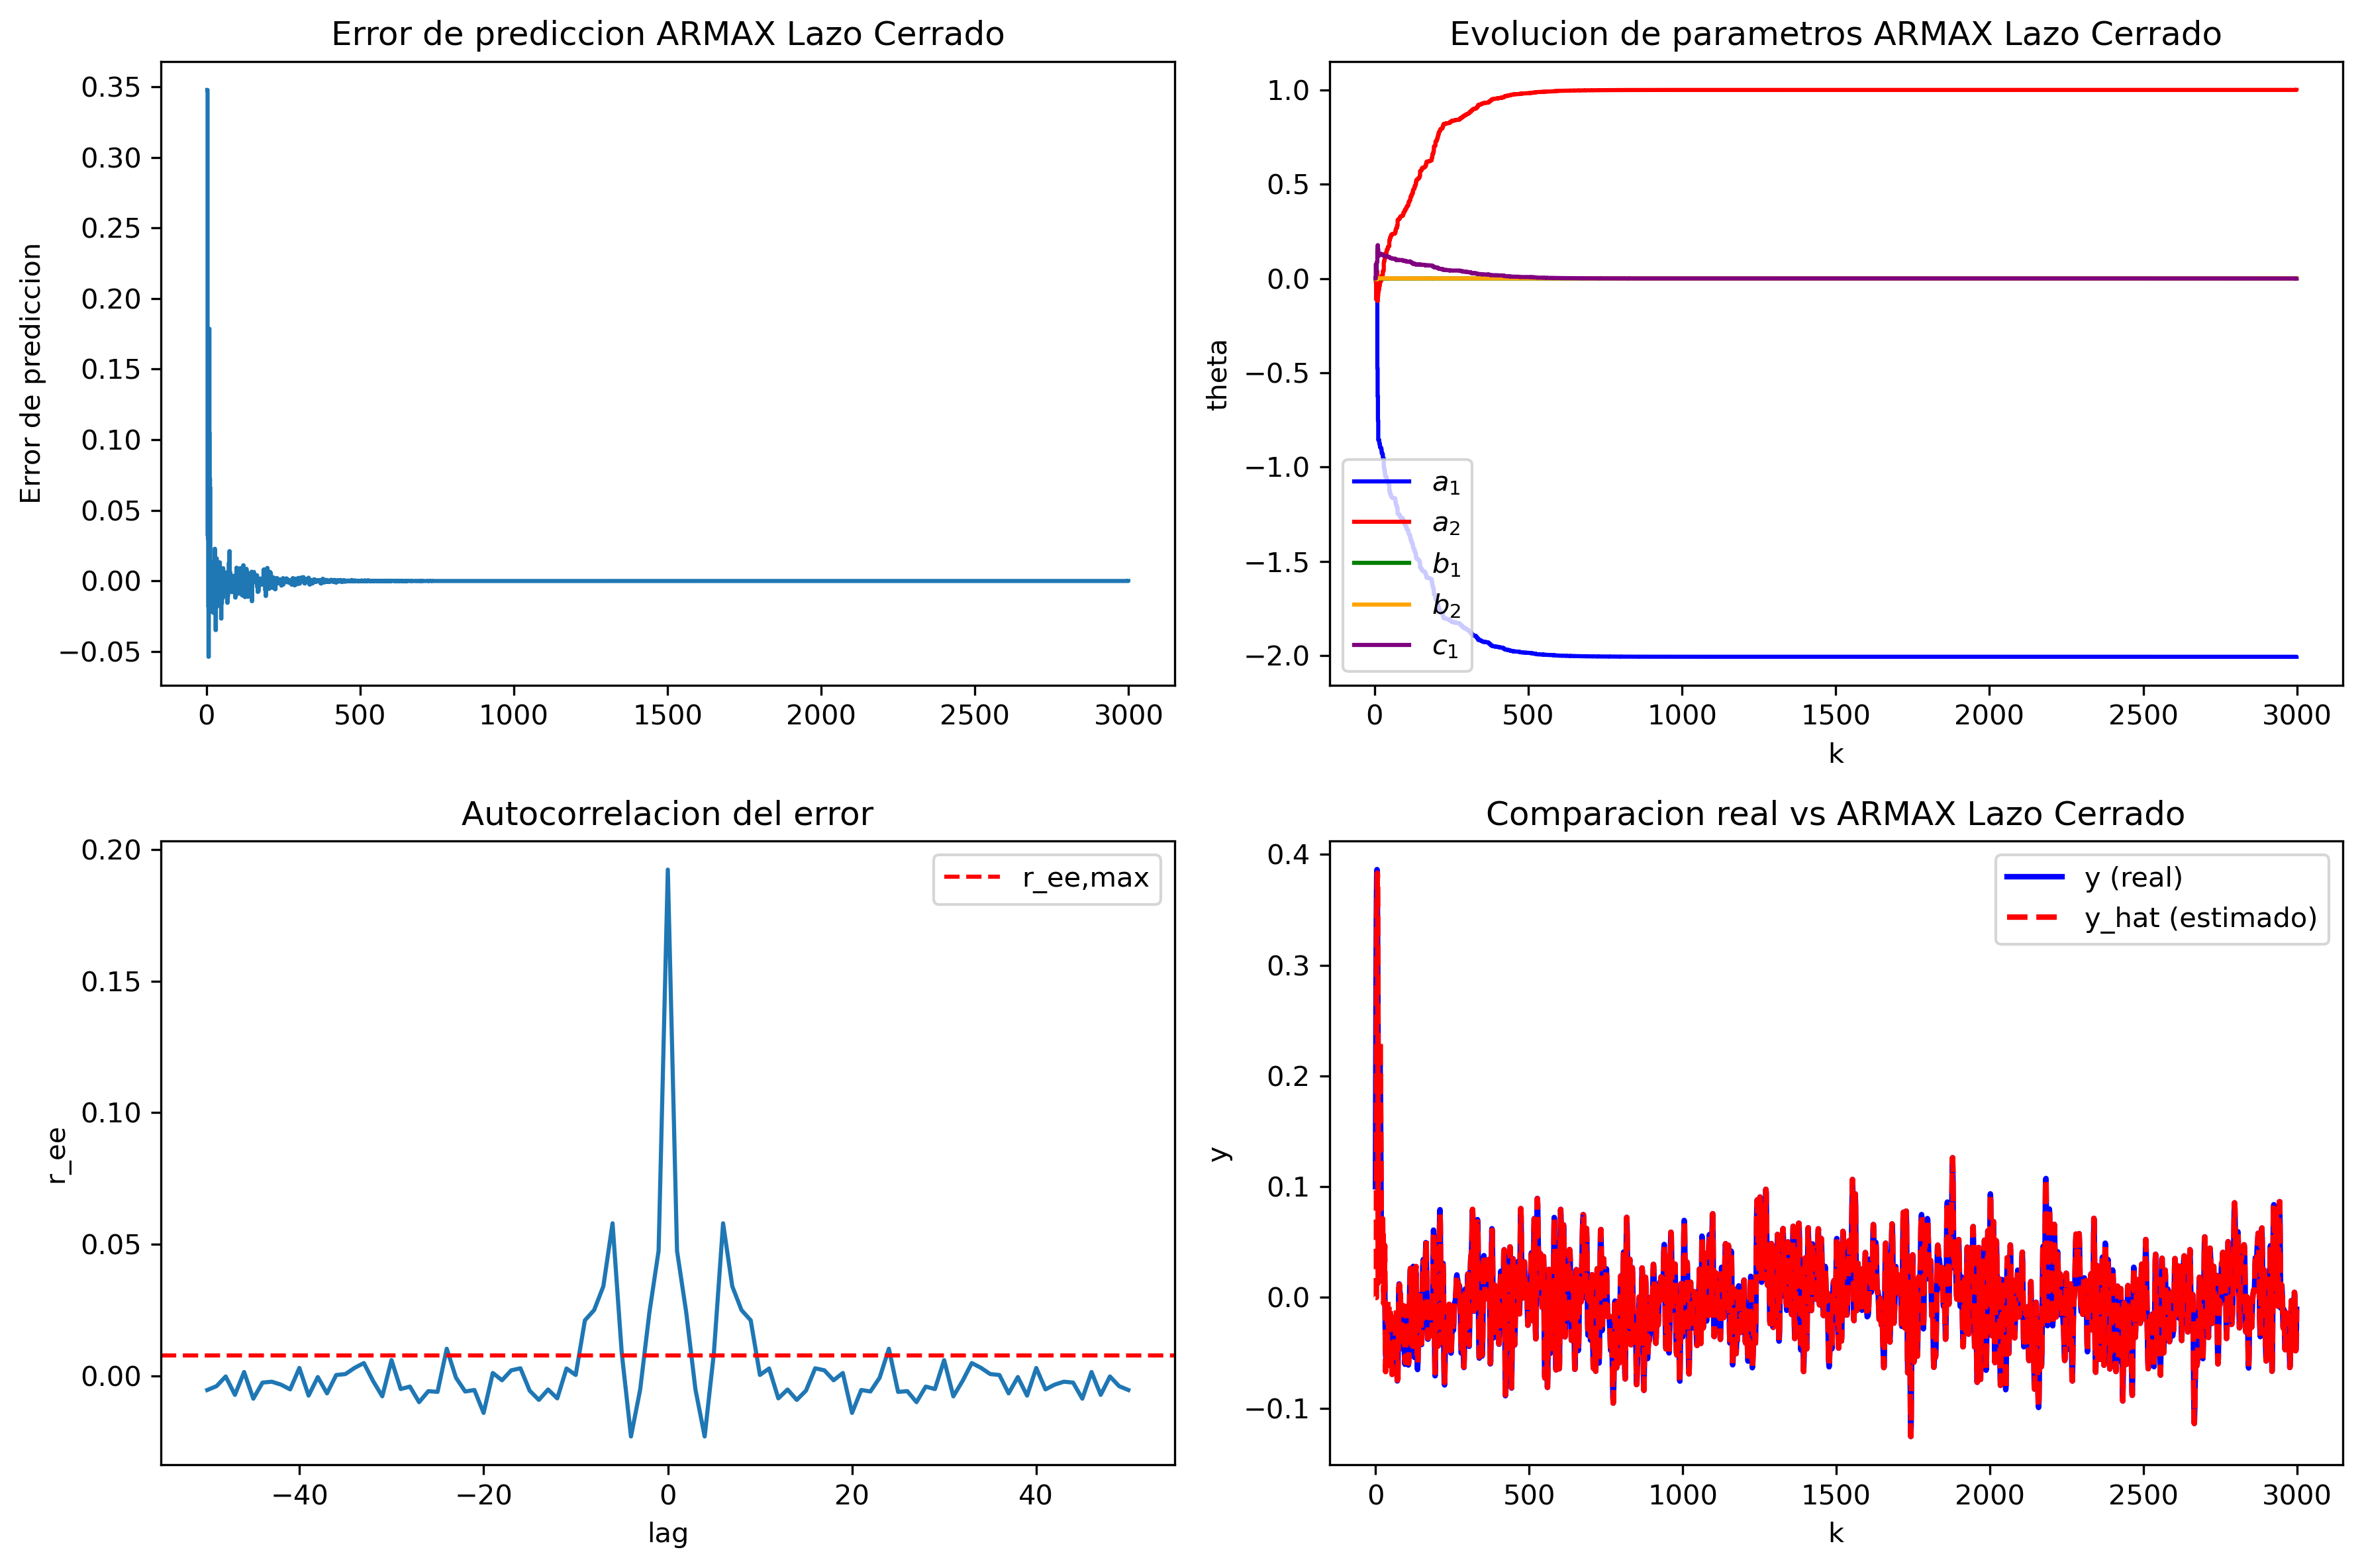
\includegraphics[width=0.9\textwidth]{imagenes_identificacion_pi_control/armax_closed_loop_identification.png}
\end{center}
\end{frame}

\begin{frame}{Validación del Modelo Identificado}
\begin{center}
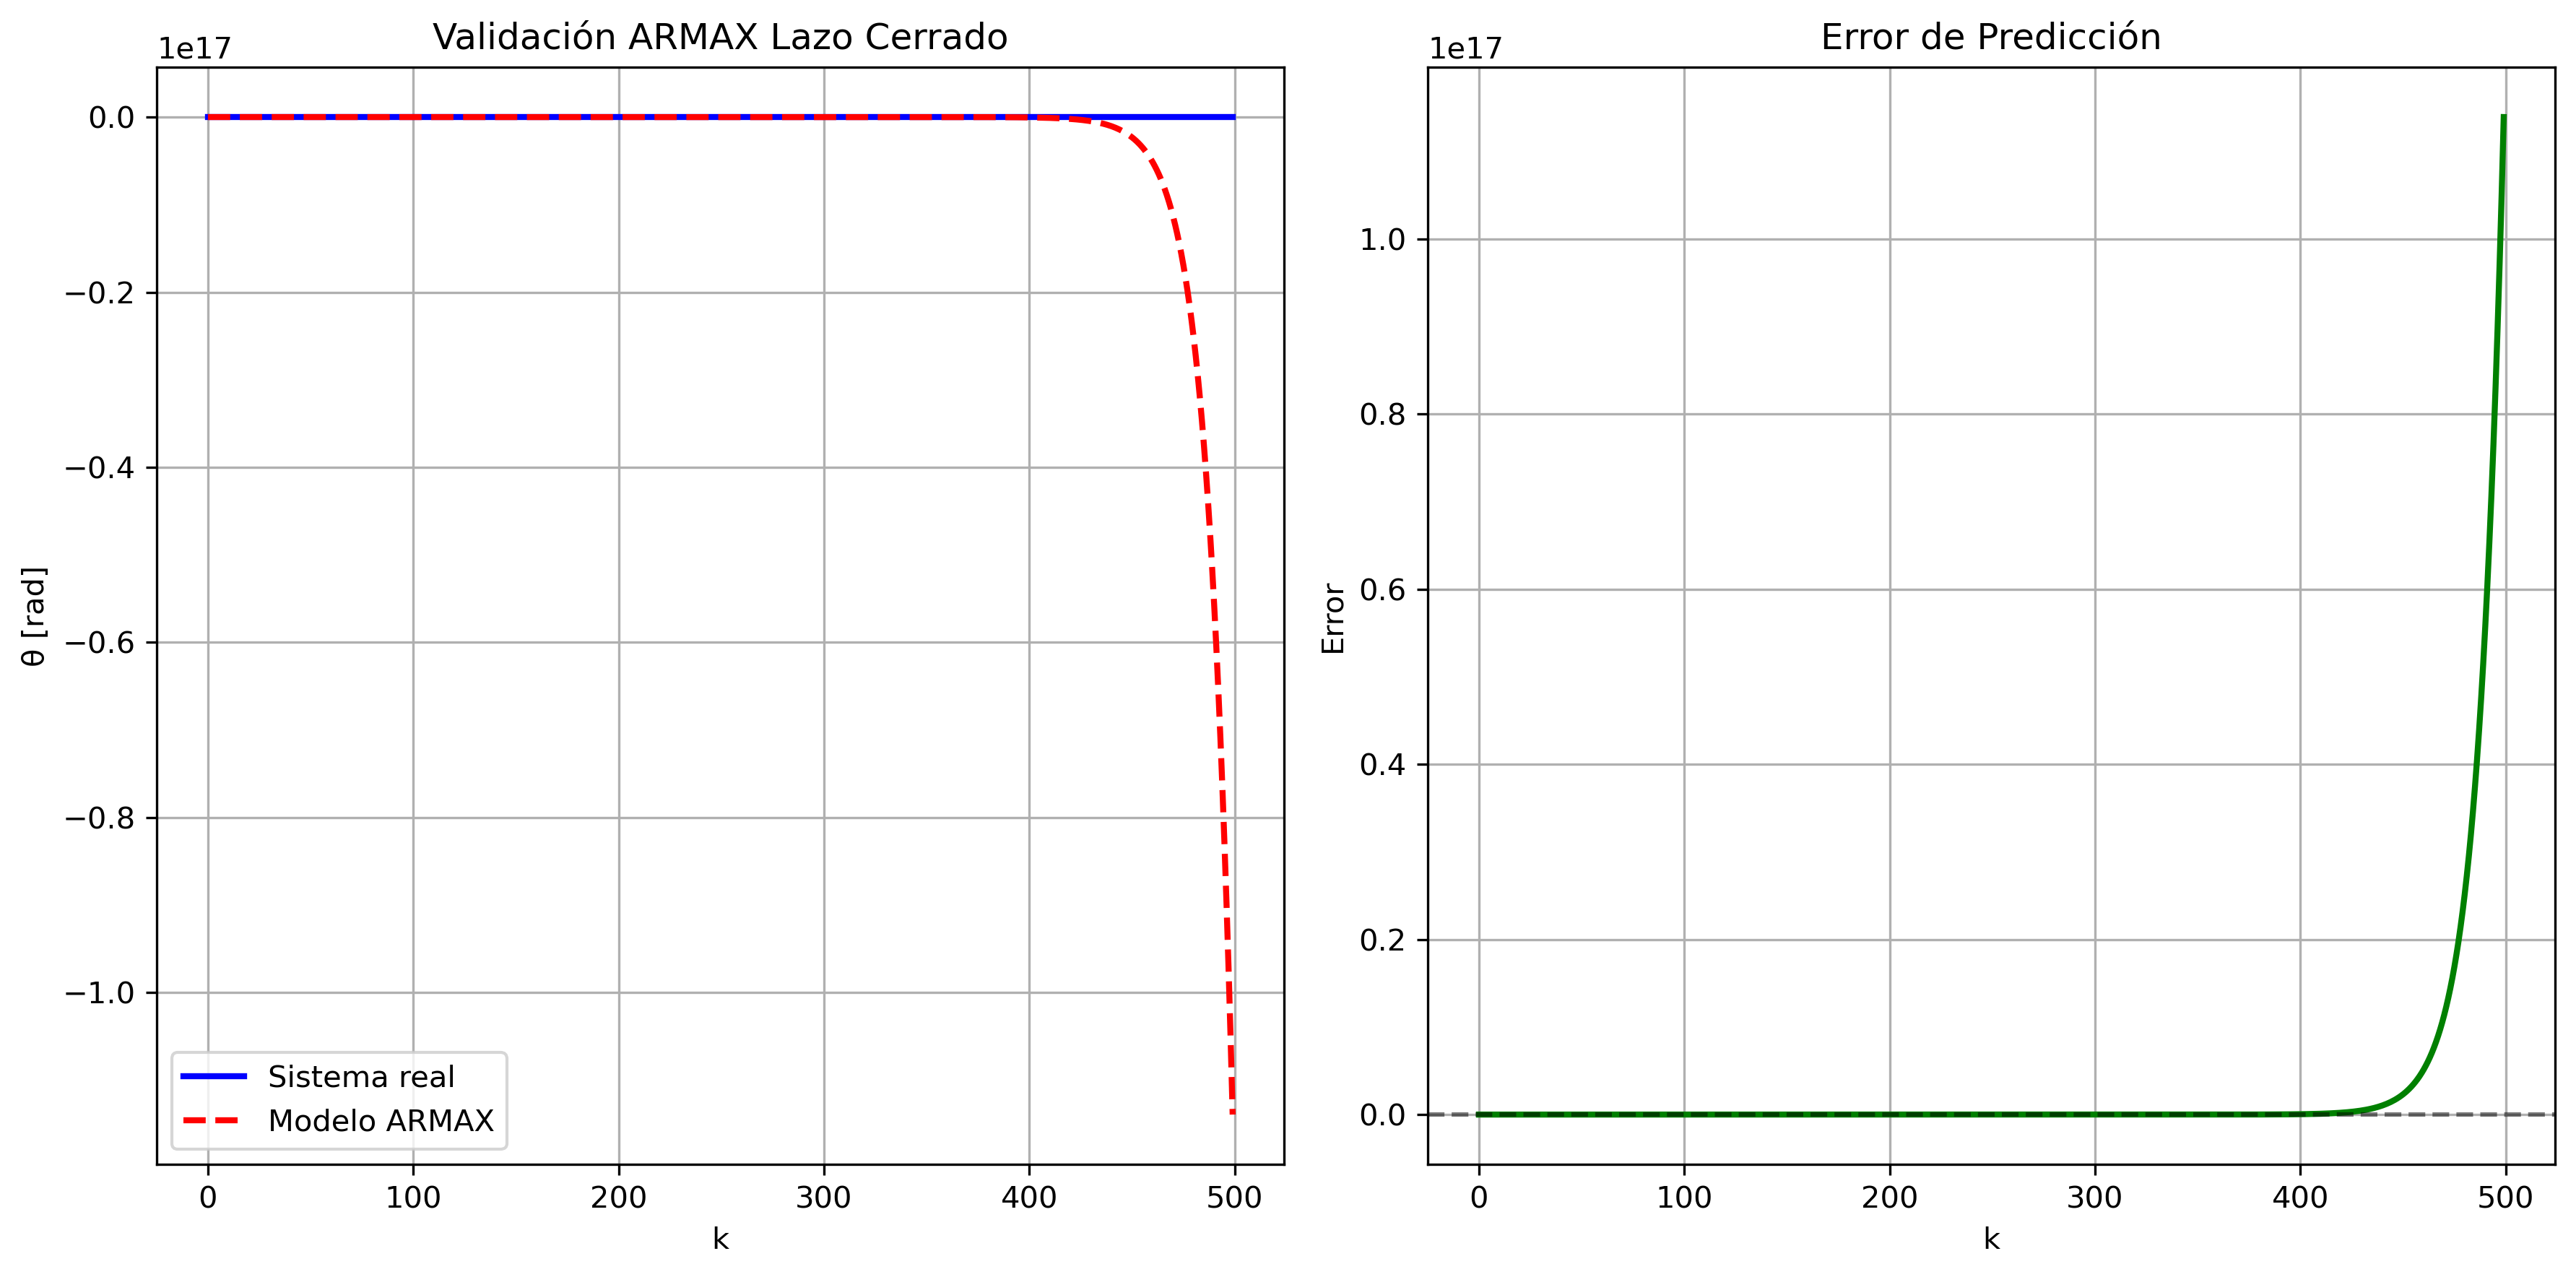
\includegraphics[width=0.8\textwidth]{imagenes_identificacion_pi_control/armax_closed_loop_validation.png}
\end{center}
\begin{itemize}
\item Comparación temporal: sistema real vs. modelo identificado
\item Error de predicción: $RMSE = 1.70 \times 10^{33}$
\item MSE validación: $2.90 \times 10^{66}$
\end{itemize}
\end{frame}

\begin{frame}{Conclusión: Control + Identificación en Lazo Cerrado}
\begin{block}{Resultados del Enfoque Híbrido}
\begin{itemize}
\item Control PID: estabilización del péndulo inestable
\item Identificación ARMAX: parámetros identificados en sistema controlado
\item Sistema resultante: estable con dinámica modificada
\end{itemize}
\end{block}

\begin{block}{Características del Enfoque}
\begin{itemize}
\item Control previo requerido para sistemas inestables
\item Identificación posterior en lazo cerrado
\item Parámetros representan dinámica global controlada
\item Alternativa a identificación directa de sistemas abiertos
\end{itemize}
\end{block}
\end{frame}

\end{document}
